%%%%%%%%%%%%%%%%%%%%%%%%%%%%%%%%%%%%%%%%%
% Masters/Doctoral Thesis 
% LaTeX Template
% Version 2.5 (27/8/17)
%
% This template was downloaded from:
% http://www.LaTeXTemplates.com
%
% Version 2.x major modifications by:
% Vel (vel@latextemplates.com)
%
% This template is based on a template by:
% Steve Gunn (http://users.ecs.soton.ac.uk/srg/softwaretools/document/templates/)
% Sunil Patel (http://www.sunilpatel.co.uk/thesis-template/)
%
% Template license:
% CC BY-NC-SA 3.0 (http://creativecommons.org/licenses/by-nc-sa/3.0/)
%
%%%%%%%%%%%%%%%%%%%%%%%%%%%%%%%%%%%%%%%%%

%----------------------------------------------------------------------------------------
%   PACKAGES AND OTHER DOCUMENT CONFIGURATIONS
%----------------------------------------------------------------------------------------

\PassOptionsToPackage{spanish,mexico}{babel}

\documentclass[
11pt, % The default document font size, options: 10pt, 11pt, 12pt
%oneside, % Two side (alternating margins) for binding by default, uncomment to switch to one side
spanish, % ngerman for German
singlespacing, % Single line spacing, alternatives: onehalfspacing or doublespacing
%draft, % Uncomment to enable draft mode (no pictures, no links, overfull hboxes indicated)
%nolistspacing, % If the document is onehalfspacing or doublespacing, uncomment this to set spacing in lists to single
%liststotoc, % Uncomment to add the list of figures/tables/etc to the table of contents
%toctotoc, % Uncomment to add the main table of contents to the table of contents
%parskip, % Uncomment to add space between paragraphs
%nohyperref, % Uncomment to not load the hyperref package
headsepline, % Uncomment to get a line under the header
%chapterinoneline, % Uncomment to place the chapter title next to the number on one line
%consistentlayout, % Uncomment to change the layout of the declaration, abstract and acknowledgements pages to match the default layout
]{MastersDoctoralThesis} % The class file specifying the document structure

\usepackage[utf8]{inputenc} % Required for inputting international characters
\usepackage[T1]{fontenc} % Output font encoding for international characters

\usepackage{mathpazo} % Use the Palatino font by default

\usepackage[backend=bibtex,style=ieee,natbib=true]{biblatex} % Use the bibtex
% backend with the authoryear citation style (which resembles APA)

\addbibresource{bibliografia.bib} % The filename of the bibliography

\usepackage[autostyle=true]{csquotes} % Required to generate language-dependent quotes in the bibliography

\usepackage[spanish]{babel}
\selectlanguage{spanish} 

\usepackage{subcaption}

\usepackage[inline]{enumitem}

\usepackage{titlesec}

\usepackage[linesnumbered,lined,ruled,vlined,spanish,onelanguage]{algorithm2e}

\usepackage{mathtools}
\newcommand\Set[2]{\{\,#1\mid#2\,\}}
\newcommand\SET[2]{\Set{#1}{\text{#2}}}

\usepackage{siunitx}

\usepackage{url}

\usepackage{hyperref}

\usepackage{listings}

\usepackage{color}

\usepackage{dirtree}

\definecolor{gray}{rgb}{0.4,0.4,0.4}
\definecolor{darkblue}{rgb}{0.0,0.0,0.6}
\definecolor{cyan}{rgb}{0.0,0.6,0.6}

\lstset{
  basicstyle=\ttfamily,
  columns=fullflexible,
  showstringspaces=false,
  commentstyle=\color{gray}\upshape
}

\lstdefinelanguage{XML}
{
  morestring=[b]",
  morestring=[s]{>}{<},
  morecomment=[s]{<?}{?>},
  stringstyle=\color{black},
  identifierstyle=\color{darkblue},
  keywordstyle=\color{cyan},
  morekeywords={xmlns,version,type}% list your attributes here
}

%----------------------------------------------------------------------------------------
%   MARGIN SETTINGS
%----------------------------------------------------------------------------------------

\geometry{
    paper=letterpaper, % Change to letterpaper for US letter
    inner=2.5cm, % Inner margin
    outer=3.8cm, % Outer margin
    bindingoffset=.5cm, % Binding offset
    top=1.5cm, % Top margin
    bottom=1.5cm, % Bottom margin
    %showframe, % Uncomment to show how the type block is set on the page
}

%----------------------------------------------------------------------------------------
%   THESIS INFORMATION
%----------------------------------------------------------------------------------------

\thesistitle{Protocolo de enrutamiento para VANETs con nodos autoconfigurables} % Your thesis title, this is used in the title and abstract, print it elsewhere with \ttitle
\supervisor{Jesús Alfredo Martínez Nuño} % Your supervisor's name, this is used in the title page, print it elsewhere with \supname
\examiner{} % Your examiner's name, this is not currently used anywhere in the template, print it elsewhere with \examname
\degree{Maestro en Ciencias en Sistemas Computacionales Móviles} % Your degree name, this is used in the title page and abstract, print it elsewhere with \degreename
\author{Adrián Juárez Monroy} % Your name, this is used in the title page and abstract, print it elsewhere with \authorname
\addresses{} % Your address, this is not currently used anywhere in the template, print it elsewhere with \addressname

\subject{Biological Sciences} % Your subject area, this is not currently used anywhere in the template, print it elsewhere with \subjectname
\keywords{} % Keywords for your thesis, this is not currently used anywhere in the template, print it elsewhere with \keywordnames
\university{\href{http://www.ipn.mx}{Instituto Politécnico Nacional}} % Your university's name and URL, this is used in the title page and abstract, print it elsewhere with \univname
\department{\href{http://escom.ipn.mx/posgrado/}{Sección de Estudios de Posgrado e Investigación}} % Your department's name and URL, this is used in the title page and abstract, print it elsewhere with \deptname
\group{Comunicaciones para el cómputo móvil} % Your research group's name and URL, this is used in the title page, print it elsewhere with \groupname
\faculty{\href{http://www.escom.ipn.mx/}{Escuela Superior de Cómputo}} % Your faculty's name and URL, this is used in the title page and abstract, print it elsewhere with \facname

\AtBeginDocument{
\hypersetup{pdftitle=\ttitle} % Set the PDF's title to your title
\hypersetup{pdfauthor=\authorname} % Set the PDF's author to your name
\hypersetup{pdfkeywords=\keywordnames} % Set the PDF's keywords to your keywords
}

\begin{document}

\frontmatter % Use roman page numbering style (i, ii, iii, iv...) for the pre-content pages

\pagestyle{plain} % Default to the plain heading style until the thesis style is called for the body content

%----------------------------------------------------------------------------------------
%   TITLE PAGE
%----------------------------------------------------------------------------------------

\begin{titlepage}
    \thispagestyle{empty}
    \setlength{\headheight}{0pt}
    \begin{minipage}[c][0.17\textheight][c]{0.22\textwidth}
        \begin{center}
            
\includegraphics[width=2.7cm]{Figuras/logo-ipn.png}
        \end{center}
    \end{minipage}
    \begin{minipage}[c][0.195\textheight][t]{0.73\textwidth}
        \begin{center}
            \vspace{0.3cm}
            \textsc{\Large \univname}
            \vspace{0.8cm}
            \hrule height 2.5pt
            \vspace{0.2cm}
            \hrule height 1pt
            \vspace{0.8cm}
            \textsc{\facname\\
            \deptname}
        \end{center}
    \end{minipage}

    \begin{minipage}[c][0.81\textheight][t]{0.22\textwidth}
        \vspace*{5mm}
        \begin{center}
            \hskip2.0mm
            \vrule width 1pt height 13cm
            \vspace{5mm}
            \hskip2pt
            \vrule width 2.5pt height 13cm
            \hskip2mm
            \vrule width 1pt height 13cm \\
            \vspace{3mm}
            
\includegraphics[height=2.3cm]{Figuras/logo-escom.png}
        \end{center}
    \end{minipage}
    \begin{minipage}[c][0.81\textheight][t]{0.73\textwidth}
        \begin{center}
            \vspace{1cm}

                \textsc{\large \ttitle}\\

            \vspace{2.5cm}

            \textsc{\Large Tesis}\\
            \vspace{0.5cm}

            \textsc{\large que para obtener el grado de}\\
            \vspace{0.5cm}

            \textsc{\large \degreename}\\
            \vspace{0.5cm}

            \textsc{\large presenta}\\
            \vspace{0.5cm}

            \textsc{\large \authorname}\\
            \vspace{2.5cm}

            \textsc{\large Directores:}\\
            \vspace{0.5cm}

            \textsc{\large Dr. Manuel Salazar Ramírez \\
M. en C. Jesús Alfredo Martínez Nuño}\\
            \vspace{0.5cm}

            \large{Ciudad de México, \today}
        \end{center}
    \end{minipage}
\end{titlepage}

%----------------------------------------------------------------------------------------
%   QUOTATION PAGE
%----------------------------------------------------------------------------------------

\vspace*{0.2\textheight}

\noindent\enquote{\itshape Cita.}\bigbreak

\hfill Autor

%----------------------------------------------------------------------------------------
%   ABSTRACT PAGE
%----------------------------------------------------------------------------------------

\begin{abstract}
\addchaptertocentry{\abstractname} % Add the abstract to the table of contents
Resumen
\end{abstract}

%----------------------------------------------------------------------------------------
%   ACKNOWLEDGEMENTS
%----------------------------------------------------------------------------------------

\begin{acknowledgements}
\addchaptertocentry{\acknowledgementname} % Add the acknowledgements to the table of contents
Agradecimientos\ldots
\end{acknowledgements}

%----------------------------------------------------------------------------------------
%   LIST OF CONTENTS/FIGURES/TABLES PAGES
%----------------------------------------------------------------------------------------

\tableofcontents % Prints the main table of contents

\listoffigures % Prints the list of figures

\listoftables % Prints the list of tables

%----------------------------------------------------------------------------------------
%   ABBREVIATIONS
%----------------------------------------------------------------------------------------

% \begin{abbreviations}{ll} % Include a list of abbreviations (a table of two columns)
% 
% % AAP
% \textbf{AAP} & \textit{\textbf{A}ddress \textbf{A}uto-configuration \textbf{P}rotocol}\\
% & Protocolo de autoconfiguración de direcciones\\
% 
% % AS
% \textbf{AS} & \textit{\textbf{A}utonomous \textbf{S}ystem}\\
% & Sistema autónomo\\
% 
% % DAD
% \textbf{DAD} & \textit{\textbf{D}uplicate \textbf{A}ddress \textbf{D}etection}\\
% & Detección de direcciones duplicadas\\
% 
% % EGP
% \textbf{EGP} & \textit{\textbf{E}xterior \textbf{G}ateway \textbf{P}rotocol}\\
% & Protocolo de puerta de enlace exterior\\
% 
% % GPSR
% \textbf{GPSR} & \textit{\textbf{G}reedy \textbf{P}erimeter \textbf{S}tateless \textbf{R}outing}\\
% & Enrutamiento voraz y de perímetro sin estado\\
% 
% % HTTP
% \textbf{HTTP} & \textit{\textbf{H}yper\textbf{T}ext \textbf{T}ransfer \textbf{P}rotocol}\\
% & Enrutamiento voraz y de perímetro sin estado\\
% 
% % IGP
% \textbf{IGP} & \textit{\textbf{I}nterior \textbf{G}ateway \textbf{P}rotocol}\\
% & Protocolo de puerta de enlace interior\\
% 
% % MANET
% \textbf{MANET} & \textit{\textbf{M}obile \textbf{A}d hoc \textbf{N}etwork}\\
% & Red \textit{ad hoc} móvil\\
% 
% % ND
% \textbf{ND} & \textit{\textbf{N}eighbor \textbf{D}iscovery}\\
% & Descubrimiento de vecinos\\
% 
% % vanet
% \textbf{VANET} & \textit{\textbf{V}ehicular \textbf{A}d hoc \textbf{N}etwork}\\ 
% & Red \textit{ad hoc} vehicular\\
% 
% \end{abbreviations}

%----------------------------------------------------------------------------------------
%   DEDICATION
%----------------------------------------------------------------------------------------

\dedicatory{Dedicatoria\ldots} 

%----------------------------------------------------------------------------------------
%   THESIS CONTENT - CHAPTERS
%----------------------------------------------------------------------------------------

\mainmatter % Begin numeric (1,2,3...) page numbering

\pagestyle{thesis} % Return the page headers back to the "thesis" style

% Include the chapters of the thesis as separate files from the Chapters folder
% Uncomment the lines as you write the chapters

%----------------------------------------------------------------------------------------

% Define some commands to keep the formatting separated from the content 
\newcommand{\keyword}[1]{\textbf{#1}}
\newcommand{\tabhead}[1]{\textbf{#1}}
\newcommand{\code}[1]{\texttt{#1}}
\newcommand{\file}[1]{\texttt{\bfseries#1}}
\newcommand{\option}[1]{\texttt{\itshape#1}}
\setlength{\parskip}{0.5em}

%----------------------------------------------------------------------------------------

\chapter{Introducción}
%-----------------------------------
%   INTRODUCCIÓN
%-----------------------------------
\label{ch:introduccion}

La evolución de los sistemas de comunicación se ha acelerado importantemente en
las últimas décadas. El primer gran paso en el desarrollo de estos sistemas fue
el uso de ondas de radiofrecuencia para enviar mensajes entre un transmisor y
un receptor. Después, se crearon protocolos y dispositivos más complejos para
formar redes que permitieron el intercambio de información entre más de dos
computadoras. Esto dio origen a la Internet, que hace posible que millones de
dispositivos puedan compartir información desde casi cualquier parte del mundo.

Con el desarrollo de los dispositivos móviles, como los teléfonos inteligentes,
las redes celulares se han convertido en uno de los sistemas de comunicación
más usados en el mundo. Estas redes permiten tener conectividad incluso estando
en movimiento. Sin embargo, la conexión está restringida al área de cobertura de
las antenas. Existen lugares donde no se cuenta con infraestructura de red, por
lo que no hay posibilidad de comunicarse aunque se cuente con un dispositivo
móvil. Debido a estas limitaciones, es natural considerar a las redes móviles
sin infreastructura fija como el siguiente paso en la evolución de los sistemas
de telecomunicaciones.

Las redes móviles \textit{ad hoc}, o MANETs (\textit{mobile ad hoc networks}),
se forman únicamente por dispositivos móviles. Estas redes no cuentan con
infraestructura fija, por lo que los dispositivos deben configurse de manera
autónoma para comunicarse entre sí y formar una red. No obstante, las
características de estas redes implican nuevos retos que se tienen que superar
para proporcionar un servicio confiable. Su principal característica es que no
tienen una topología fija, ya que los nodos tienen la libertad de moverse sin
restricciones. Esto hace que el enrutamiento sea el problema más difícil de
resolver \cite{Li2008}.

Un tipo de MANET que ha despertado gran interés en los últimos años, son las
redes \textit{ad hoc} vehiculares, o VANETs (\textit{vehicular ad hoc
networks}). Cada vehículo cuenta con un dispositivo que le permite comunicarse
con los demás para formar la red. Debido a que los vehículos se mueven a altas
velocidades y cada uno sigue una ruta distinta, los enlaces tienen duraciones
muy cortas. Es por esto que la topología cambia con más frecuencia y el
enrutamiento se vuelve aún más complicado \cite{Meneguette2018}.

Existen muchos tipos de aplicaciones para las VANETs, que se pueden clasificar
en dos principales grupos. Las aplicaciones de seguridad tienen como objetivo
proporcionar a los conductores información útil para prevenir accidentes. Las
aplicaciones de no-seguridad se enfocan en servicios como compartir y descargar
archivos, monitorización del tráfico, mensajería, entre otros
\cite{Meneguette2018}.

El objetivo de este trabajo es diseñar un sistema de comunicación basado en una
VANET que permita a las personas compartir información. Esto sería
particularmente útil en lugares o situaciones en las que no haya disponible una
red de infraestructura fija que permitan a las personas mantenerse comunicarse.
Para esto, se propone un protocolo de enrutamiento para VANETs que cuente con
un mecanismo que le proporcione a cada dispositivo la capacidad de configurarse
autónomamente.

\section{Formulación del problema}
%-----------------------------------
%   FORMULACIÓN DEL PROBLEMA
%-----------------------------------
\label{sec:formulacion_del_problema}

Para que la red pueda proporcionar un buen servicio, se necesita que la mayor
cantidad de paquetes lleguen a su destino en el menor tiempo posible. Los
protocolos de enrutamiento son los principales responsables de que se cumplan
estas condiciones. En las redes cableadas, la topología sufre cambios muy rara
vez, por lo que se pueden determinar las rutas conociendo la topología.
Pero en las MANETs ocurre exactamente lo opuesto, por lo que el enrutamiento es
considerablemente más complicado.

En las MANETs, los enlaces inalámbricos entre los dispositivos pueden tener
duraciones muy cortas como consecuencia del constante movimiento de los
dispositivos. Por esta razón, una vez que se encuentra una ruta hacia algún otro
dispositivo en la red, toda la ruta quedaría inutilizable tan sólo con
desaparecer uno de los enlaces que la forman. Este problema se acentúa aún más
en las VANETs, ya que los vehículos se mueven a velocidades aún más altas.

Se han desarrollado diferentes enfoques para resolver el problema del
enrutamiento en este tipo de redes. Uno en particular que ha mostrado buenos
resultados implica considerar la ubicación de los dispositivos en lugar de la
topología a la hora de buscar una ruta. El remitente indica en cada paquete la
dirección y la ubicación del destinatario, lo que es de mucha ayuda para
determinar hacia dónde se debe transmitir. Además de esto, apoyarse de mapas ha
servido para mejorar la calidad del enrutamiento \cite{Lochert2003}. Sin
embargo, se presenta otro problema: cómo saber la ubicación del destinatario
\cite{Brendha2017}.

Por otro lado, antes de poder comenzar a hacer el enrutamiento, es
indispensable que cada nodo de la red tenga una dirección, ya que es la manera
en la que se identifica ante los demás. Las direcciones permiten saber qué nodo
envía un paquete y a qué nodo va destinado. En las redes de infraestructura
fija, la asignación de direcciones se hace de manera centralizada, generalmente
mediante un servidor DHCP (\textit{Dynamic Host Configuration
Protocol})\footnote{Protocolo de configuración dinámica de \textit{hosts}.}.
Hacerlo de este modo garantiza que ninguna dirección esté asignada a dos nodos
al mismo tiempo. Sin embargo, en una VANET no es tan simple lograr que un solo
nodo administre las direcciones de todos los demás \cite{Korichi2018}.

Dicho lo anterior, para poder desplegar una VANET que proporcione un servicio de
comunicación, lo primero que se necesita es un mecanismo descentralizado que
permita que los dispositivos obtener una dirección única. Una vez que los
dispositivos cuenten con una dirección, antes de enviar un paquete, se necesita
un método que les permita obtener la ubicación del destinatario. Una vez que
tienen la ubicación del destinatario, se necesita que un protocolo de
enrutamiento haga llegar los paquetes al dispositivo correspondiente mediante
saltos entre dispositivos intermedios.

\section{Preguntas de investigación}
%-----------------------------------
%   PREGUNTAS DE INVESTIGACIÓN
%-----------------------------------
\label{sec:preguntas_de_investigacion}

\begin{itemize}
  \item ¿Cómo se puede realizar la configuración de direcciones de los nodos en
  una VANET?
  \item ¿Cómo se pueden determinar las rutas en una VANET con ayuda de un mapa?
\end{itemize}

\section{Objetivos}
%-----------------------------------
%   OBJETIVOS
%-----------------------------------
\label{subsec:objetivos}

\subsection{Objetivo general}
%-----------------------------------
%   OBJETIVO GENERAL
%-----------------------------------
\label{subsec:objetivo_general}

Diseñar un protocolo de enrutamiento para VANETs que permita usar la información
de las vialidades para determinar las rutas y que permita a cada vehículo
configurar su propia dirección única.

\subsection{Objetivos específicos}
%-----------------------------------
%   OBJETIVOS ESPECÍFICOS
%-----------------------------------
\label{subsec:objetivos_especificos}

\begin{itemize}
  \item Diseñar el protocolo de autoconfiguración de direcciones.
  \item Diseñar el protocolo de enrutamiento.
  \item Evaluar el desepeño del protocolo mediante simulaciones.
\end{itemize}

\section{Justificación}
%-----------------------------------
%   JUSTIFICACIÓN
%-----------------------------------
\label{sec:justificacion}

Debido a las características de las VANETs, la diversidad de aplicaciones que
tienen y los diferentes escenarios en los que se pueden aplicar, el enrutamiento
es un enorme reto que no se ha logrado superar por completo. No existen
protocolos de enrutamuiento bien consolidados para estas redes, como sí los hay
para las redes de infraestructura fija. Por esta razón, este es un tema de
investigación muy activo actualmente.

La mayoría de estos protocolos se enfocan en aplicaciones como seguridad vial,
monitorización del tráfico, entretenimiento, entre otras. El protocolo
propuesto en este trabajo se enfoca en una aplicación diferente, que es
proporcionar un servicio de comunicación alternativo en caso de no tener acceso
a redes de infraestructura fija.

Existe una gran cantidad de protocolos para VANETs que se han propuesto en los
últimos años. Con el desarrollo de nuevos protocolos, eventualmente se
logrará ratificar estándares para diferentes aplicaciones o condiciones.

%-----------------------------------
%   VANETS
%-----------------------------------
\chapter{Redes \textit{ad hoc} vehiculares (VANETs)}

\label{ch:vanets}

% En general, toda red sirve para compartir información entre dispositivos, y
% todas comparten la misma arquitectura. No obstante, la principal diferencia
% entre los distintos tipos de redes se encuentra en los protocolos de
% comunicación. Los protocolos para redes móviles son más complejos que los
% protocolos para redes de infraestructura fija. Esto es porque la comunicación
% inalámbrica tiene problemas inherentes que no se presentan en la comunicación
% alámbrica. Los protocolos de comunicación son los que se encargan de lidiar con
% estos problemas.
% 
% En este capítulo, se presenta una introducción a las VANETs, para entender qué
% dificultades presentan para el desarrollo de los protocolos de comunicación.
% También se describe el protocolo IPv6, que es el que determina la estuctura de
% los paquetes de información que circulan a través de una red, además de las
% direcciones que identifican a cada nodo. Después, se describe el problema de la
% autoconfiguración de nodos en las redes móviles, y algunos protocolos que se han
% propuesto para resolverlo. Finalmente, se presentan los diferentes enfoques de
% enrutamiento y ejemplos de protocolos de enrutamiento para redes \textit{ad
% hoc}.

Una red es un conjunto de dispositivos que están interconectados mediante
enlaces que les permiten intercambiar mensajes. Estos dispositivos, denominados
\textit{nodos} a partir de aquí, pueden ser computadoras, teléfonos,
enrutadores, o cualquier tipo de dispositivo que sea capaz de comunicarse con
los demás \cite{Marsic2013}.

La \textit{topología} de una red el conjunto de nodos que la forman y los
enlaces entre ellos \cite{Dordal2014}. La topología, por lo general, se
representa con un grafo, en el que los vértices son los dispositivos que forman
la red, y las aristas son las conexiones físicas entre ellos. En la figura
\ref{fig:topologias} se muestran dos topologías diferentes.

\begin{figure}[th]
\centering

\begin{subfigure}[b]{0.45\textwidth}
\centering
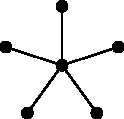
\includegraphics{topologia_estrella}
\caption[Topología de estrella.]{Topología de estrella.}
\label{fig:topologia_estrella}
\end{subfigure}
\hfill
\begin{subfigure}[b]{0.45\textwidth}
\centering
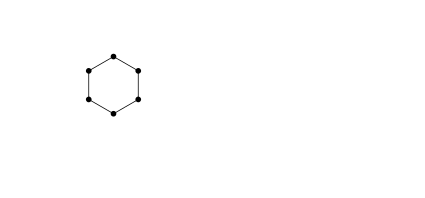
\includegraphics{topologia_anillo}
\caption[Topología de anillo]{Topología de anillo.}
\label{fig:topologia_anillo}
\end{subfigure}
\hfill
\begin{subfigure}[b]{0.45\textwidth}
\centering
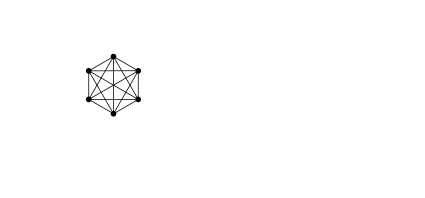
\includegraphics{topologia_malla}
\caption[Topología de malla]{Topología de malla.}
\label{fig:topologia_malla}
\end{subfigure}

\decoRule
\caption[Dos topologías diferentes]{Dos topologías diferentes.}
\label{fig:topologias}
\end{figure}

Una VANET es una red inalámbrica donde los nodos son dispositivos a bordo de
vehículos. En este documento, cuando se esté hablando de una VANET, entiéndase
``nodo'' y ``vehículo'' como sinónimos. Al tratarse de una red que no depende de
infraestructura fija, los nodos funcionan como enrutadores y \textit{hosts} al
mismo tiempo. La figura \ref{fig:vanet} muestra la representación de una VANET.

\begin{figure}[th]
\centering
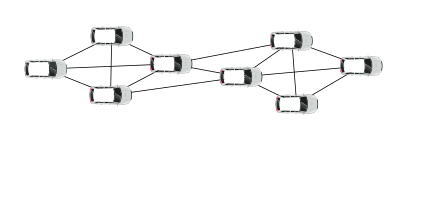
\includegraphics{vanet}
\decoRule
\caption[Red \textit{ad hoc} vehicular]{Red \textit{ad hoc} vehicular.}
\label{fig:vanet}
\end{figure}

%-----------------------------------
%   CARACTERÍSTICAS DE UNA VANET
%-----------------------------------
\section{Características de una VANET}

\label{sec:caracteristicas_de_una_vanet}

A continuación, se presentan las características que distinguen a las VANETs de
otros tipos de redes inalámbricas \cite{Meneguette2018}:

\keyword{Autoorganización} -- Al ser una red descentralizada, necesita
mecanismos que permitan a los nodos autoconfigurarse.

\keyword{Movilidad} -- Los nodos de una VANET se mueven muy rápidamente. Sin
embargo, la movilidad está restringida por la infraestructura vial, lo que hace
que sea relativamente predecible.

\keyword{Velocidad de transmisión} -- La velocidad de transmisión debe ser
rápida, debido a que dos vehículos pueden quedar fuera de alcance en pocos
segundos.

\keyword{Topología} -- Aunque la posición de los vehículos está sujeta a las
restricciones de las calles, la alta movilidad provoca cambios frecuentes en
la topología.

\keyword{Energía} -- En la mayoría de las redes inalámbricas, los nodos son
teléfonos móviles, computadoras portátiles, tabletas, u otros dispositivos que
dependen de una fuente de energía limitada. En una VANET, los nodos disponen de
una fuente de energía más abundante, por lo que también pueden contar con mayor
poder de cómputo.

\keyword{Ancho de banda} -- Los nodos pueden contar con más de un dispositivo de
comunicación, haciendo posible conectarse a diferentes redes  para lidiar con la
pérdida de conectividad y aumentar el ancho de banda.

\keyword{Fragmentación de la red} -- En ocasiones, un subconjunto de los nodos
pueden quedar aislados, debido a que su radio de comunicación no es suficiente
para alcanzar al resto de los nodos.

Las VANETs abren un gran abanico de aplicaciones para proporcionar diferentes
servicios a conductores y pasajeros. Algunas de las aplicaciones son las
siguientes \cite{Meneguette2018}:

\keyword{Aplicaciones de seguridad} -- Tienen como principal objetivo la
reducción del número de accidentes viales. Por ejemplo, advertencia cooperativa
de colisiones, asistencia para el cambio de carril, control de peligros en la
carretera, vigilancia del tráfico, notificación posterior a un accidente, etc.

\keyword{Aplicaciones de no-seguridad} -- Están destinadas a ofrecer comodidad
durante el viaje. Algunos ejemplos son notificación de servicios y páginas
amarillas, monitorización de vehículos, juegos, intercambio de información,
etc.

%-----------------------------------
%   PROTOCOLOS DE COMUNICACIÓN Y ARQUTECTURA DE RED
%-----------------------------------
\section{Protocolos de comunicacion y arquitectura de red}

\label{sec:protocolos_de_comunicacion_y_arquitectura_de_red}

Los humanos usamos protocolos para interactuar y comunicarnos en la vida
cotidiana. Por ejemplo, saludar cuando llegamos a algún lugar, presentarnos
cuando conocemos a una persona nueva, o levantar la mano para hacer una pregunta
o comentario. De la misma manera, las computadoras necesitan protocolos para
comunicarse de manera correcta. En \cite{Kurose2013} encontramos la siguiente
definición:

\begin{quotation}
Un \textit{protocolo de comunicación} define el formato y el orden de los
mensajes intercambiados entre dos o más entidades que se comunican entre sí, así como las
acciones que se realizan para la transmisión y/o recepción de un mensaje u otro
\mbox{evento}.
\end{quotation}

Una red de computadoras requiere muchos protocolos para lograr la comunicación
entre los nodos. Por ejemplo, algo tan trivial para nosotros como conectarse a
una red y consultar una página \textit{web} puede involucrar más de diez
protocolos diferentes. Sin embargo, para lidiar con esa complejidad, los
protocolos se organizan en capas, para formar lo que se conoce como la
arquitectura de red, también conocida como pila de protocolos. La arquitectura
TCP/IP\footnote{Las siglas provienen de los dos protocolos más importantes de
esta arquitectura: Protocolo de control de transmisión/Protocolo de Internet.}
(figura \ref{fig:arquitectura_tcpip}) es la más importante, ya que es sobre la
que funciona la Internet \cite{Kurose2013}.

\begin{figure}[th]
\centering
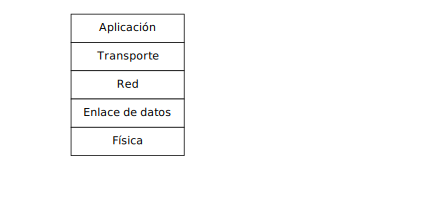
\includegraphics{arquitectura_tcpip}
\decoRule
\caption[Arquitectura TCP/IP]{Arquitectura TCP/IP.}
\label{fig:arquitectura_tcpip}
\end{figure}

Esta arquitectura se forma por cinco capas, y cada capa incluye varios
protocolos que les proporcionan servicios a los protocolos de la capa inmediata
superior. Las funciones que cumple cada una de las capas son los siguientes:

\keyword{Capa de aplicación} -- Contiene protocolos que ofrecen servicios
directamente a los usuarios. Estos servicios incluyen correo electrónico,
consulta de páginas \textit{web}, compartir archivos, telefonía, etc. Ejemplos:
HTTP, SMTP, FTP, SSH, etc.

\keyword{Capa de transporte} -- Es responsable de garantizar una transmisión
confiable de los datos, además del control de flujo de datos y el control de
congestión de la red. Ejemplos: TCP, UDP.

\keyword{Capa de red} -- Determina las rutas que deben seguir los paquetes de
información y se encarga de que cada uno siga su ruta hasta su destino. Sin
embargo, no garantiza la entrega de los paquetes. Los nodos más importantes en
esta capa son los enrutadores. Ejemplos: IP, BGP, RIP, OSPF, etc.

\keyword{Capa de enlace} -- Esta capa se encarga de las transmisiones de
paquetes entre nodos conectados directamente mediante un enlace. Dependiendo
del protocolo, puede ser un servicio confiable o no. Ejemplos: Ethernet, Wi-Fi,
Bluetooth, etc.

\keyword{Capa física} -- Convierte los paquetes en señales que se puedan
propagar por un medio físico y las transmite de un nodo a otro. Ejemplos: fibra
óptica, alambre de cobre, ondas de radiofrecuencia, etc.

Para que un protocolo pueda proporcionar su servicio a los de la capa superior,
se aplica un proceso que se conoce como encapsulamiento. Cuando el protocolo
que proporciona el servicio recibe un paquete del que lo solicita, le agrega su
propia cabecera al principio (también al final en algunos protocolos). De este
modo, cuando llega al nodo correspondiente, este extrae la cabecera para
analizarla y saber qué hacer con el paquete \cite{Kurose2013}.

%-----------------------------------
%   AUTOCONFIGURACIÓN DE DIRECCIONES
%-----------------------------------
\chapter{Autoconfiguración de direcciones en redes descentralizadas}

\label{ch:autoconfiguracion_de_direcciones_en_redes_descentralizadas}

Antes de que cualquier dispositivo pueda comunicarse a través de una red,
necesita tener asignada una dirección. Una dirección es un número que identifica
a un nodo dentro de una red. Cuando un paquete va destinado a una dirección,
ésta tiene que estar asignada a un solo dispositivo, de otro modo, no habría
manera de saber a cuál va dirigido.

La configuración manual consiste en que una persona configure la dirección.
Sin embargo, al requerir la intervención humana, es un proceso muy lento.
Este método resulta especialmente inconveniente cuando se trata de dispositivos
móviles, ya que estos dispositivos están diseñados para conectarse y
desconectarse con frecuencia en diferentes redes inalámbricas.

En las redes de infraestructura fija, la configuración de los nodos es
realizada, por lo general, por un servidor \textit{Dynamic Host Configuration
Protocol} (DHCP), que conoce las direcciones que están siendo ocupadas por todos
los nodos. Cuando un nodo se quiere unir a la red, contacta al servidor DHCP para
solicitarle una dirección IP, y éste le ofrece una dirección disponible
\cite{Kurose2013}. Este método es efectivo en una red de infraestructura fija,
ya que todos los nodos pueden contactar a través del enlace local al servidor
DHCP. En un MANET, la única manera que tendrían la mayoría de los nodos para
contactar a un servidor DHCP sería a través de nodos intermedios, que tienen la
libertad de moverse sin ninguna restricción. Por esta razón, no es factible que
un servidor DHCP se encargue de la configuración de direcciones en una red
descentralizada.

En las MANETs, los protocolos de autoconfiguración de direcciones son
responsables de asignar la dirección a cada nodo, garantizando su unicidad. A
continuación, se presentan los tipos de protocolos de autoconfiguración de
direcciones que se han desarrollado, así como algunos de los protocolos más
representativos de cada uno.

En este capítulo, se presenta el protocolo IPv6, que es el que rige el
funcionamiento de la retransmisión de paquetes, y especifica el formato de las
direcciones. Posteriormente, se presentan diferentes protocolos que se han
propuesto para la configuración autmática de direcciones para MANETs.

%-----------------------------------
%   PROTOCOLO IPV6
%-----------------------------------
\section{Protocolo IPv6}

\label{sec:protocolo_ipv6}

El protocolo \textit{Internet Protocol} (IP)\footnote{Protocolo de Internet.}
forma parte de la capa de red, y es el que rige la retransmisión de paquetes
a través de los enrutadores para que lleguen a su destino. Este protocolo
especifica en cada paquete cuál es el nodo de origen y cuál es el nodo de
destino (también llamado datagrama). Cada nodo se identifica de manera única
mediante un número llamado \keyword{dirección IP}. Cuando un enrutador obtiene
la dirección de destino de un paquete, consulta la mejor ruta y lo retransmite
al siguiente \cite{Kurose2013}.

La versión IPv4 fue desarrollada a principios de la década de 1970, y ha tenido
la hegemonía en la Internet durante más de 30 años. Pero desde hace más de dos
década se ha hecho cada vez más evidente su obsolescencia. Su limitación más
importante es que la cantidad de direcciones que ofrece ya se ha visto rebasada
por la cantidad de usuarios de Internet en el mundo \cite{Hagen2006}.

En 1993, se comenzó a desarrollar la versión IPv6, considerando las debilidades
de la versión anterior. La más importante mejora se encuentra en el tamaño de
las direcciones, ya que ofrece un espacio de direcciones más que suficiente
para identificar a todos los dispositivos del mundo, a diferencia de su
predecesor \cite{Hagen2006}.

%-----------------------------------
%   DATAGRAMA IPV6
%-----------------------------------
\subsection{Datagrama IPv6}

\label{subsec:datagrama_ipv6}

En la capa de red, la unidad de datos del protocolo se conoce como datagrama.
En el protocolo IPv6, un datagrama tiene una cabecera que contiene información
que los enrutadores analizan para realizar el enrutmaiento.En la figura
\ref{fig:formato_datagrama_ipv6_general} se muestra el formato de un datagrama
IPv6 \cite{Hagen2006}.

\begin{figure}[th]
\centering
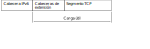
\includegraphics{formato_datagrama_ipv6_general}
\decoRule
\caption[Datagrama IPv6]{Formato de un datagrama IPv6.}
\label{fig:formato_datagrama_ipv6_general}
\end{figure}

El formato de la cabecera IPv6 se muestra en la figura
\ref{fig:formato_cabecera_ipv6}, y se forma por los siguientes campos
\cite{RFC2460}:

\begin{figure}[th]
\centering
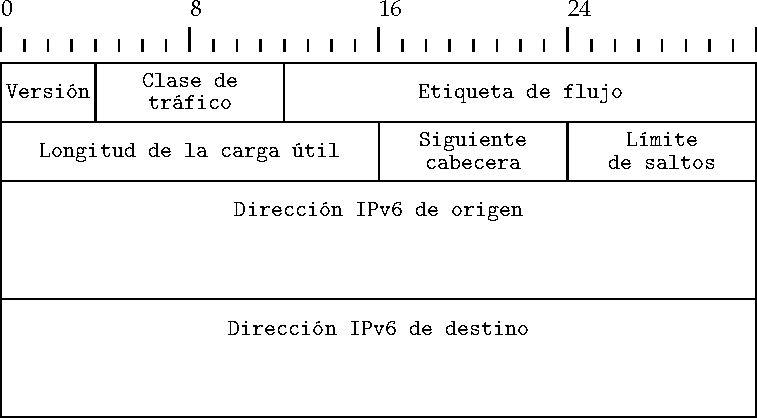
\includegraphics{formato_cabecera_ipv6}
\decoRule
\caption[Cabecera IPv6]{Formato de la cabecera IPv6.}
\label{fig:formato_cabecera_ipv6}
\end{figure}

\keyword{Versión (4 bits)} -- Versión del protocolo IP.

\keyword{Clase de tráfico (1 byte)} -- Prioridad asignada al datagrama.

\keyword{Etiqueta de flujo (20 bits)} -- Identificar una secuencia de
datagramas.

\keyword{Longitud de carga útil (2 bytes)} -- Número de bytes de la carga útil.

\keyword{Siguiente cabecera (1 byte)} -- Identifica el tipo de cabecera que
sigue después de la cabecera IPv6.

\keyword{Límite de saltos (1 byte)} -- Número de veces que se ha
retransmitido el datagrama. Es decrementado por cada enrutador que lo
retransmite. Si llega a cero, se descarta el datagrama.

\keyword{Dirección IPv6 de origen (16 bytes)} -- Dirección IPv6 del dispositivo
que originó el datagrama.

\keyword{Dirección IPv6 de destino (16 bytes)} -- Dirección IPv6 del dispositivo
al que va dirigido el datagrama.

%-----------------------------------
%   DIRECCIONAMIENTO IPV6
%-----------------------------------
\subsection{Direccionamiento IPv6}

\label{subsec:direccionamiento_ipv6}

Una dirección IP es un número que identifica de manera única cada interfaz de
red de un dispositivo. Comúnmente se asocia la dirección IP con el dispositivo.
Sin embargo, si un dispositivo tiene más de una interfaz, puede tener más de una
dirección IP. Incluso una sola interfaz puede tener asignadas varias
direcciones.

En la dirección se encuentra la información de la red a la que está conectada la
interfaz, así como el identificador único de la interfaz dentro de esa red. Con
esta estructura jerárquica, cuando se enruta un paquete hacia su destino, el
primer objetivo es que el paquete llegue a la red correspondiente. Una vez que
el paquete llega a la red, se hace un enrutamiento local para que llegue al
nodo correspondiente \cite{Kurose2013}.

En el protocolo IPv6, las direcciones tienen una longitud de 128 bits. Con un
espacio de direcciones de tamaño $2^128$, se cuenta con suficientes para asignar
una (o más si fuera necesario) a cada dispositivo que existe. Esta fue la
principal motivación de la creación del protocolo IPv6, aunque incluye muchas
otras mejoras respecto a IPv4 \cite{Hagen2006}.

Una dirección IPv6 se divide en ocho bloques de 16 bits, que se representan en
notación hexadecimal y se separan con \code{:}. Cuando hay una secuencia de
bloques que contiene únicamente ceros, se puede comprimir usando \code{::}. Por
ejemplo:

\noindent\code{2001:DB8:0:0:202:B3FF:FE1E:8329}\\
\code{2001:DB8::202:B3FF:FE1E:8329}

La notación de prefijo se usa para representar un bloque del espacio de
direcciones. Por ejemplo:

\noindent\code{2E78:DA53:1200::/40}

Este prefijo representa todas las direcciones posibles que comienzan con
los primero 40 bits de la dirección \code{2E78:DA53:1200::}. Generalmente, el
prefijo corresponde al identificador de la red; sin embargo, hay prefijos que
tienen significados especiales \cite{Hagen2006}.

El protocolo IPv6 define tres tipos de direcciones \cite{CiscoIpv62011}:

\keyword{\textit{Unicast}} -- Identifica una única interfaz en un nodo. Los
paquetes que se envían a una dirección \textit{unicast} son entregados
solamente a dicha interfaz.

\keyword{\textit{Anycast}} -- Una dirección \textit{anycast} puede ser asignada
a interfaces de diferentes nodos. Los paquetes dirigidos a una dirección de este
tipo sólo llegan a la interfaz más cercana que tenga asignada la dirección,
según los protocolos de enrutamiento.

\keyword{\textit{Multicast}} -- Es un identificador para un conjunto de
interfaces, que generalmente pertenecen a nodos distintos. Cuando un paquete
se envía a una dirección \textit{multicast}, éste llega a todas las interfaces
que pertenecen al gurpo.


%-----------------------------------
%   AUTOCONFIGURACIÓN DE DIRECCIONES CON ESTADO
%-----------------------------------
\section{Autoconfiguración de direcciones con estado}

\label{sec:autoconfiguracion_de_direcciones_con_estado}

El protocolo DHCP es el ejemplo más claro de este tipo de protocolos. Se dice
que es con estado debido a que mantiene en todo momento el registro de todos los
nodos que formar parte de la red y la dirección de cada uno. A pesar de que este
enfoque tiene una aplicación limitada en las MANETs, se han desarrollado
métodos de configuración con estado para este tipo de redes. Estos se basan,
principalmente, en la distribución y administración de las direcciones entre un
grupo de nodos de manera descentralizada \cite{Grajzer2019}.

El protocolo MANETconf \cite{Nesargi2002} es uno de los más representativos de
esta categoría. En este protocolo, todos los nodos tienen el registro de todas
las direcciones que se han asignado en la red. Cuando un nuevo nodo, denominado
\textit{solicitante}, quiere unirse a una red, contacta a un nodo que tenga a su
alcance, llamado \textit{iniciador}. En iniciador envía una solicitud al resto
de los nodos para saber si una dirección está disponible. Cuando recibe una
respuesta positiva de todos los demás nodos, le puede asignar la dirección al
solicitante. Después, el iniciador envía la notificación de que la dirección ya
se encuentra en uso al resto de los nodos. Este protocolo tiene varias
desventajas, como la necesidad de que todos los nodos cuenten con espacio para
almacenar todas las direcciones en uso, así como un alto uso de los recursos de
la red, ya que se tiene que inundar con solicitudes y notificaciones cada vez
que se une un nuevo nodo.

Un método para reducir el problema de la sobrecarga de la red que presenta el
protocolo MANETconf, es propuesto por Munjal \textit{et al.} \cite{Munjal2014},
en el que el iniciador no espera confirmaciones de todos los demás nodos cuando
envía una solicitud. Cuando un nodo recibe la respuesta del iniciador, éste
responde únicamente si tiene que avisarle que la dirección se encuentra en uso.
Esto reduce significativamente el uso de los recursos de la red, sin embargo,
aún se debe inundar con una solicitud cuando un iniciador necesita asignar una
dirección. Además, como en el protocolo MANETconf, los nodos deben tener la
lista de todas las direcciones en uso.

El protocolo \textit{Mobile Agents based Address Auto-Configuration}
(MAAC)\footnote{Autoconfiguración de direcciones basada en agentes móviles.} fue
propuesto por Korichi \textit{et al.} \cite{Korichi2018}. En este protocolo,
los nodos de la red se organizan jerárquicamente en grupos, y cada grupo es
administrado por un agente móvil alojado en uno de los nodos. Este sistema
móvil multi-agente forma servidor virtual como sustituto de un servidor DHCP.
Cuando un nodo se quiere unir a la red, envía una solicitud de dirección a los
nodos cercanos, y cada uno reenvía la solicitud al agente que lo configuró. Si
un agente recibe la solicitud, responde con una propuesta de de dirección. El
nodo que originó la solicitud úicamente considera la propuesta del agente que
está a menos saltos de distancia.

Este tipo de protocolos tienen el inconveniente de requerir el mantenimiento de
las tablas con las direcciones de todos los nodos de la red, cuyo tamaño
incrementa confome se incorporan nuevos nodos. Esto hace que, mientras más
grande se hace la red, se necesitan más recursos, tanto computacionales como de
comunicación.

%-----------------------------------
%   AUTOCONFIGURACIÓN DE DIRECCIONES SIN ESTADO
%-----------------------------------
\section{Autoconfiguración de direcciones sin estado}

\label{sec:autoconfiguracion_de_direcciones_sin_estado}

En la configuración automática sin estado, cada nodo se asigna su propia
dirección, y no necesita mantener información de las direcciones de todos los
demás nodos. En general, para que un nuevo nodo pueda obtener una dirección, se
lleva a cabo un proceso llamado \textit{Duplicate Address Detection}
(DAD)\footnote{Detección de direcciones duplicadas.}. Cuando un nodo quiere
unirse a la red, envía una consulta con una dirección tentativa a todos los
demás nodos. Si alguno ya tiene asignada esta dirección, le envía una
notificación al nodo nuevo, y este repite este proceso. Si no recibe ninguna
respuesta dentro de un intervalo de tiempo, asume que la dirección está
disponible y puede usarla \cite{Grajzer2019}.

El protocolo \textit{Address Reservation and Optimistic Duplicated address
detection} (AROD)\footnote{Resesrvación de direcciones y detección optimista de
direcciones suplicadas.} propuesto por Kim \textit{et al.} \cite{Kim2007}
funciona mediante la reservación de direcciones, lo que reduce el tiempo de
configuración y el uso del ancho de banda de la red. Este protocolo define tres
tipos de nodos:
\begin{enumerate*}[label=\arabic*)]
  \item un nodo que tiene reservada una dirección además de su propia dirección;
  \item un nodo que no tiene ninguna dirección reservada;
  \item un nuevo nodo
\end{enumerate*}.
Cuando un nuevo nodo quiere entrar a la red, selecciona uno de sus vecinos
como agente, que se encarga de asignarle una dirección. Si el agente es de tipo
1, le asigna la dirección reservada inmediatamente. Si el agente es de tipo 2,
le solicita la dirección reservada a otro nodo de tipo 1. Esta operación
resulta más eficiente que el procedimiento DAD, ya que requiere un único
mensaje \textit{broadcast}.

Después de la configuración de un nuevo nodo, el agente selecciona dos
direcciones al azar, y realiza la operación DAD para cada una. Si ambas
direcciones son únicas, el agente reserva una y el nuevo nodo reserva otra, y
ambos nodos son de tipo 1. Si una dirección está ocupada, al agente reserva la
dirección libre, y el nuevo nodo es de tipo 2. Si ninguna dirección está
disponible, tanto el agente como el nuevo nodo son de tipo 2. Este protocolo
requiere baja demanda de comunicación de la red, además de que garantiza que
las direcciones son únicas.

En \cite{Munjal2015}, Mujal presenta el protocol \textit{Scalable
Hierarchical Distributive Auto-Configuration Protocol} (
SHDACP-IPv6)\footnote{Protocolo de autoconfiguración distributiva jerárquica
escalable.}.
En este protocolo, las direcciones IPv6 se componen de cinco campos, como se
ilustra en la figura \ref{fig:formato_direccion_shdacp}: prefijo (7 bits),
identificador global (41 bits), identificador de partición (16 bits),
identificador de grupo (48 bits) e identificador de red (16 bits).

\begin{figure}[th]
\centering
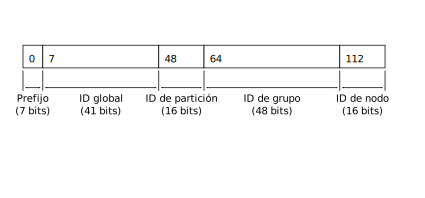
\includegraphics{formato_direccion_shdacp}
\decoRule
\caption[Formato de las direcciones del protocolo SHDACP-IPv6]{Formato de las
direcciones del protocolo SHDACP-IPv6\protect\footnotemark.}
\label{fig:formato_direccion_shdacp}
\end{figure}

\footnotetext{Adaptación del esquema presentado por Mujal \cite{Munjal2015}.}

Cuando un nodo, denominado \textit{solicitante}, se quiere unir a una red,
transmite un mensaje \textit{Neighbor\_Query}, esperando recibir como respuesta
al menos un mensaje \textit{Neighbor\_Reply} de otro nodo ya configurado. Si no
recibe respuesta, repite el proceso. Después de cierta cantidad de intentos, si
no recibe respuesta, el solicitante asume que es el primer nodo de la red, y se
autoconfigura como \textit{Cluster Head} (CH), o cabeza de grupo, con un número
de partición aleatorio, un número de grupo aleatorio y el identificador de nodo
1. Cuando otro nodo se quiere unir a la red, el CH recibe una solicitud de
éste, y le asigna un identificador de nodo secuencialmente. Si un nuevo nodo se
encuentra a más de cierto número de saltos de distancia de todos los CHs, se
autoconfigura como un nuevo CH.

Este protocolo también cuenta con mecanismos para lidiar con particiones de la
red, causadas por el movimiento impredecible de los nodos, así como para
combinar dos o más particiones. Sin embargo, no garantiza que no existan
direcciones repetidas, pero gracias al amplio espacio de direcciones que ofrece
el protocolo IPv6, la probabilidad de que esto ocurra es casi nula.

El protocolo IPv6 especifica un procedimiento cuyo propósito es ayudar a
llevar a cabo la autoconfiguración de direcciones sin estado, llamado
\textit{Neighbor Discovery} (ND)\footnote{Descubrimiento de vecinos.}. Cuando un
nodo quiere obtener una dirección, envía un mensaje \textit{Neighbor Solicitation}
(NS), o solicitud de vecino, a sus vecinos directos. Si alguno ya tiene asignada
la dirección, responde con un mensaje \textit{Neighbor Advertisement} (NA), o
anuncio de vecino. Sin embargo, este procedimiento no se puede aplicar en una
MANET, ya que funciona únicamente dentro del alcance del enlace local.

Grajzer \textit{et al.} \cite{Grajzer2019} proponen ND++, una extensión del
estándar ND que agrega dos tipos de mensajes: \textit{multihop Neighbor
Solicitation} (mNS), o solicitud de vecino multi-salto, y \textit{multihop
Neighbor Advertisement} (mNA), o anuncio de vecino multi-salto. Cuando un nodo
realiza el procedimiento DAD y determina que su dirección no está en uso por
sus vecinos directos, ejecuta el procedimiento DAD++, en el que inunda la red
con un mensaje mNS, esperando como respuesta un mensaje mDA. ND++ usa una
técnica de optimización de inundación que sólo requiere conocer los vecinos que
se encuentran hasta dos saltos de distancia de cada nodo, limitando el
intercambio de mensajes de control necesarios únicamente al enlace local.

\chapter{Protocolos de enrutamiento}
%-----------------------------------
%   PROTOCOLOS DE ENRUTAMIENTO
%-----------------------------------
\label{ch:protocolos_de_enrutamiento}

Los protocolos de enrutamiento se encargan de determinar las rutas que deben
seguir los datagramas para llegar a su destino. En las redes de
infraestructura fija, la topología cambia muy poco, por lo que es raro que las
rutas tengan que modificarse. Sin embargo, en la sección \ref{ch:vanets} vimos
que una de las características de las VANETs es que la topología cambia todo el
tiempo. Esto hace que la vigencia de las rutas sea muy corta, por lo que se
necesitan protocolos de enrutamiento que puedan lidiar con estos problemas.

En este capítulo, se explica cómo se almacenan las rutas y cómo se usan para
retransmitir los datagramas de nodo a nodo. Después, se presentan diferentes
enfoques de enrutamiento para redes descentralizadas, y algunos de los
protocolos que se han propuesto.

\section{Tablas de enrutamiento}
%-----------------------------------
%   TABLAS DE ENRUTAMIENTO
%-----------------------------------
\label{sec:tablas_de_enrutamiento}

Generalmente, cuando un dispositivo debe transmitir un paquete de información,
el destinatario no se encuentra inmediatamente alcanzable a través de un sólo
enlace. El paquete debe seguir una ruta, que es una secuencia de enlaces entre
dispositivos mediante los cuales se puede llegar de un nodo a otro. Los
enrutadores son dispositivos que reciben datagramas y cuya función es
retransmitirlos por el siguiente enlace de la ruta.

Para saber hacia dónde debe retransmitir un datagrama, cada enrutador tiene una
\textbf{tabla de enrutamiento}, donde cada registro contiene los siguientes
datos \cite{Hagen2006}:

\keyword{Prefijo IPv6 y longitud del prefijo} -- Prefijo relevante de la
dirección.

\keyword{Dirección del siguiente salto} -- Dirección IPv6 de la interfaz del
siguiente salto.

\keyword{Interfaz del siguiente salto} -- Interfaz del enrutador que se usa para
llegar al siguiente enrutador a lo largo de la ruta.

\keyword{Métrica} -- Número que indica la distancia total hasta el destino.

\keyword{Temporizador} -- Tiempo desde el que se actualizó por última vez la
la ruta.

\keyword{Fuente de la ruta o protocolo} -- Entidad que proporcionó la
información de la ruta. Por ejemplo, puede ser una ruta configurada manualmente
o por un protocolo.

Cuando un enrutador recibe un datagrama, extrae de la cabecera la dirección de
destino. Para cada registro de la tabla de enrutamiento, compara el prefijo
indicado en la ruta con el prefijo de la dirección de destino del datagrama
hasta encontrar una coincidencia. Siempre se comienza con los prefijos más
largos. Una vez que se encontró el registro correspondiente, se decrementa en 1
el valor del límete de saltos del datagrama IPv6, y se retransmite hacia el
enrutador correspondiente. Si no se encuentra ninguna coincidencia en la tabla,
se descarta el datagrama.

Aunque las tablas de enrutamiento se pueden llenar manualmente, en la práctica
se utilizan protocolos de enrutamiento para hacerlo. Los protocolos de
enrutamiento consisten en el intercambio de información entre los enrutadores
que sirve para determinar las rutas y llenar las tablas de enrutamiento.

\section{Enrutamiento basado en la topología}
%-----------------------------------
%   ENRUTAMIENTO BASADO EN LA TOPOLOGÍA
%-----------------------------------
\label{sec:enrutamiento_basado_en_la_topologia}

El enrutamiento basado en la topología es ideal para las redes de
infraestructura fija, ya que los cambios en la topología son muy raros en este
tipo de redes. No obstante, se han diseñado protocolos para redes móviles con
este enfoque. Existen principalmente dos técnicas usadas en este tipo de
enrutamiento, que se describen a continuación.

\subsection{Enrutamiento proactivo}
%-----------------------------------
%   ENRUTAMIENTO PROACTIVO
%-----------------------------------
\label{subsec:enrutamiento_proactivo}

Los protocolos de enrutamiento proactivos se caracterizan porque mantienen
siempre actualizadas las rutas hacia todos los demás nodos, sean requeridas o
no. De esta manera, cuando se necesita retransmitir un datagrama, la ruta está
disponible en la tabla de enrutamiento \cite{Wenden2005}.

El protocolo \textit{Destination-Sequenced Distance-Vector}
(DSDV)\footnote{Vector de distancias por secuencia de destinos.} desarrollado
por Perkins \textit{et al.} \cite{Perkins1994}, es un protocolo proactivo en el
que cada nodo tiene conoce las rutas hacia todos los demás nodos, así como la
cantidad de saltos que se necesitan para llegar a cada uno. Cada registro de la
tabla de enrutamiento tiene un número de secuencia para saber cuáles son las
rutas más nuevas.

En este protocolo, cada nodo transmite periódicamente actualizaciones de su
tabla de enrutamiento mediante mensajes \textit{broadcast}. No obstante, para
reducir el tráfico en la red, existen dos tipos de actualizaciones que los
nodos pueden transmitir: actualizaciones de la tabla de enrutamiento completa,
que se transmiten cuando hay cambios importantes en las rutas, y actualizaciones
de cambios menores, que son los que se transmiten más comúnmente.

\subsection{Enrutamiento reactivo}
%-----------------------------------
%   ENRUTAMIENTO REACTIVO
%-----------------------------------
\label{subsec:enrutamiento_reactivo}

El enrutamiento reactivo, también conocido como enrutamiento bajo demanda,
consiste en buscar una ruta hacia únicamente si es necesario. La principal
ventaja que tienen los protocolos reactivos sobre los proactivos es que no se
necesita usar recursos de la red para descubrir rutas que no son necesarias.
Pero, por otro lado, los paquetes sufren demoras debido a que se debe esperar
hasta que la ruta sea descubierta para poder transmitirlos \cite{Wenden2005}.

En el protocolo \textit{Dynamic Source Routing} (DSR)\footnote{Enrutamiento de
origen dinámico.} \cite{Johnson1996}, se construye una \textit{ruta de origen}
que se incluye dentro de la cabecera del paquete. La ruta de origen contiene
las direcciones de todos los nodos por los que debe pasar el paquete para llegar
a su destino. El remitente transmite el paquete al primer nodo indicado en la
ruta de origen; cuando éste lo recibe, lo retransmite al siguiente nodo
indicado en la ruta de destino, a menos que sea el nodo de destino.

Cada nodo tiene una \textit{caché de rutas} donde almacena todas las rutas de
origen que ha aprendido. Cuando se necesita enviar un paquete y no se encuentra
una ruta en la caché de rutas, se usa el procedimiento de \textit{descubrimiento
de ruta}, en el que envía un mensaje de \textit{solictud de ruta}. Este mensaje
es retransmitido por los demás nodos hasta llegar al nodo de destino, o hasta
llegar a un nodo que tenga una ruta al destinatario requerido. Cada vez que un
nodo retransmite la solicitud de ruta, agrega su dirección al paquete para
tener un registro de los nodos por los que pasó para llegar al destino.

Este protocolo también tiene un procedimiento de \textit{mantenimiento de
rutas}, en el que, cuando se detecta que se perdió un enlace, se disemina un
mensaje de \textit{error de ruta}. Cuando un nodo recide este tipo de mensajes,
truca las rutas que contenían ese enlace.

Otro protocolo proactivo es \textit{Ad hoc On-demand Distance-Vector}
(AODV)\footnote{Vector de distancias \textit{ad hoc} bajo demanda.}
\cite{Perkins1999}. En este protocolo, los nodos que no pertenezcan a una ruta
activa no participan en el intercambio de información sobre el enrutamiento.
Además, los nodos no tienen que mantener ni descubrir rutas si no es necesario.
El proceso del descubrimiento de rutas es similar al del protocolo DSR. Sin
embargo, AODV usa tablas de enrutamiento tradicionales para almacenar las
rutas. También usa números de secuencia, como el protocolo DSDV, para prevenir
bucles en las rutas y saber qué rutas son más viejas que otras.

\section{Enrutamiento basado en la posición}
%-----------------------------------
%   ENRUTAMIENTO BASADO EN LA POSICIÓN
%-----------------------------------
\label{sec:enrutamiento_basado_en_la_posicion}

En los protocolos de enrutamiento basados en la topología, es necesario
conocer, de manera parcial o total, los enlaces entre los nodos de la red. En
el enrutamiento basado en la posición, las decisiones de retransmisión de
paquetes se toman con base en la ubicación del destinatario y de los vecinos.
Es por esto que es más eficiente este enfoque en las redes que tienen cambios en
la topología muy frecuentemente, como las VANETs. \cite{Wenden2005}

En este tipo de enrutamiento, no se puede transmitir un paquete si no se conoce
la ubicación del destinatario. Para esto, es necesario contar con un servicio de
localización. No obstante, como en el caso del servicio de autoconfiguración de
direcciones, debe ser un servicio descentralizado, por lo que todos o un
subconjunto de los nodos participan en él \cite{DeMoraisCordeiro2006}.

Las primeras dos subsecciones siguientes están basadas en el estudio sobre
enrutamiento basado en la posición realizado por Mauve \textit{et al.} en
\cite{Mauve2001}. Primero, se presentan los principales tipos de servicios de
localización para MANETs. Después, se muestran diferentes protocolos de
enrutamiento que utilizan diversos criterios para retransmitir un paquete. Por
último, se exponen diferentes protocolos específicos para VANETs.

\subsection{Servicios de localización}
%-----------------------------------
%   SERVICIOS DE LOCALIZACIÓN
%-----------------------------------
\label{subsec:servicios_de_localizacion}

Un servicio de localización permite a un nodo consultar la ubicación de otro
cuando necesita enviarle algún mensaje a través de la red. En general, en una
red \textit{ad hoc} no se puede asumir que se puede instalar un servidor
centralizado que se pueda contactar inequívocamente por cualquier nodo, como en
las redes de infraestructura fija. Por la naturaleza de este tipo de redes, debe
ser un servicio distribuido entre varios nodos. El servicio puede estar
constituido por todos los nodos o sólo algunos, y cada uno des estos puede
tener disponible la ubicación de todos los nodos únicamente de algunos
\cite{DeMoraisCordeiro2006}.

En el protocolo \textit{Distance Routing Effect Algorithm for Mobility}
(DREAM)\footnote{Algoritmo de enrutamiento de efecto de distancia para
movilidad} diseñado por Basagni \textit{et al.} \cite{Basagni1998}, se
especifica un servicio de localización en el que cada nodo sabe la posición de
todos los demás nodos. Esto se logra haciendo que cada nodo transmita
actualizaciones de su ubicación constantemente. Sin embargo, para reducir la
saturación de la red, los nodos que se mueven más lento, transmiten menos
frecuentemente sus actualizaciones.

\begin{figure}[th]
\centering
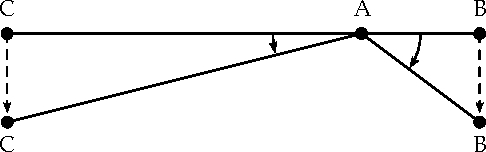
\includegraphics{efecto_distancia}
\decoRule
\caption[Efecto de distancia]{Efecto de distancia\protect\footnotemark.}
\label{fig:efecto_distancia}
\end{figure}

\footnotetext{Adaptación del esquema presentado por Mauve \cite{Mauve2001}.}

Este protocolo también aprovecha el \textit{efecto de distancia} para reducir el
alcance de las actualizaciones. En la figura \ref{fig:efecto_distancia} se
muestra el efecto de distancia. El nodo A se considera estático, y los nodos B
y C se mueven la misma distancia y en la misma dirección. No obstante, desde la
perpectiva del nodo A, el nodo B tuvo un movimiento más significativo que el
nodo C. Por esta razón, el nodo A requiere actualizaciones de la ubicación del
nodo B con más frecuencia que del nodo C.

En \cite{Haas1999}, se propone un servicio de localización llamado
\textit{Uniform Quorum Systems} (UQS)\footnote{Sistemas de \textit{quorum}
uniformes.}, en el que las actulizaciones de ubicación van dirigidas a un
subconjunto de los nodos, llamado \textit{quorum}, y las peticiones pueden
ser referidas a un \textit{quorum} potencialmente diferente. Cuando la
intersección entre dos \textit{quorums} diferentes no es vacía, se garantiza
que se encontrará un versión actualizada de la ubicación.

En el ejemplo de la figura \ref{fig:quorum}, los nodos 1-6 son seleccionados
para conformar el servicio de localización; este subconjunto de nodos se
denomina \textit{backbone virtual}. El nodo D envía su posición al nodo 6,
que es el nodo perteneciente el \textit{backbone} virtual más cercano. El nodo
6 selecciona el \textit{quorum} A, que contiene los nodos 1, 2 y 6, para
almacenar la actualización del nodo D. El nodo S envía una solicitud al nodo 4
para obtener la ubicación del nodo D. Este selecciona el \textit{quorum} B,
formado por los nodos 4, 5 y 6, para consultar la ubicación.

\begin{figure}[th]
\centering
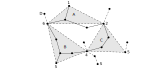
\includegraphics{quorum}
\decoRule
\caption[Ejemplo de \textit{quorum}]{Ejemplo de \textit{quorum}\protect\footnotemark.}
\label{fig:quorum}
\end{figure}

\footnotetext{Adaptación del esquema presentado por Mauve \cite{Mauve2001}.}

Otro servicio de localización es \textit{Grid Location Service}
(GLS)\footnote{Servicio de localización de cuadrícula.} \cite{Li2000}. En este
caso, la región donde se encuentra la red se divide de manera jerárquica en
cuadrados. Cuatro cuadrados de orden $n$ están contenidos dentro de un cuadrado
de orden $n+1$; cuatro cuadrados de orden $n+1$ están contenidos dentro de un
cuadrado de orden $n+2$, y así sucesivamente según se necesite.

El funcionamiento de GLS se muestra en la figura \ref{fig:gls}. Para determinar
cómo se almacena la posición de un nodo, se introduce el concepto de
\textit{nodo de ID cercano}, que se define de la siguiente manera: dado el
identificador de un nodo, su nodo de ID cercano el tiene el identificador mayor
más cercano al suyo entre los nodos que se encuentran dentro de un cuadrado. En
este ejemplo, el nodo 10 envía su ubicaión al nodo de ID cercano de cada uno de
los tres cuadrados circundantes de primer orden, que son los nodos 15, 18 y 73,
así como a todos los nodos que se encuentran dentro de su mismo cuadrado. En
cada uno de los tres cuadrados vecinos de segundo orden, también se selecciona
el nodo de ID cercano para compartirles su ubicación, que son los nodos 14, 25
y 29, como se muestra en la figura \ref{fig:gls1}. Este procedimiento se sigue
hasta cubrir toda el área de la red.

Si suponemos que el nodo 78 necesita conocer la ubiación del nodo 10, este debe
localizar y contactar a un nodo cercano que le pueda proporcionar ese dato. En
este caso, se trata del nodo 29. Así como el nodo 10 compartió su ubicación con
sus nodos de ID cercano, el nodo 29 compartió su ubicación con los nodos 36, 43
y 64. Hay que notar que, estos nodos automáticamente son nodos de ID cercano del
nodo 10 en su respectivo cuadrado, ya que también lo son del nodo 29. Por esto,
se puede rastrear el nodo 10 a través de una secuencia de identificadores de
nodos descendentes por cada uno de los cuadros de todos los órdenes. Es decir,
el nodo 78 obtiene del nodo 36 la ubicación del nodo 29 (orden 1), y obtiene
del nodo 29 la ubicación del nodo 10 (orden 2), como se observa en la figura
\ref{fig:gls2}.

\begin{figure}[th]
\centering

\begin{subfigure}[b]{\textwidth}
\centering
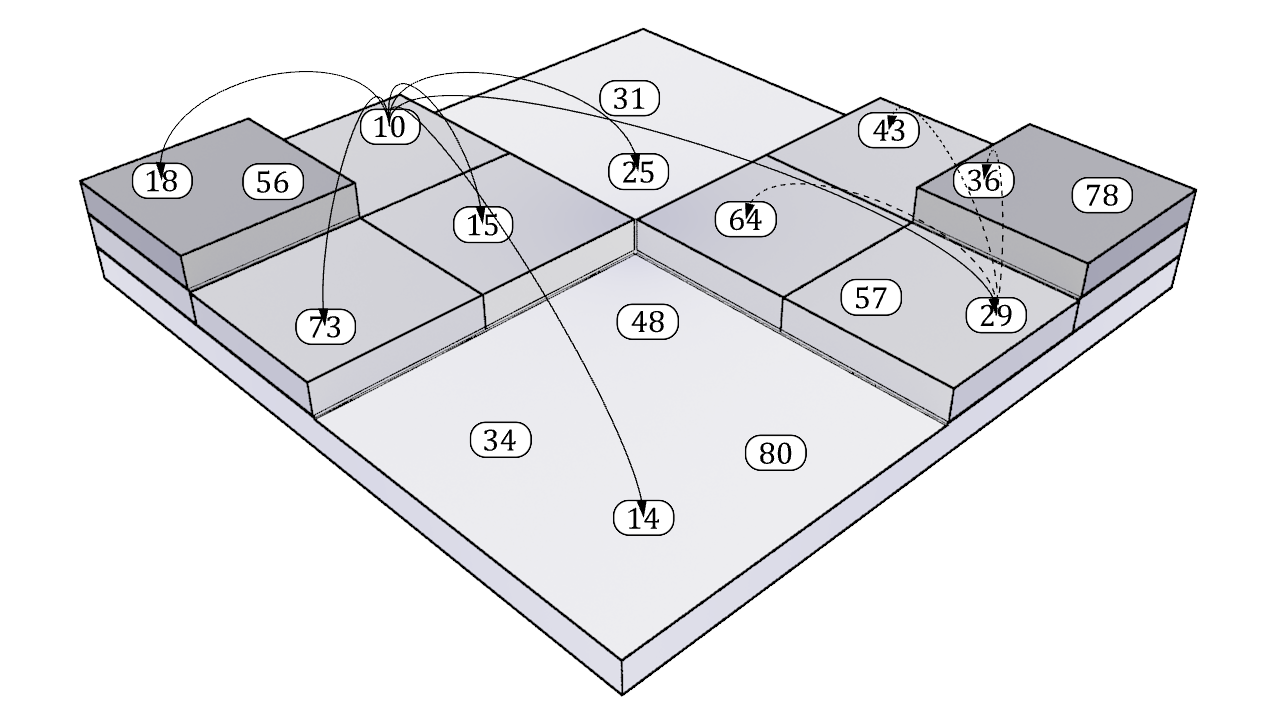
\includegraphics[scale=0.29]{gls1}
\caption{Almacenamiento de la ubicación de los nodos 10 y 29.}
\label{fig:gls1}
\end{subfigure}
\hfill
\begin{subfigure}[b]{\textwidth}
\centering
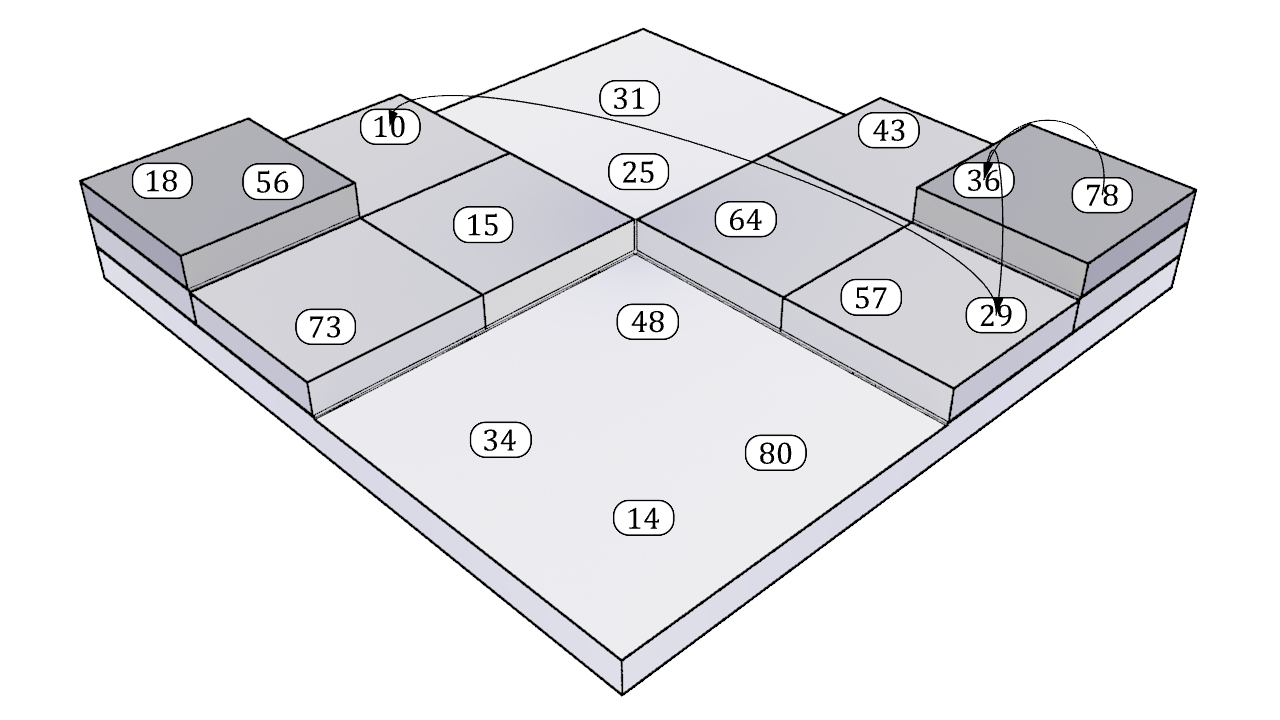
\includegraphics[scale=0.29]{gls2}
\caption{Descubrimiento de la ubicación del nodo 10 desde el nodo 78.}
\label{fig:gls2}
\end{subfigure}

\decoRule
\caption[Funcionamiento de GLS]{Funcionamiento de GLS\protect\footnotemark.}
\label{fig:gls}
\end{figure}

\footnotetext{Adaptación del esquema presentado por Mauve\cite{Mauve2001}.}

\subsection{Estrategias de retransmisión de paquetes}
%-----------------------------------
%   ESTRATEGIAS DE RETRANSMISIÓN DE PAQUETES
%-----------------------------------
\label{subsec:estrategias_de_retransmision_de_paquetes}

En esta sección se presentan algunos de los criterios que se consideran para la
retransmisión de paquetes a la hora de hacer el enrutamiento.

\subsubsection{Retransmisión voraz}
%-----------------------------------
%   RETRANSMISIÓN VORAZ
%-----------------------------------
\label{subsubsec:retransmision_voraz}

La retransmisión voraz consiste en considerar únicamente la información que se
tiene de manera inmediata para seleccionar hacia qué nodo retransmitir un
paquete. Ésta información, por lo general, es únicamente la ubicación del
destinatario y las de los vecinos que se encuentran dentro del área de cobertura. La
retransmisión se hace hacia alguno de los nodos que se encuentren más cerca del
destinatario, y este proceso se repite hasta que se llegue al destinatario.

\begin{figure}[th]
\centering
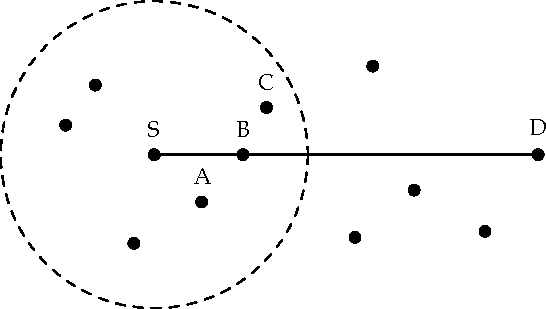
\includegraphics{retransmision_voraz}
\decoRule
\caption[Estrategias de retransmisión voraz]{Estrategias de retransmisión
voraz\protect\footnotemark.}
\label{fig:retransmision_voraz}
\end{figure}

\footnotetext{Adaptación del esquema presentado por Mauve\cite{Mauve2001}.}

Existen distintas maneras de seleccionar el siguiente salto. Estas se
ejemplifican en la figura \ref{fig:retransmision_voraz}, donde el nodo S es
el remitente y el nodo D es el destinatario. El círculo alrededor del nodo S
indica su radio máximo de transmisión. Uno de los criterios para seleccionar el
siguiente salto se seleccionar el vecino más cercano al destinatario. En el
ejemplo, este sería el nodo C. La idea es minimizar el número de saltos para
llegar al destino.

Otro método para seleccionar el siguiente salto es elegir el vecino más cercano
que se encuentre en la dirección del destinatario. En la figura
\ref{fig:retransmision_voraz}, este sería el nodo A. Este criterio es
conveniente si el nodo que retransmite es capaz de ajustar la potencia de la
transmisión, ya que se reduce la probabilidad de que existan colisiones con
otras transmisiones.

Otra regla que se puede seguir es seleccionar el vecino que esté más cercano a
la línea recta que une al remitente y al destinatario. En el ejemplo de la
figura \ref{fig:retransmision_voraz}, se trata del nodo B. El objetivo es
minimizar la distancia que viaja un paquete para llegar a su destino. También
es posible seleccionar aleatoriamente algún vecino que se encuentre más cerca
del destinatario. Esto reduce la precisión de la información requerida para
hacer la selección del siguiente nodo, además de que agiliza su selección, ya
que la cantidad de operaciones necesarias para esta operación es menor.

Por desgracia, la retransmisión voraz puede fallar cuando un nodo que va a
retransmitir un paquete está más cercano al destinatario que todos sus vecinos,
lo que se conoce como \textit{máximo local}. En este caso, no se podría
encontrar una ruta hacia el destinatario aunque exista al menos una. Esta
situación se ilustra en la figura \ref{fig:retransmision_voraz_falla}. En el
protocolo \textit{Greedy Perimeter Stateless Routing}
(GPSR)\footnote{Enrutamiento voraz y de perímetro sin estado.} propuesto por
Karp \textit{et al.} \cite{Karp2000}, cuando un paquete llega a un máximo
local, entra en un modo de recuperación cuyo criterio de retransmisión es
distinto al voraz, y regresa al modo voraz cuando llega a un nodo que está más
cercano al destinatario que el nodo donde entró al modo de recuperación.

\begin{figure}[th]
\centering
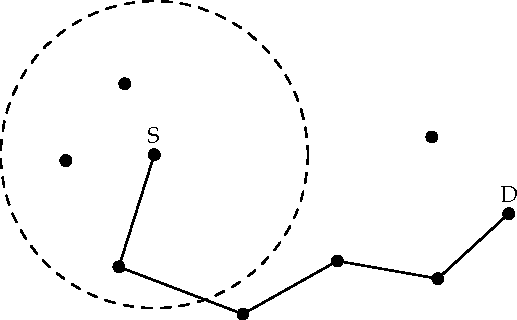
\includegraphics{retransmision_voraz_falla}
\decoRule
\caption[Falla en la retransmisión voraz]{Falla en la retransmisión
voraz\protect\footnotemark.}
\label{fig:retransmision_voraz_falla}
\end{figure}

\footnotetext{Adaptación del esquema presentado por Mauve\cite{Mauve2001}.}

El modo de recuperación del protocolo GPSR consiste en construir un subgrafo
plano con la ubicación de los vecinos y la del nodo que va a retransmitir el
paquete. La retransmisión se hace por el interior de las caras del subgrafo
usando la regla de la mano derecha. La figura \ref{fig:recuperacion_gpsr}
muestra cómo se usa el modo de recuperación para que un paquete llegue del nodo
S al nodo D. Se retransmite el paquete en la siguiente arista en el sentido
antihorario de la arista desde la que llegó. Cuando la arista tentativa de
retransmisión intersecta con la línea recta que une el remitente y el
destinatario, se verifica si esa intersección está más cerca del destinatario
que cualquier otra intersección encontrada anteriormente. Si este es el caso,
se cambia a la cara que está al otro lado de la arista tentativa, y se hace la
retransmisión por la siguiente arista en el sentido antihorario.

La cabecera del paquete contiene información para poder llevar a cabo el modo de
recuperacion, como la ubicación del nodo donde entró en este modo, la posición
de la última intersección que causó un cambio de cara, y la primera arista que
atravesó en la cara actual. Es por esto que cada nodo puede hacer la
retransmisión únicamente conociendo los vecinos que tiene dentro de su área de
cobertura. También se puede determinar si el destinatario está fuera de alcance,
que ocurre cuando el paquete pasa por la misma arista dos veces.

\begin{figure}[th]
\centering
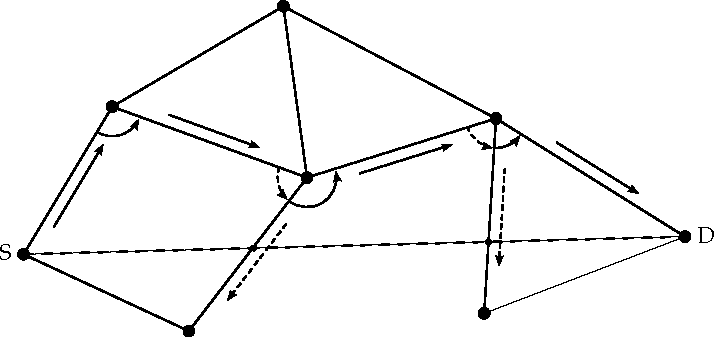
\includegraphics{recuperacion_gpsr}
\decoRule
\caption[Modo de recuperación de GPSR]{Modo de recuperación de
GPSR\protect\footnotemark.}
\label{fig:recuperacion_gpsr}
\end{figure}

\footnotetext{Adaptación del esquema presentado por Mauve\cite{Mauve2001}.}

\subsubsection{Inundación direccional restringida}
%-----------------------------------
%   INUNDACIÓN DIRECCIONAL RESTRINGIDA
%-----------------------------------
\label{subsubsec:inundacion_direccional_restringida}

El protoclo DREAM, discutido en la sección
\ref{subsec:servicios_de_localizacion}, usa esta técnica de retransmisión de
paquetes. En la figura \ref{fig:dream_region_esperada} se muestra el nodo S,
que quiere enviar un paquete al nodo D. El nodo S transmite el paquete a todos
sus vecinos que se encuentran en la dirección del nodo D. Para determinar esta
dirección, se calcula la región donde es probable que se encuentre el nodo D,
llamada \textit{región esperada}. Debido a que nada impide que el nodo D se
pueda mover en cualquier dirección, la región esperada es un círculo de radio
$v_{max}(t_1-t_0)$, donde $t_0$ es el tiempo en el que se registró la última
ubicación del nodo D, $t_1$ es el tiempo en el que se calcula la región
esperada, y $v_{max}$ es la velocidad máxima a la que se puede mover el nodo D.
El centro de este círculo es la ubicación del nodo D en el tiempo $t_0$.

\begin{figure}[th]
\centering
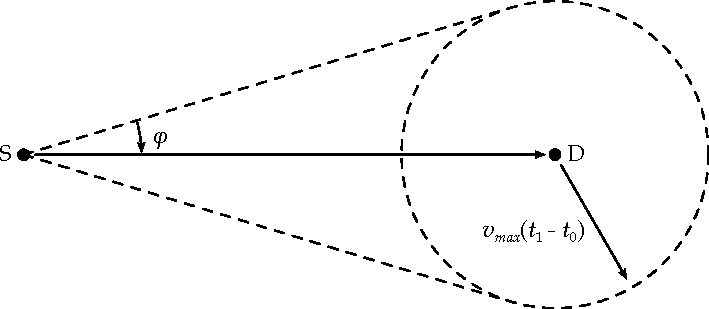
\includegraphics{dream_region_esperada}
\decoRule
\caption[Región esperada en el protocolo DREAM]{Región esperada en el protocolo
DREAM\protect\footnotemark.}
\label{fig:dream_region_esperada}
\end{figure}

\footnotetext{Adaptación del esquema presentado por Mauve\cite{Mauve2001}.}

Dada la región esperada, la dirección hacia el nodo D está delimitada por la
línea recta entre el nodo S y el nodo D y el ángulo $\varphi$. En otras
palabras, un nodo se encuentra en la dirección del nodo D si se encuentra
dentro del área delimitada por la región esperada y las dos líneas que empiezan
en el nodo S y son tangentes al círculo del perímetro de la región esperada. El
nodo S retransmite el paquete hacia sus vecinos que se encuentren en esa
dirección, y cada uno repite el proceso considerando su propia actualización de
la ubicación del nodo D. En caso de que no haya disponible un vecino que cumpla
con este criterio, se requiere un método de recuperación; sin embargo, este no
se especifica en el protocolo DREAM.

\subsubsection{Enrutamiento jerárquico}
%-----------------------------------
%   ENRUTAMIENTO JERÁRQUICO
%-----------------------------------
\label{subsubsec:enrutamiento_jerarquico}

Las redes de infraestructura fija pueden llegar a ser increíblemente complejas,
por lo que se organizan de manera jerárquica para lidiar con esta complejidad.
Por ejemplo, los enrutadores que forman el \textit{backbone} de la Internet se
organiza en \textit{Autonomous Systems} (ASs), o sistemas autónomos. El
enrutamiento de paquetes dentro del mismo AS se rige por un \textit{Interior
Gateway Protocol} (IGP)\footnote{Protocolo de puerta de enlace interior.}, como
el protocolo \textit{Open Shortest Path First} (OSPF)\footnote{Abrir el camino
más corto primero.} o \textit{Routing Information Protocol}
(RIP)\footnote{Protocolo de información de enrutamiento.}. Cuando un paquete
tiene que atravesar varios ASs, se utiliza un \textit{Interior Gateway Protocol}
(EGP)\footnote{Protocolo de puerta de enlace exterior.} al pasar de un AS a
otro; por ejemplo, \textit{Border Gateway Protocol} (BGP)\footnote{Protocolo
de puerta de enlace de frontera.}.
Esto facilita el enrutamiento a través de la Internet importantemente a pesar de
la enorme cantidad de dispositivos que la conforman. Por esta razón, es válido
preguntarse si el enrutamiento se puede beneficiar en las MANETs introduciendo
una estructura jerárquica.

En \cite{Blaevi2002}, Blaevi \textit{et al.} presentan el proyecto Terminode,
en el que se establece una jerarquía de dos niveles. El enrutamiento se hace
con un protocolo llamado \textit{Terminode Local Routing}
(TLR)\footnote{Enrutamiento local Terminode.} si el nodo de origen y el nodo de
destino están a pocos enlaces de distancia. TLR es un protocolo proactivo que
no usa las ubicaciones para seleccionar determinar las rutas. Cuando se trata
de distancias largas, se usa el protocolo \textit{Terminode Remote Routing}
(TRR)\footnote{Enrutamiento remoto Terminode.}, que usa el método voraz para
acercar el paquete al destinatario. Una vez que el paquete llega a una región
cercana al destinatario, TLR se encarga de que el paquete llegue al nodo
correspondiente. El funcionamiento del enrutamiento Terminode se muestra en la
figura \ref{fig:terminode}.

\begin{figure}[th]
\centering
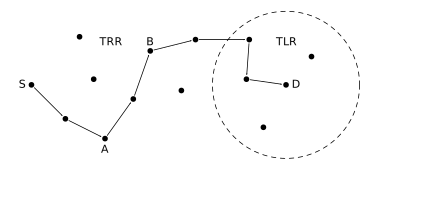
\includegraphics{terminode}
\decoRule
\caption[Enrutamiento Terminode]{Enrutamiento Terminode.}
\label{fig:terminode}
\end{figure}

Para prevenir que el protocolo TRR alcance un máximo local, el remitente incluye
una lista de ubicaciones por las que debe pasar el paquete. En la figura
\ref{fig:terminode}, se trata de los nodos A y B. Este método tiene cierta
similitud con la ruta de origen del protocolo DSR discutido en la sección
\ref{subsec:enrutamiento_reactivo}. Para conocer estas ubicaciones, el nodo
de origen solicita esta información a los nodos con los que tiene contacto
mediante TLR. Una vez que el nodo consigue esta información, debe verificar que
esta ruta de ubicaciones sigue vigente y si se puede optimizar.

\subsection{Protocolos de enrutamiento basados en la posición para VANETs}
%-----------------------------------
%   PROTOCOLOS DE ENRUTAMIENTO BASADOS EN LA POSICIÓN
%-----------------------------------
\label{subsec:protocolos_de_enrutamiento_basados_en_la_posicion_para_vanets}

Las características particulares de las VANETs introducen retos que no se
presentan en otros tipos de redes durante el proceso de enrutamiento. En esta
sección, se discuten algunos protocolos de enrutamiento especialmente diseñados
para lidiar con algunas de estas dificultades.

\subsubsection{GSR}
%-----------------------------------
%   GSR
%-----------------------------------
\label{subsubsec:gsr}

En \cite{Lochert2003}, Locher \textit{et al.} analizan las debilidades del
protocolo GPSR en un ambiente urbano, y proponen el protocolo
\textit{Geographic Source Routing} (GSR)\footnote{Enrutamiento de origen
geográfico.}. Este protocolo se apoya en un mapa de la ciudad para hacer el
enrutamiento basado en la posición.

Uno de los principales problemas del protocolo GPSR es que no considera la
existencia de obstáculos que deterioran la comunicación entre los nodos, como
los edificios en el ambiente de una VANET. Con el protocolo GSR, cuando un nodo
envía un paquete, usa el algoritmo de Dijkstra para calcular la ruta como una
secuencia de intersecciones de calles que el paquete debe atravesar para llegar
a su destino. Cuando un paquete viaja de una intersección a otra, se usa el
enfoque voraz para la retransmisión, ya que se asume que a lo largo de la calle
no existen obstáculos importante. Sin embargo, no incluye un método para
asegurar que a lo largo no se encuentre un máximo local.

GSR usa un servicio de localización simple llamado \textit{Reactive Location
Service} (RLS)\footnote{Servicio de localización reactivo.}. Cuando un nodo
necesita conocer la ubicación de otro, inunda la red con un mensaje de
solicitud. Si el nodo buscado recibe el mensaje, envía una respuesta con su
ubicación al nodo que hizo la solicitud. Este mecanismo incluye algunos
optimizaciones para evitar saturar toda la red con este tipo de solicitudes.

\subsubsection{SRPMT}
%-----------------------------------
%   SRPMT
%-----------------------------------
\label{subsubsec:srpmt}

El protocolo \textit{Street-centric Routing Protocol based on Microtopologies}
(SRPMT)\footnote{Protocolo de enrutamiento centrado en calles basado en
microtopologías.}, desarrollado por Zhang \textit{et al.} \cite{Zhang2016}
introduce el concepto de \textit{microtopología} (MT), que es un subconjunto de
toda la topología de la VANET. La MT comprende a los vehículos que se encuentran
a lo largo de una calle entre dos intersecciones consecutivas, y los enlaces
entre ellos, como se muestra en la figura \ref{fig:microtopologia}.

\begin{figure}[th]
\centering
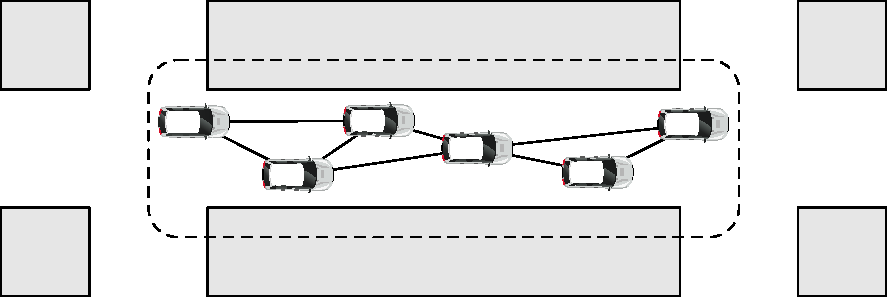
\includegraphics{microtopologia}
\decoRule
\caption[Microtopología]{Microtopología\protect\footnotemark.}
\label{fig:microtopologia}
\end{figure}

\footnotetext{Adaptación del esquema presentado por Zhang
\textit{et al.}\cite{Zhang2016}.}

Para llevar un paquete del nodo de origen al nodo de destino, la ruta puede
pasar por varias MTs. La estrategia de enrutamiento del protocolo SRPMT consiste
en dos pasos. El primero es determinar hacia qué MT se tiene que dirigir un
paquete una vez que llega al final de la MT que se encuentra atravesando. El
segundo paso es llevar el paquete del inicio de la MT hasta el final mediante
saltos por los nodos que la conforman. Cuando llega al último nodo de la MT,
este obtiene información de las MTs adyacentes y retransmite el paquete hacia
la que este nodo determine.

Este proceso se ilustra en la figura \ref{fig:ruta_microtopologias}, donde el
nodo S envía un paquete dirigido al nodo D. La microtopología $MT_{ij}$ comienza
en la intersección i y termina en la intersección j. Las flechas que se
encuentran dentro de la MT representan la dirección del avance del paquete a lo
largo de la MT. Las flechas que van de una MT a otra representan la selección
de la siguiente MT en la ruta.

\begin{figure}[th]
\centering
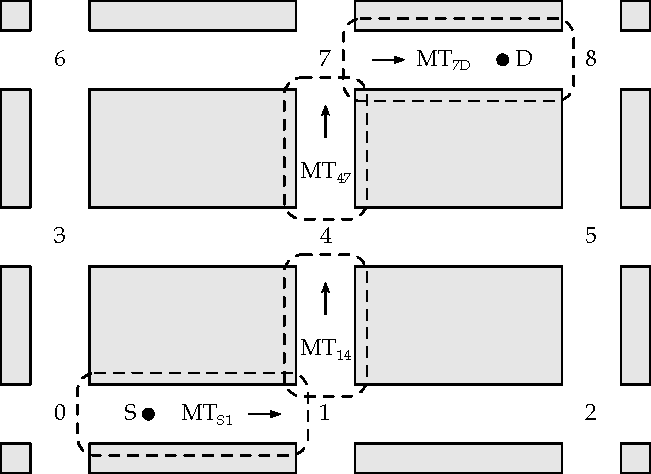
\includegraphics{ruta_microtopologias}
\decoRule
\caption[Ruta a lo largo de varias microtopologías]{Ruta a lo largo de
varias microtopologías\protect\footnotemark.}
\label{fig:ruta_microtopologias}
\end{figure}

\footnotetext{Adaptación del esquema presentado por Zhang
\textit{et al.}\cite{Zhang2016}.}

A pesar de que una MT puede modificarse constantemente según la movilidad de los
autos, la dirección hacia la que se tiene que mover el paquete es fija. Esto
significa que criterio para la retransmisión es que el paquete avance hacia el
extremo de la MT. Existen dos factores principales que afectan el desempeño de
una MT. El primero es el desempeño del enlace, que incluye la tasa de éxito de
transmisión de paquetes, y la demora en la entrega de paquetes. El otro factor
determinante es la estrategia de enrutamiento interna de la MT.

\subsubsection{MM-GPSR}
%-----------------------------------
%   MM-GPSR
%-----------------------------------
\label{subsubsec:mm_gpsr}

El protocolo GPSR, presentado en la sección \ref{subsubsec:retransmision_voraz},
selecciona como siguiente salto el nodo más cercano al destinatario. El
principal problema es que, mientras más cercano esté un nodo del destinatario,
más lejos se encuentra del nodo que debe hacer la retransmisión del paquete.
Por esto, existe la posibilidad de que el nodo seleccionado quede fuera del área
de transmisión antes de recibir la transmisión correctamente. Esta situación se
puede presentar más fácilmente en una VANET que en otros tipos de redes
\textit{ad hoc}, debido a que el movimiento relativo entre los vehículos es muy
rápido, y pueden cambiar de dirección abrúptamente y perder el enlace de
comunicación.

Es por esto que Yang \textit{et al.} proponen el protocolo
\textit{Maxduration-Minangle GPSR} (MM-GPSR)\footnote{Enrutamiento voraz y de
perímetro sin estado de másxima duración y ángulo mínimo.} \cite{Yang2018},
cuya principal característica es la modificación del criterio voraz de
selección del siguiente salto que se usa en GPSR. En la figura \ref{fig:mmgpsr}
se muestra la regla voraz del protocolo MM-GPSR, en el que el nodo S quiere
transmitir un paquete al nodo D. Primero, se determina el vecino más cercano al
nodo D, que es el nodo B en el ejemplo. Después, se obtiene la distancia
$d_{BD}$ entre los nodos B y D, y la distancia $d_{SB}$ entre los nodos S y B.
Posteriormente, se calcula $d_{max}$ con la ecuación \ref{eq:1}. Con estos
datos, se consideran dos círculos, el primero con centro en el nodo S y cuyo
radio es la distancia máxima de transmisión de este, y el segundo con centro en
el nodo D y con radio $d_{max}$. La región delimitada por la intersección de
ambos círculos se denomina $Q$. Cada nodo dentro de $Q$ se encuentra cerca del
nodo D, y está dentro del radio de comunicación del nodo S, por lo que es
apropiado para ser seleccionado para la retransmisión.

\begin{equation}
\label{eq:1}
d_{max} = d_{BD} + \lambda d_{SB}
\end{equation}

\begin{figure}[th]
\centering
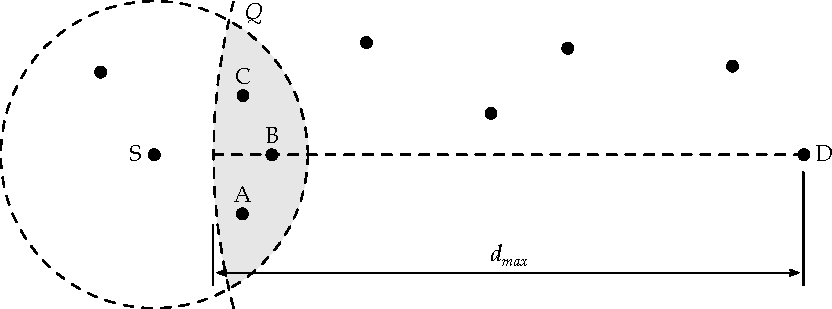
\includegraphics{mmgpsr}
\decoRule
\caption[Enrutamiento voraz en el protocolo MM-GPSR]{Enrutamiento voraz en el
protocolo MM-GPSR\protect\footnotemark.}
\label{fig:mmgpsr}
\end{figure}

\footnotetext{Adaptación del esquema presentado por Yang \textit{et
al.}\cite{Yang2018}.}

En la ecuación \ref{eq:1}, $\lambda$ puede variar desde 0 hasta 1. Si $\lambda$ se
acerca a 1, el área de $Q$ se hace más grande, y los vecinos más cercanos al nodo S
tienen oportunidad de ser seleccionados como siguiente salto, pero la cantidad
de saltos en la ruta incrementa. Si $\lambda$ se hacerca a 0, el área de $Q$ se
hace más pequeña, y los vecinos más lejanos al nodo S tienen más oportunidad
de ser seleccionados, por lo que la estabilidad del enlace puede empeorar
y la probabilidad de que se pierda el paquete aumenta.

Para seleccionar el siguiente salto, se considera la duración acumulada del
enlace de comunicación del nodo S con sus vecinos. Este dato se calcula con la
ecuación \ref{eq:2}, donde $T_{i-1}$ es la duración acumulada anterior del
enlace, $t_i$ es el tiempo de recepción de un mensaje \textit{hola}, y $t_{i-1}$
es el tiempo de recepción del mensaje \textit{hola} anterior. Las condiciones
iniciales son $T_1 = 0$ y $t_1$ es el tiempo en el que se recibe el primer
mensaje \textit{hola}. Al comparar el valor de $T_i$ para los nodos A, B y C,
el nodo con el máximo valor de $T_i$ es el que se selecciona como siguiente
salto, ya que su enlace con el nodo S es el que tiene el mejor historial de
estabilidad.

\begin{equation}
\label{eq:2}
T_i = T_{i-1} + t_i - t_{i-1}
\end{equation}

\subsubsection{VBRP}
%-----------------------------------
%   VBRP
%-----------------------------------
\label{subsubsec:vbpr}

Ji \textit{et al.} desarrollaron el protocolo \textit{Virtual Backbone-based
Routing Protocol} (VBRP)\footnote{Protocolo de enrutamiento basado en
\textit{backbone} virtual.} \cite{Ji2019}, en el que cada nodo puede ser de dos
tipos: normal o \textit{backbone}. Los nodos \textit{backbone} son las únicos
que partiipan en el enrutamiento, mientras los nodos normales pueden transmitir
y recibir paquetes a través de los nodos \textit{backbone}. La idea de dejar
fuera del enrutamiento a ciertos nodos es no saturar el canal de comunicación
para reducir las demoras por contenciones y prevenir las colisiones entre las
transmisiones. Para seleccionar los nodos \textit{backcone}, se define una
métrica llamada \textit{Stability Index} (SI), o índice de estabilidad. El SI
se obtiene a partir de dos parámetros, que son la estabilidad del enlace de
comunicación y la movilidad relativa entre los nodos. Los nodos con mayor SI se
seleccionan como nodos \textit{backbone}.

El funcionamiento general del protocolo VBPR se muestra en la figura
\ref{fig:vbpr}. El nodo S envía un paquete dirigido al nodo D, así que lo
transmite a un nodo \textit{backbone}, y este lo retransmite al siguiente nodo
\textit{backbone} que se encuentre adelante en el camino. En este protocolo
también se consideran dispositivos fijos llamadas \textit{Road Side Units}
(RSUs), o unidades laterales del camino, que toma las decisiones de
enrutamiento en las intersecciones.

\begin{figure}[th]
\centering
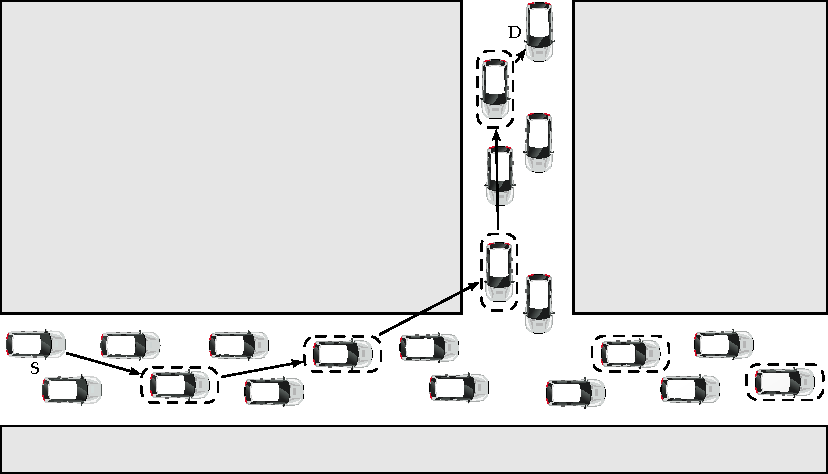
\includegraphics{vbpr}
\decoRule
\caption[Funcionamiento del protocolo VBRP]{Funcionamiento del protocolo VBRP\protect\footnotemark.}
\label{fig:vbpr}
\end{figure}

\footnotetext{Adaptación del esquema presentado por Ji
\textit{et al.}\cite{Ji2019}.}

%-----------------------------------
%   PROTOCOLO DE AUTOCONFIGURACIÓN DE DIRECCIONES PROPUESTO
%-----------------------------------
\chapter{Protocolo de autoconfiguración de direcciones propuesto}

\label{ch:autoconfiguracion_de_direcciones_propuesto}

Como se mencionó en el capítulo \ref{ch:autoconfiguracion_de_direcciones}, para
que los vehículos puedan comunicarse a través de la red, necesitan tener una
dirección IP. Al no contar con un servidor DHCP que se encargue de asignar una
dirección a cada vehículo, se requiere de un método que le permita a cada
vehículo obtener una dirección IP única de manera autónoma.

La razón por la que las direcciones IP tienen una estructura jerárquica, es que,
de este modo, los dispositivos que forman una red grande se pueden agrupar para
formar subredes, y esto facilita el enrutamiento. En las redes cableadas, la
jerarquización está determinada por la topología de la red. No obstante, en una
VANET, la topología cambia constantemente, por lo que se debe utilizar otro
método para agrupar a los vehículos y formar las subredes. En el presente
capítulo, se describe el protocolo de autoconfiguración de direcciones que se
diseñó para lograr este objetivo.

%-----------------------------------
%   FORMACIÓN DE LAS SUBREDES
%-----------------------------------
\section{Formación de las subredes}

\label{sec:formacion_de_subredes}

Una dirección IP se forma por dos partes, como se explica en la sección
\ref{subsec:direccionamiento_ipv6}: el prefijo, que identifica a la subred, y el
identificador asignado a la interfaz. Para que un vehículo pueda obtener una
dirección, lo primero que necesita conocer es la subred a la que se va a unir.
Esto nos lleva al problema de cómo agrupar a los vehículos para formar las
subredes.

Debido a las restricciones del canal de comunicación inalámbrica, como el
radio de transmisión, los vehículos se agrupan geográficamente. Es decir, una
subred se debe formar por el subconjunto de vehículos que se encuentran dentro
de cierta región geográfica. Si un vehículo es capaz de conocer su ubicación,
puede determinar en qué región se encuentra, y, por lo tanto, cuál es la red a
la que debe unirse. Por este motivo, se requiere que todos los vehículos
cuenten con algún dispositivo que les permita obtener su ubicación geográfica.

Después de definir la manera en la que se van a agrupar los vehículos para
formar las subredes, se debe especificar cómo se determinarán los límites de
cada región, y cómo asignar un código con el que se pueda generar el prefijo de
la subred para cada una. Para lograr esto, se recurrió al sistema de
codificación Geohash, que se describe en la siguiente sección.

%-----------------------------------
%   CODIFICACIÓN GEOHASH
%-----------------------------------
\subsection{Codificación Geohash}

\label{subsec:codificacion_geohash}

En el sistema de codificación Geohash, se representa una ubicación o una
región geográfica con una cadena corta de letras y números. La longitud del
codigo determina la precisión de la ubicación. Además, esta codificación permite
saber si dos ubicaciones son cercanas analizando la longitud del prefijo común
entre sus códigos \cite{wiki:Geohash}.

Un código Geohash es una cadena binaria, que se convierte en una secuencia de
símbolos de la codificación base 32, que se muestra en la tabla
\ref{tab:base32}.

\begin{table}[th]
\centering
\caption{Codificación base 32.}
\label{tab:base32}
\begin{tabular}{c c}
\toprule
\tabhead{Binario} & \tabhead{Base 32} \\
\midrule
00000 & 0 \\
00001 & 1 \\
00010 & 2 \\
00011 & 3 \\
00100 & 4 \\
00101 & 5 \\
00110 & 6 \\
00111 & 7 \\
01000 & 8 \\
01001 & 9 \\
01010 & b \\
01011 & c \\
01100 & d \\
01101 & e \\
01110 & f \\
01111 & g \\
\bottomrule
\end{tabular}
\quad
\begin{tabular}{c c}
\toprule
\tabhead{Binario} & \tabhead{Base 32} \\
\midrule
10000 & h \\
10001 & j \\
10010 & k \\
10011 & m \\
10100 & n \\
10101 & p \\
10110 & q \\
10111 & r \\
11000 & s \\
11001 & t \\
11010 & u \\
11011 & v \\
11100 & w \\
11101 & x \\
11110 & y \\
11111 & z \\
\bottomrule
\end{tabular}
\end{table}

Para formar un código Geohash, se divide toda la superficie de la Tierra en 32
celdas (figura \ref{fig:geohash1}), y a cada una se le asigna un símbolo. Se
elige la región que contiene la ubicación de interés y se agrega el símbolo
correspondiente al código. La región seleccionada se divide en 32 celdas (figura
\ref{fig:geohash2}), y nuevamente se selecciona la que contiene la ubicación, y
su símbolo se agrega al código. Este proceso se repite hasta obtener la
precisión necesaria. Se puede notar que, mientras más largo sea el prefijo
común entre dos códigos, más cercanas entre sí son las ubicaciones que
representan. En el apédice \ref{app:b} se explica con más detalle cómo
codificar una ubicación para obtener un código Geohash.

\begin{figure}[th!]
\centering
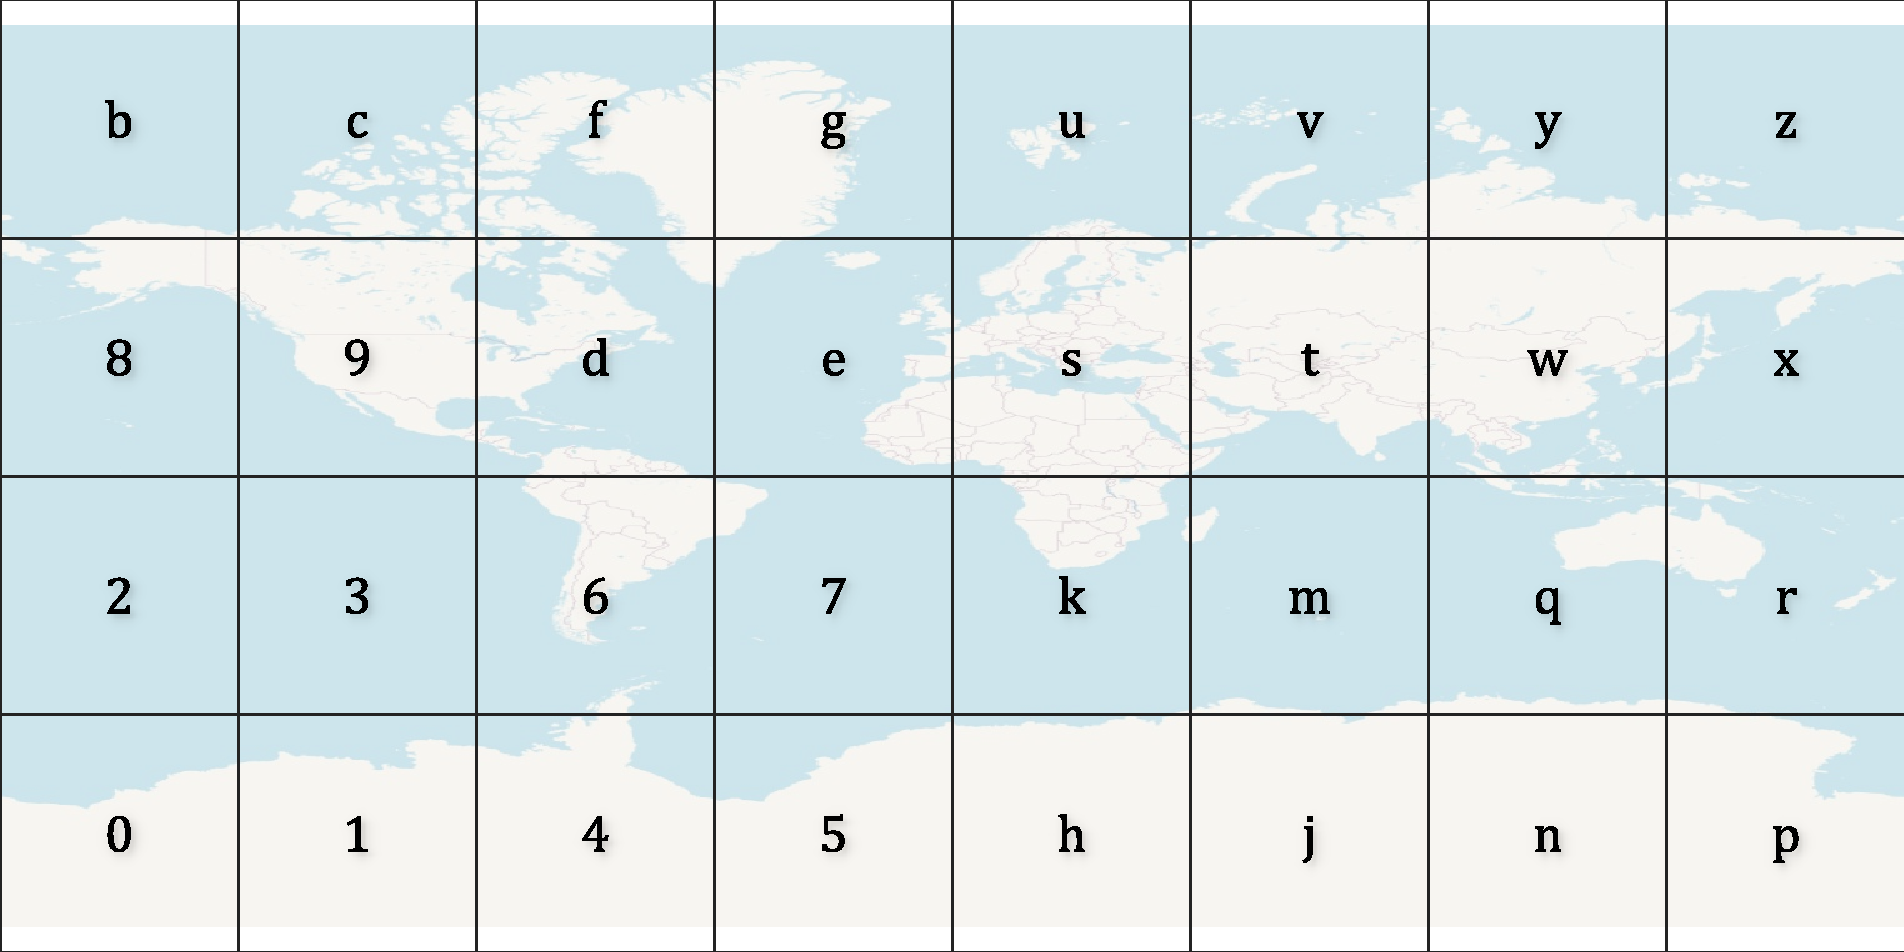
\includegraphics[width=0.85\textwidth]{geohash1} 
\decoRule
\caption[Códio Geohash de longitud 1]{Códio Geohash de longitud 1.}
\label{fig:geohash1}
\end{figure}

\begin{figure}[th!]
\centering
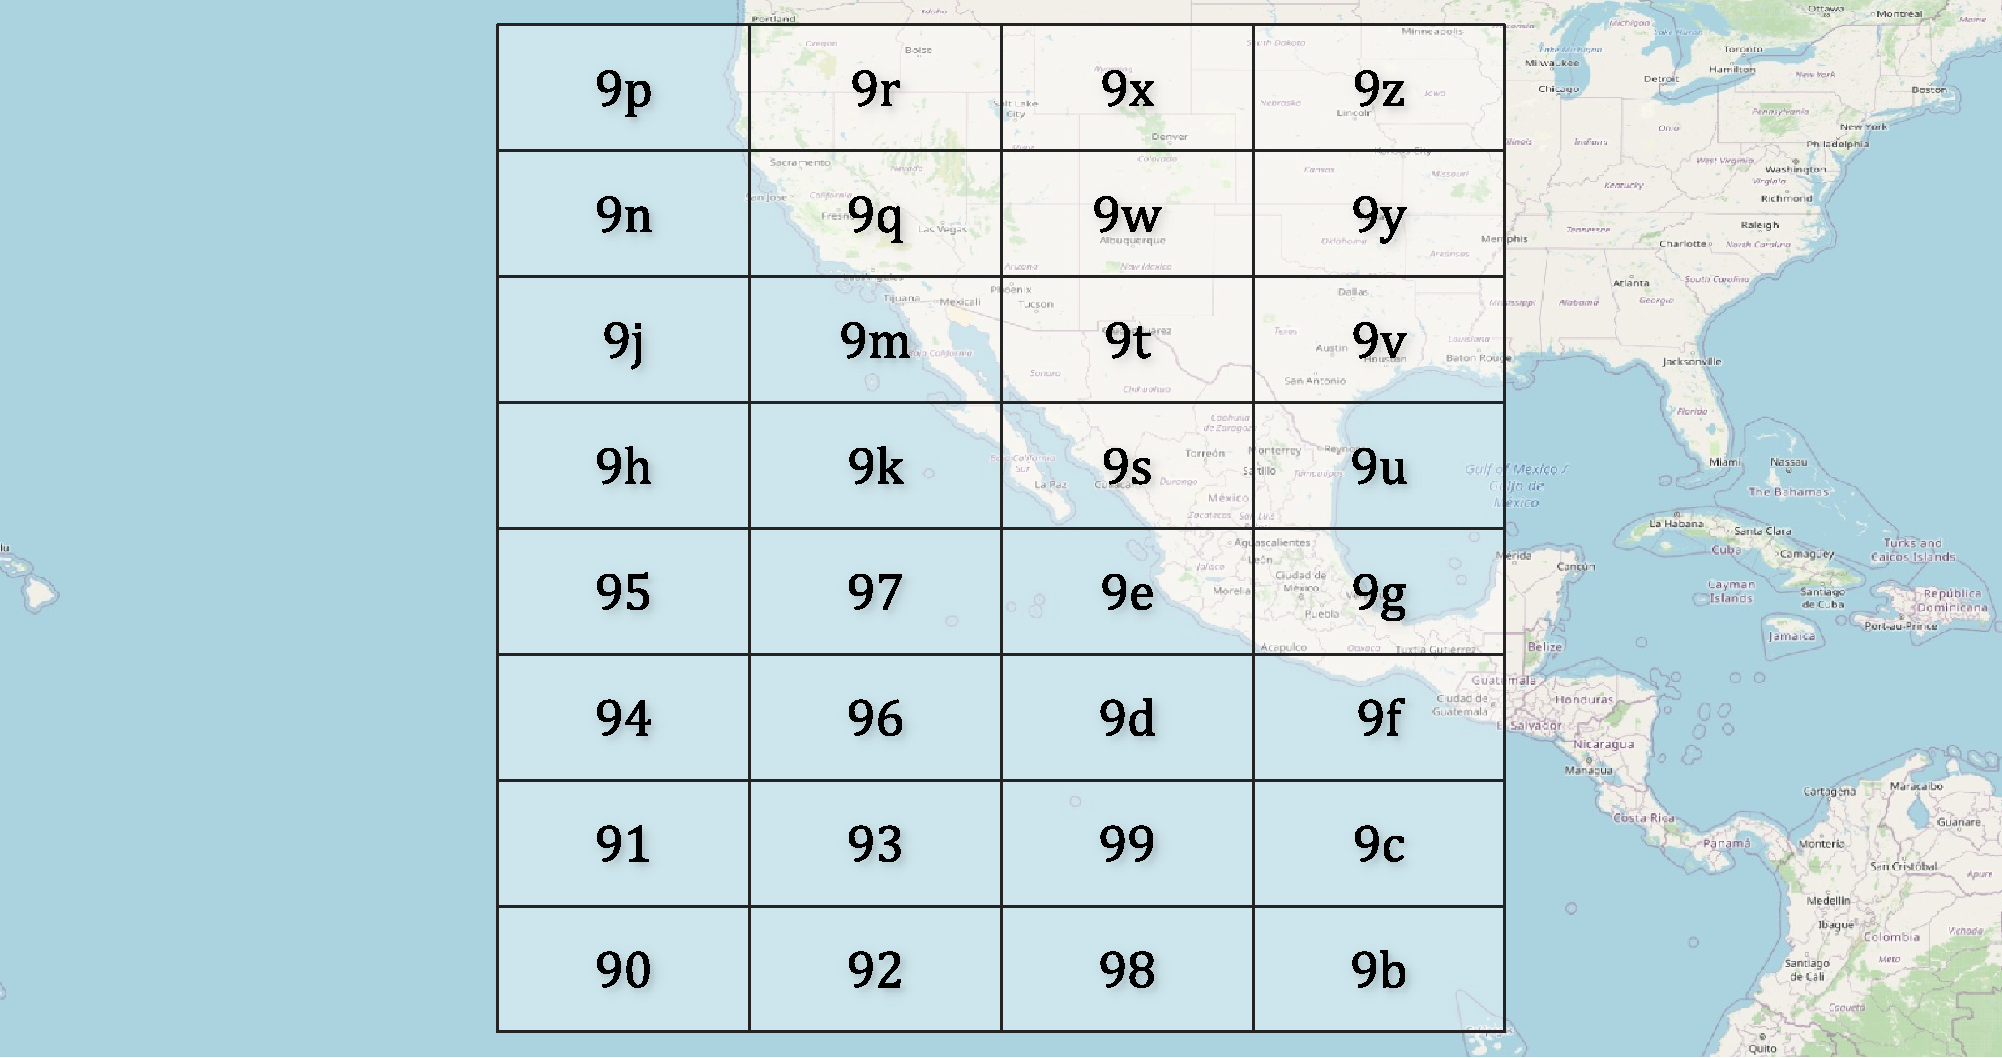
\includegraphics[width=0.85\textwidth]{geohash2}
\decoRule
\caption[Códio Geohash de longitud 2]{Códio Geohash de longitud 2.}
\label{fig:geohash2}
\end{figure}

Un mismo código se puede interpretar con una región o como una ubicación, en
cuyo caso, generalmente, se considera el centro de la región. En la tabla
\ref{tab:tamaño_celdas_geohash} se muestra el tamaño aproximado de las celdas
que se obtienen de acuerdo a la longitud del código. Se debe considerar que el
tamaño de las celdas es más pequeño a medida de que se alejan del ecuador
\cite{GeohashBolivia}.

\begin{table}[th]
\caption{Tamaño de las celdas para diferentes longitudes de código
\cite{GeohashBolivia}.}
\label{tab:tamaño_celdas_geohash}
\centering
\begin{tabular}{c c r r}
\toprule
\tabhead{Longitud del código} & & \tabhead{Ancho} & \tabhead{Alto}\\
\midrule
1 & $\leq$ & 5,000 km & 5,000 km\\
2 & $\leq$ & 1,250 km & 625 km\\
3 & $\leq$ & 156 km & 156 km\\
4 & $\leq$ & 39.1 km & 19.5 km\\
5 & $\leq$ & 4.89 km & 4.89 km\\
6 & $\leq$ & 1.22 km & 0.61 km\\
7 & $\leq$ & 153 m & 153 m\\
8 & $\leq$ & 38.2 m & 19.1 m\\
9 & $\leq$ & 4.77 m & 4.77 m\\
10 & $\leq$ & 1.19 m & 0.596 m\\
11 & $\leq$ & 149 mm & 149 mm\\
12 & $\leq$ & 37.2 mm & 18.6 mm\\
\bottomrule\\
\end{tabular}
\end{table}

A partir de aquí, se llamará código \textbf{Geohash-\textit{n}} a un código
Geohash de longitud \textit{n}. También, se entenderá como \textbf{región
Geohash} o \textbf{ubicación Geohash} a una región o ubicación, respectivamente,
representadas por un código Geohash.

% La división de las regiones se hace con base en la división que se deriva de
% este sistema de codificación. La longitud de códigos que se usa es 6, por lo que
% las regiones resultantes miden aproximadamente 1.22 km en longitud y 0.61
% km en latitud, según la tabla \ref{tab:tamaño_celdas_geohash}. Este tipo de
% códigos se pueden traducir de manera directa a cadenas de bits, por lo que se
% peden incorporar fácilmente a las direcciones IP. Cada símbolo del código se
% convierte en una secuencia de 5 bits, así que la longitud total del código es de
% 30 bits. Cuando un vehículo necesita saber en qué región se encuentra, calcula
% el código Geohash de su ubicación con una precisión de 6 símbolos, con lo que
% genera el identificador de subred para su dirección \textit{unicast} y el
% identificador de grupo para la dirección \textit{multicast}.

%-----------------------------------
%   SUBREDES GEOHASH
%-----------------------------------
\subsection{Subredes Geohash}

\label{subsec:subredes_geohash}

La codificación Geohash nos permite delimitar regiones y asociar un código a
cada una, por lo que sirve para resolver el problema planteado al final de la
sección \ref{sec:formacion_de_subredes}. Por esta razón, denominamos como
\textbf{subred Geohash} a una subred formada por los vehículos que se encuentran
dentro de una región Geohash. Ahora, se debe definir de qué tamaño deben ser
estas regiones.

Si las regiones fueran muy grandes, habría muy pocas subredes con muchos
vehículos cada una, por lo que no se aprovecharía la jerarquización de
direcciones que ofrece el protocolo IPv6, y esto complicaría el enrutamiento.
En la figura \ref{fig:region_geohash5} se puede notar que las regiones
Geohash-5 abarcan un área muy grande, por lo que se presentaría esta situación
si se eligiera este tamaño.

Por otra parte, si las regiones fueran muy pequeñas, habría muchas subredes con
muy pocos vehículos. En la figura \ref{fig:region_geohash7} podemos ver que las
regiones Geohash-7 son tan pequeñas, que algunas apenas abarcan un pequeño
segmento de alguna calle. Si se eligiera este tamaño, en algunos casos
podría llegar a haber regiones sin ningún vehículo. Además, algunos pares de
celdas adyacentes no cuentan con algún segmento de calle que las conecte, por
lo que los vehículos no podrían pasar de una región a otra.

Según la tabla \ref{tab:tamaño_celdas_geohash}, las regiones Geohash-6 son de
1.22 km de ancho y 0.61 km de alto, aproximadamente. En la figura
\ref{fig:region_geohash6} se puede ver que estas regiones tienen un tamaño más
apropiado que los de las regiones consideradas anteriormente.
Además, todas las regiones tienen al menos un segmento de calle que
las conecte con las cuatro regiones adyacentes. Es por esto que se decidió que
cada subred Geohash abarcará una región Geohash-6.

\begin{figure}[th!]
\centering

\begin{subfigure}{\textwidth}
\centering
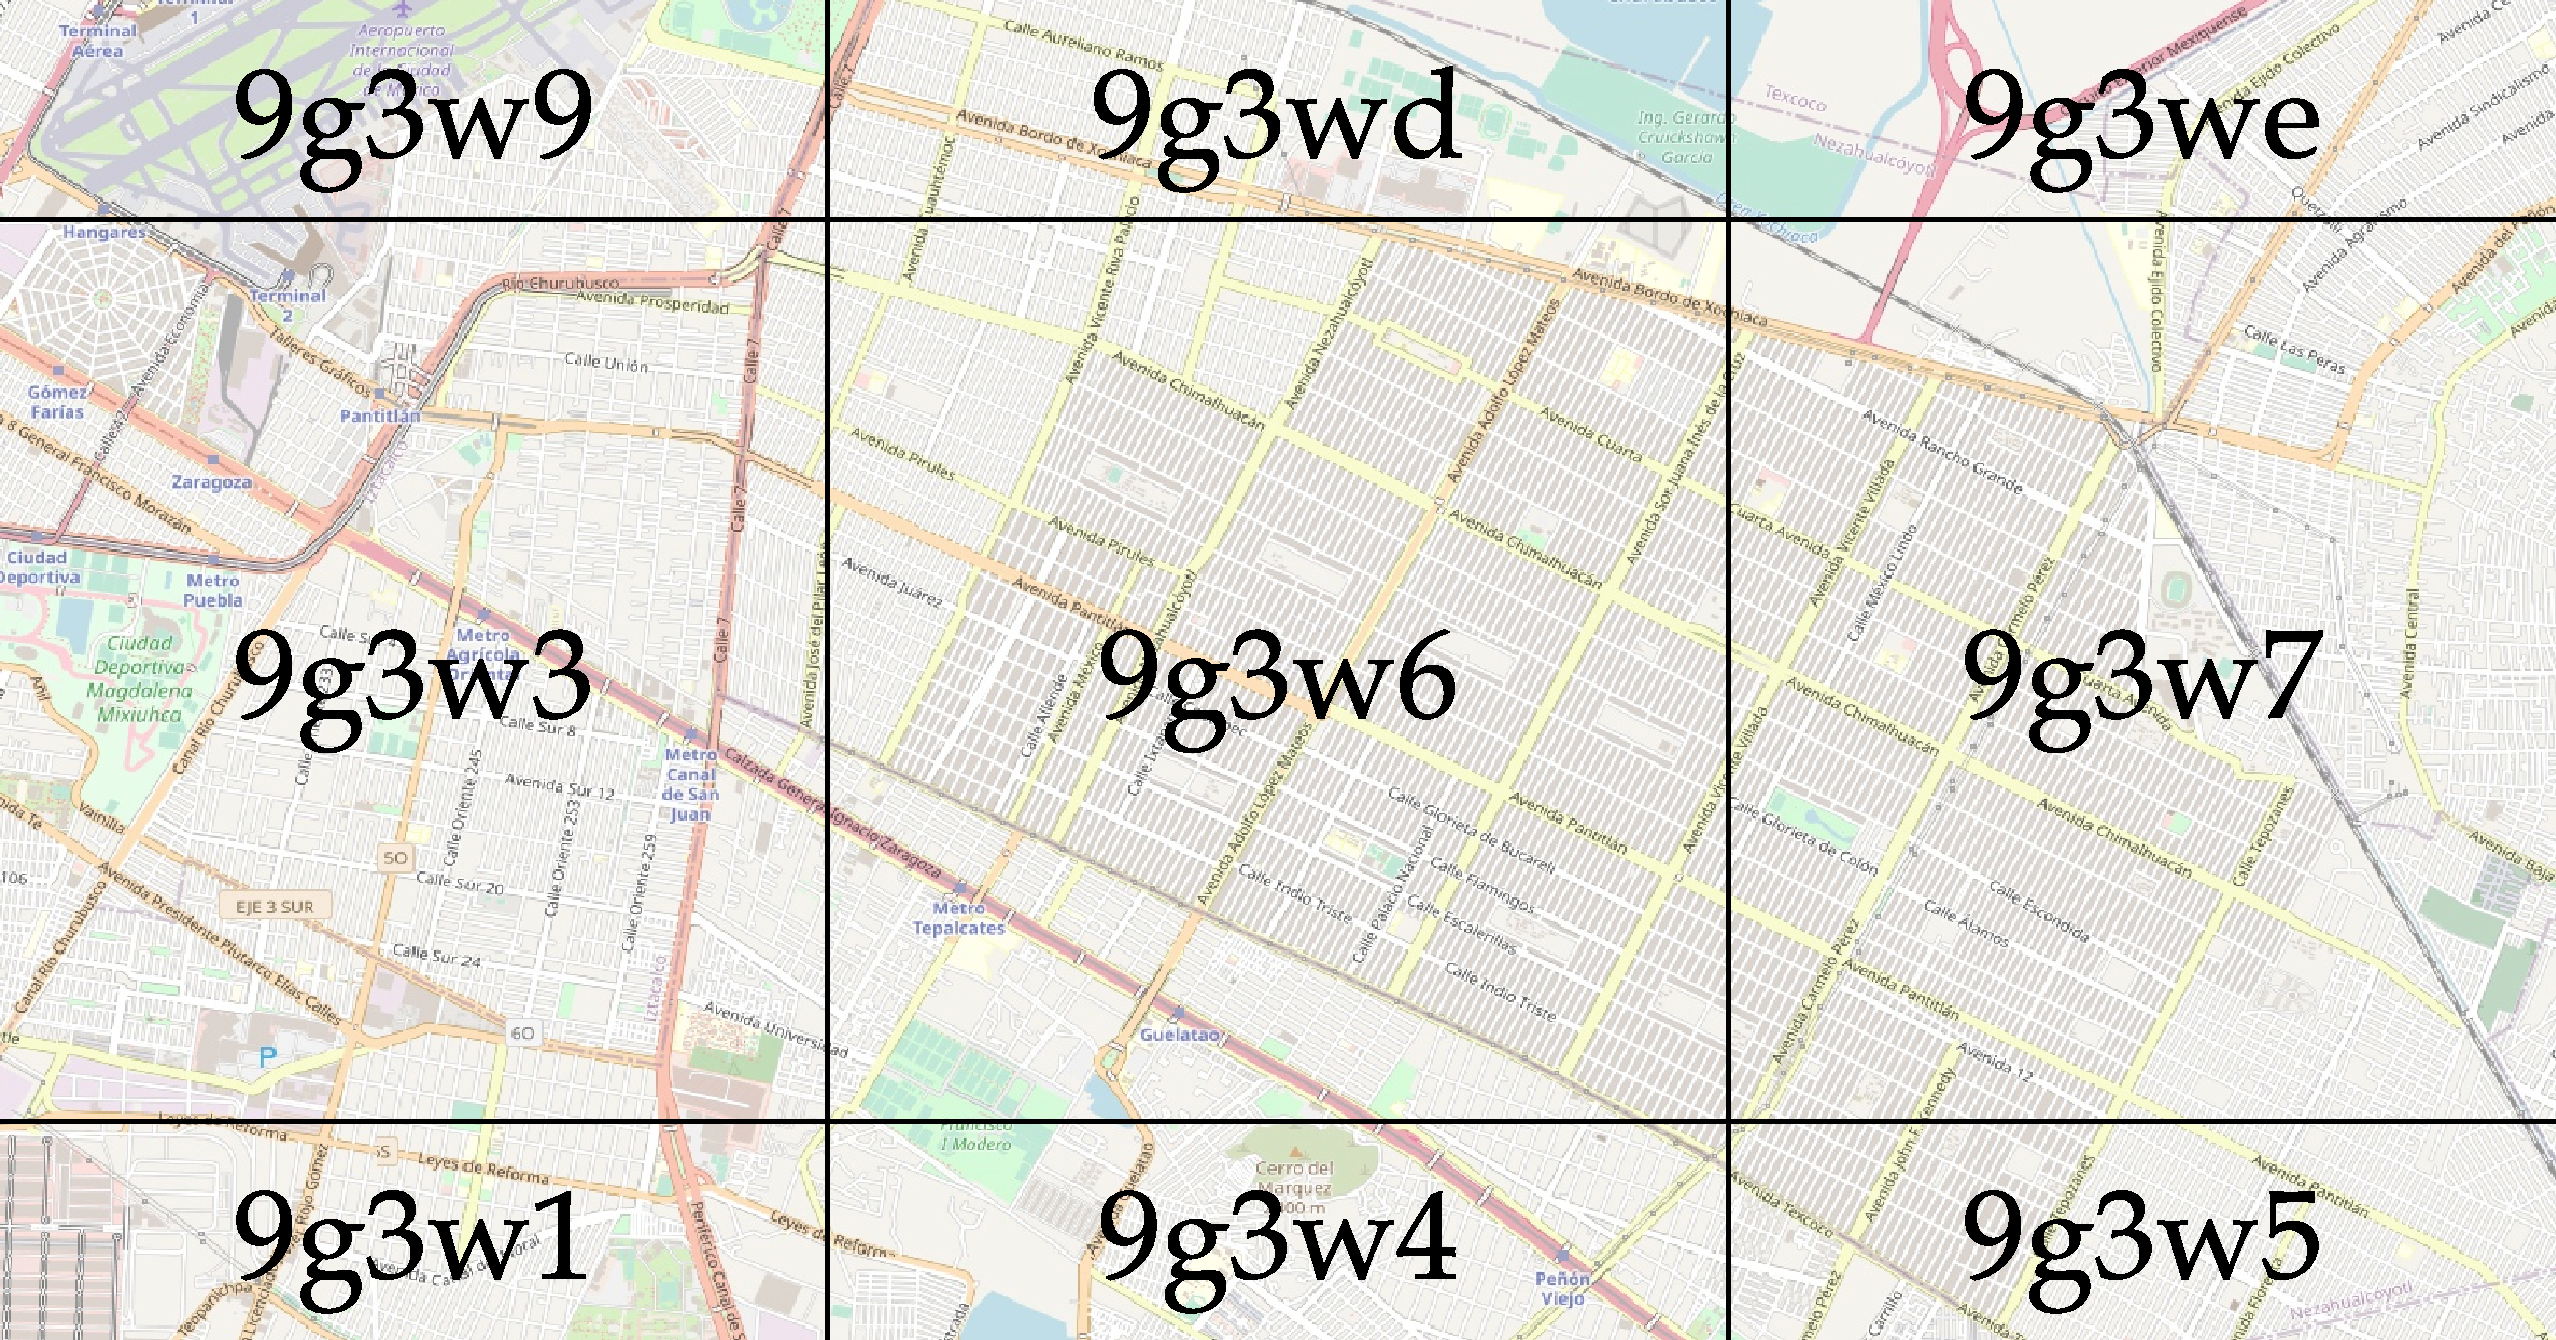
\includegraphics[height=4cm]{region_geohash5} 
\caption[Regiones Geohash-5]{Regiones Geohash-5.}
\label{fig:region_geohash5}
\end{subfigure}

\vspace{0.5cm}

\begin{subfigure}{\textwidth}
\centering
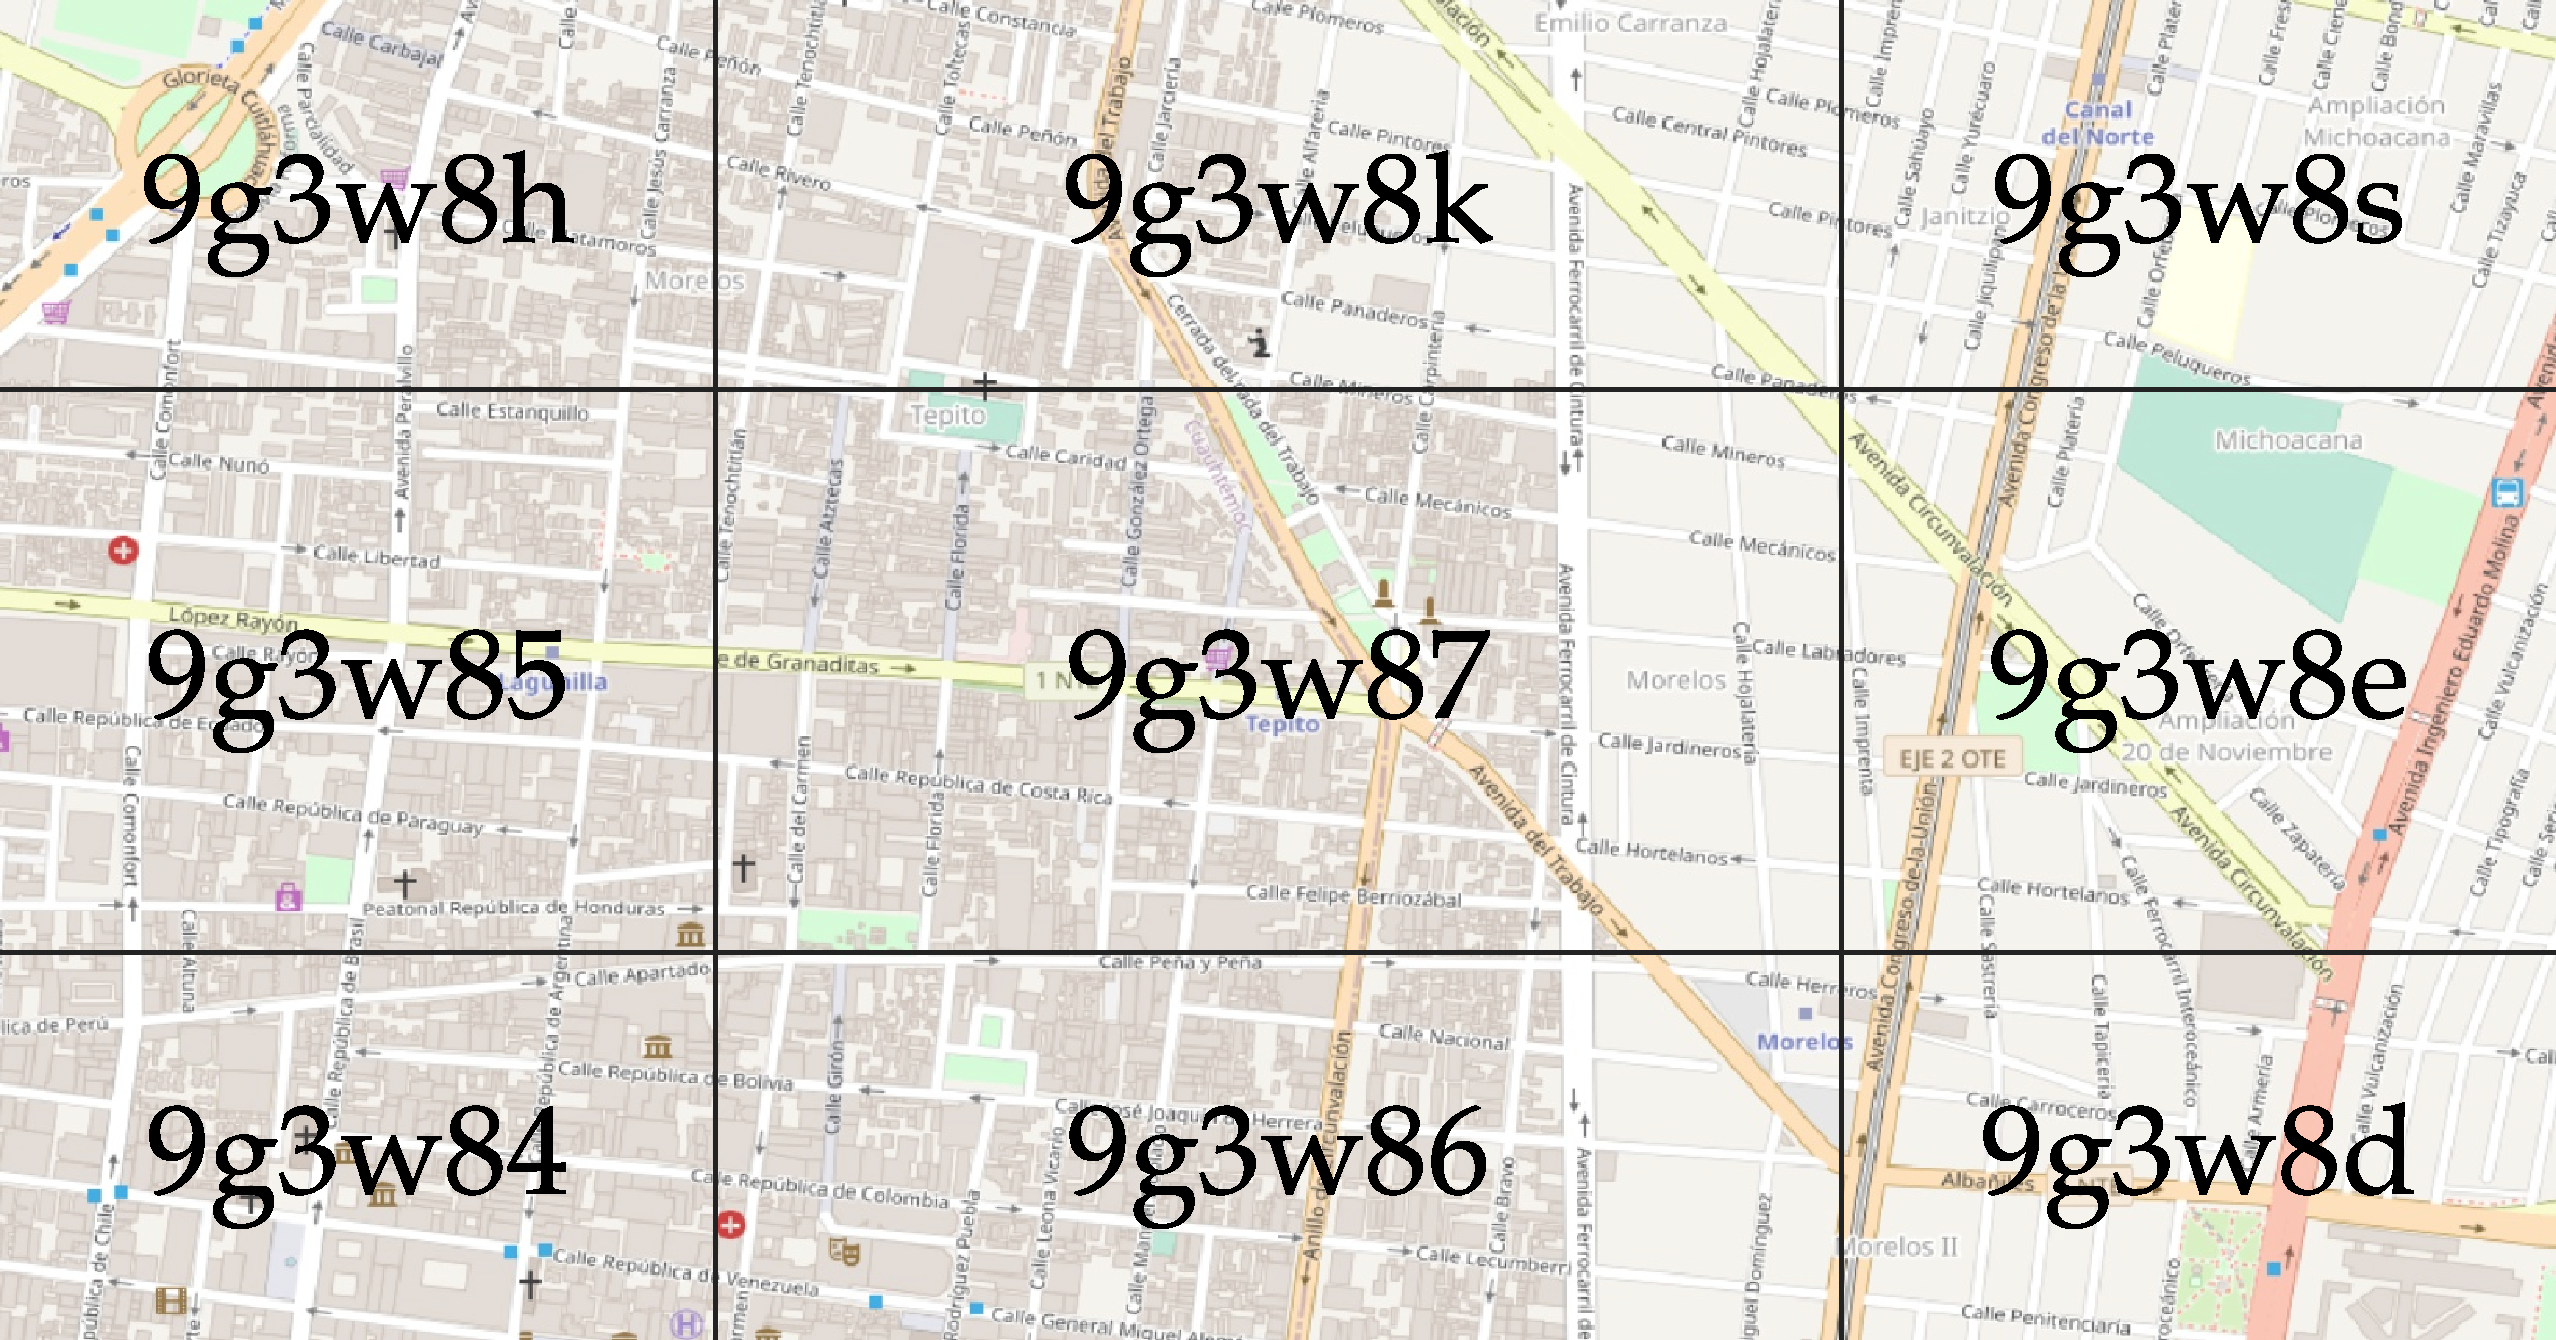
\includegraphics[height=4cm]{region_geohash6} 
\caption[Regiones Geohash-6]{Regiones Geohash-6.}
\label{fig:region_geohash6}
\end{subfigure}

\vspace{0.5cm}

\begin{subfigure}{\textwidth}
\centering
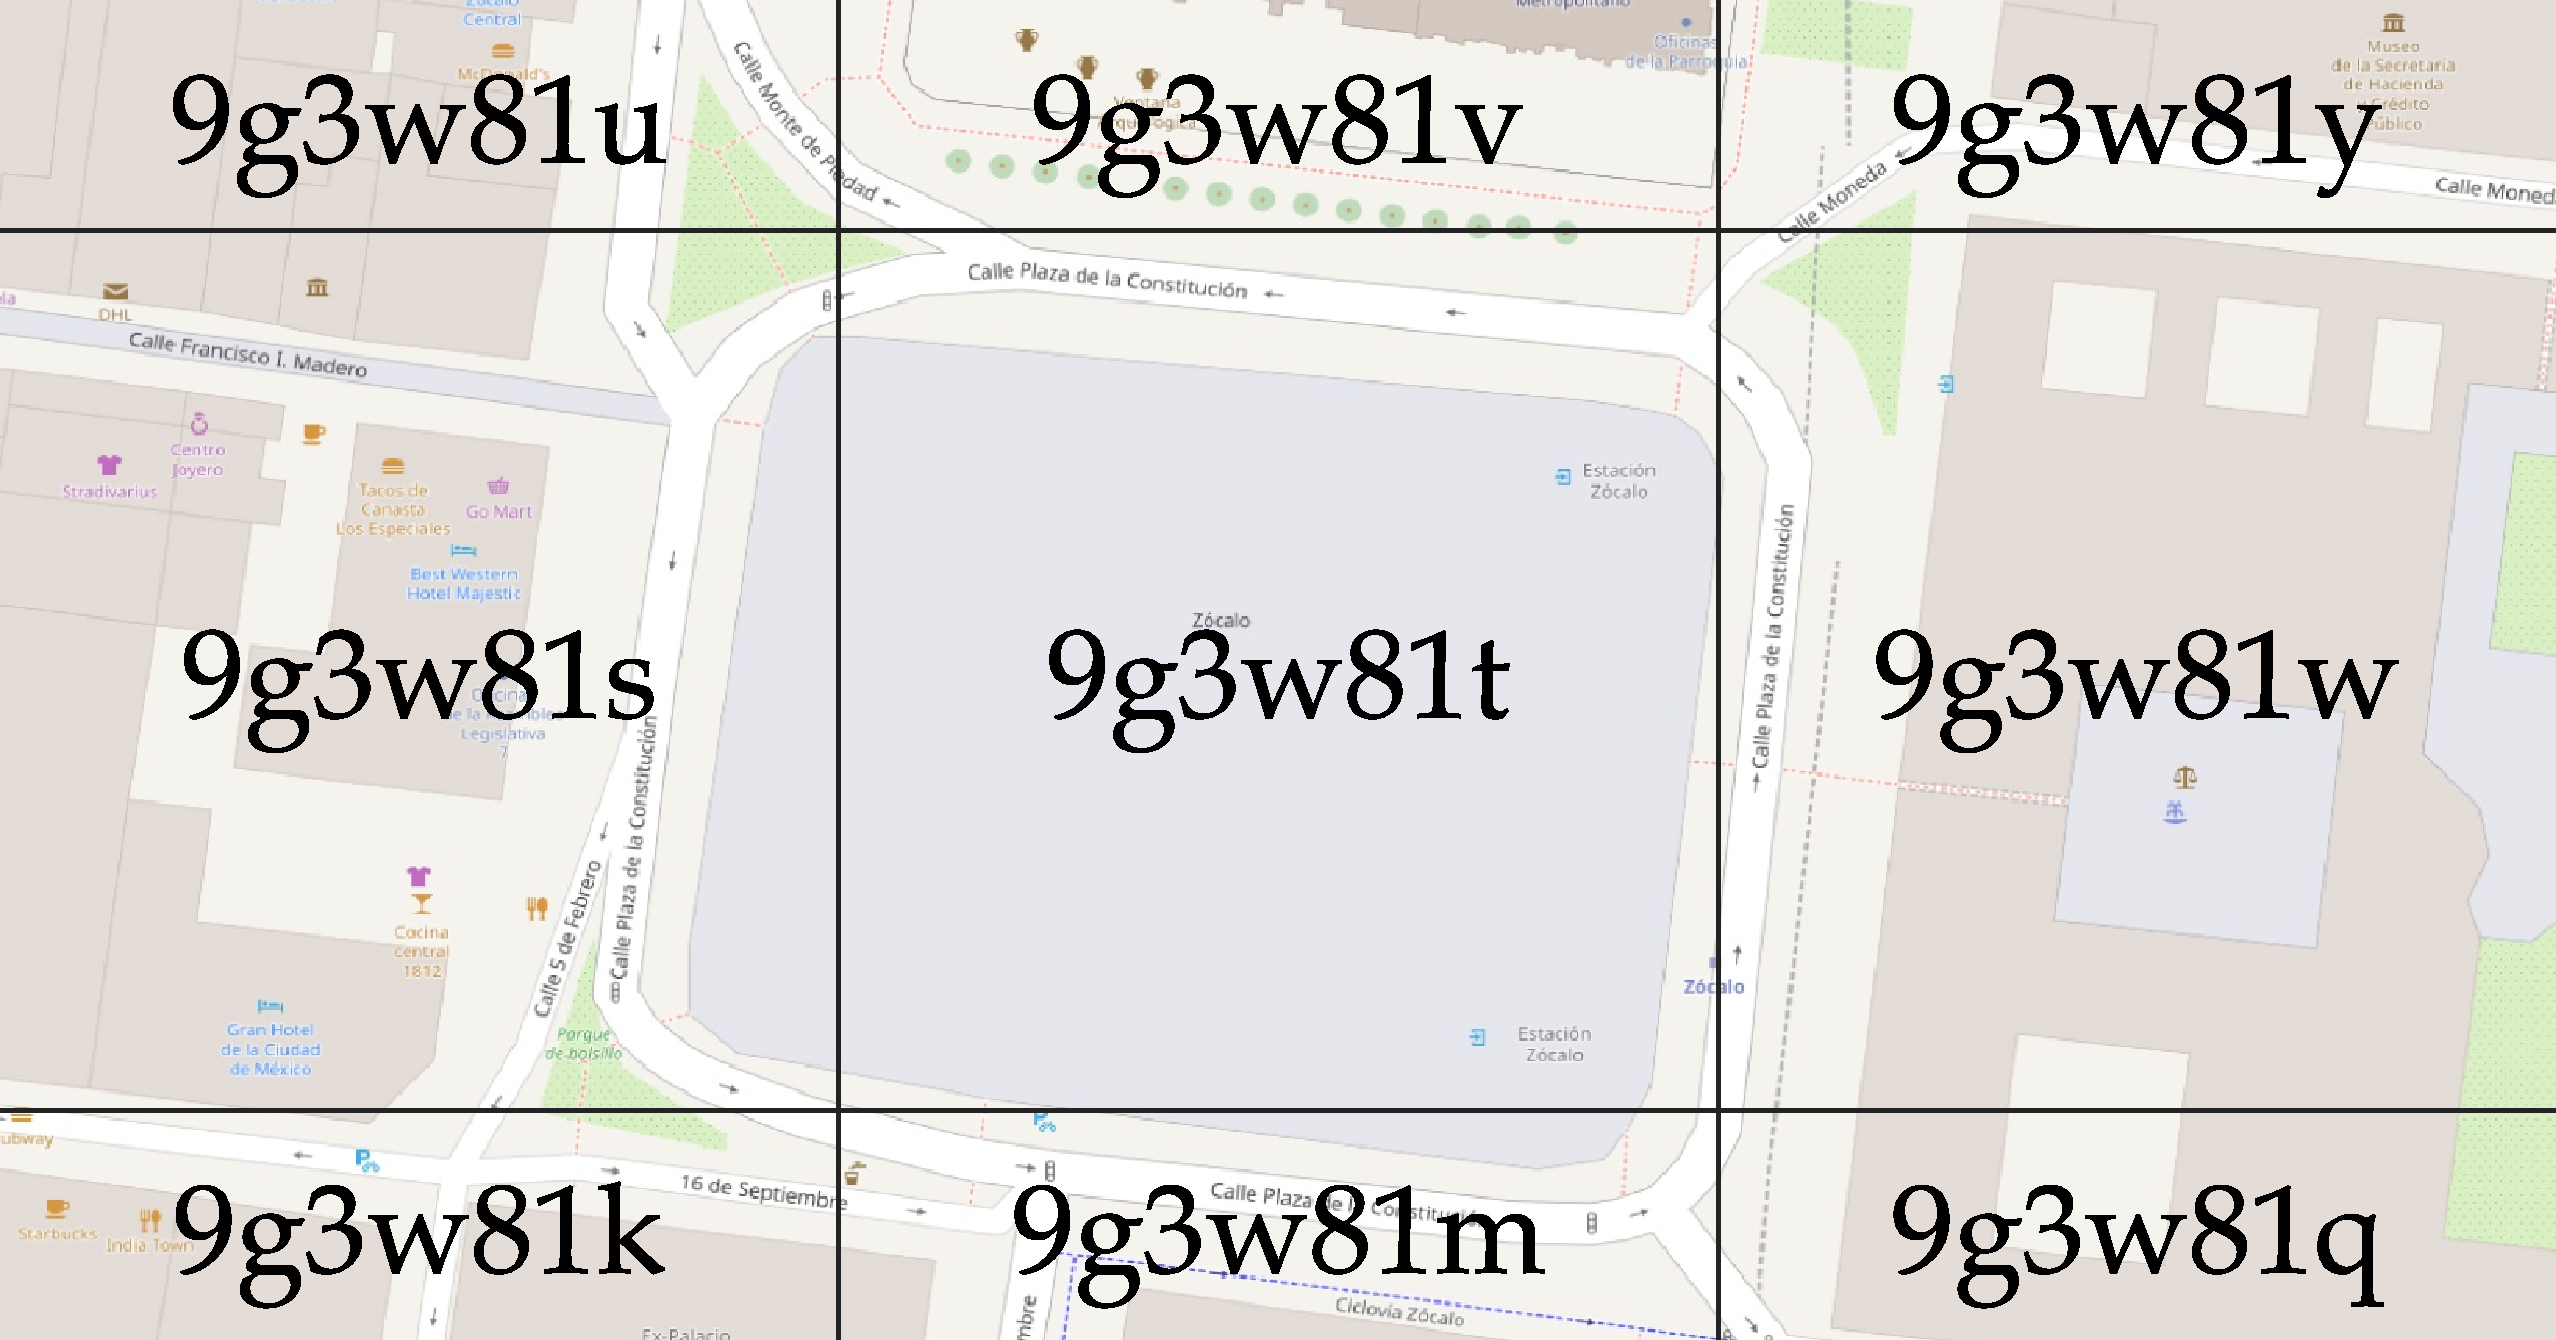
\includegraphics[height=4cm]{region_geohash7} 
\caption[Regiones Geohash-7]{Regiones Geohash-7.}
\label{fig:region_geohash7}
\end{subfigure}

\vspace{0.5cm}

\decoRule
\caption[Tamaños de regiones Geohash]{Tamaños de regiones Geohash.}
\label{fig:tamaños_geohash}

\end{figure}

Ya que se tiene definido el tamaño de cada región, en las siguientes
secciones se describe cómo se utilizan los códigos Geohash de cada una para
determinar formar las direcciones IP con las que los vehículos podrán
autoconfigurarse.

%-----------------------------------
%   FORMATO DE LAS DIRECCIONES IPV6 UNICAST
%-----------------------------------
\subsection{Formato de las direcciones IPv6 \textit{unicast}}

\label{subsec:formato_direcciones_ipv6_unicast}

Para que un vehículo pueda compartir paquetes con otro, ambos necesitan tener
una dirección IP \textit{unicast}. Este tipo de direcciones identifican de
manera única a un dispositivo dentro de una red. El protocolo IPv6 define
diferentes tipos de direcciones \textit{unicast}, que se describen a
continuación \cite{CiscoIpv62011}:

\keyword{Dirección global agregable} -- Estas direcciones tienen un prefijo de
enrutamiento global de 48 bits que comienza con \code{2000::/3}. En seguida,
tiene un identifiador de subred de  16 bits, y al final el identificador del
nodo de 64 bits. Su asignación depende de la Autoridad de Asignación de Números
de Internet (IANA) y los proveedores de servicio de Internet (ISPs).

\keyword{Dirección local de enlace} --  Se pueden configurar automáticamente con
el prefijo \code{FE80::/10} y el identificador de la interfaz con el formato
EUI-64 (\ref{app:a}). Se usa para el protocolo de descubrimiento de vecinos y
el proceso de autoconfiguración sin estado. Los paquetes destinados a este tipo de
dirección no son enrutados.

\keyword{Dirección compatible con IPv4} -- Son direcciones que comienzan con el
prefijo \code{::/96} seguido de una dirección IPv4 de 32 bits. Se asignan a
nodos que sportan tanto IPv4 como IPv6.

\keyword{Dirección local única} -- Inician con el prefijo \code{FC00::/7}. Son
direcciones únicas globalmente, y son destinadas únicamente para comunicación
local; es decir, no se enrutan hacia Internet. Su asignación no depende del ISP
o de alguna otra entidad reguladora.

Debido a que no hay restricciones para la asignación de direcciones locales
únicas, este es el tipo de dirección \textit{unicast} que se usarán para
identificar a los vehículos. La figura \ref{fig:formato_direccion_unicast}
muestra el formato de una dirección local única \cite{CiscoIpv62011}.

\begin{figure}[th!]
\centering
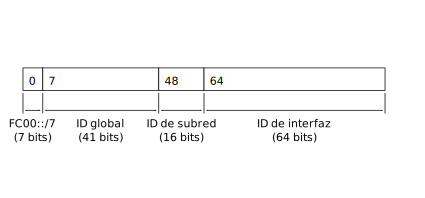
\includegraphics{formato_direccion_unicast}
\decoRule
\caption[Formato de una dirección local única]{Formato de una dirección
local única.}
\label{fig:formato_direccion_unicast}
\end{figure}

El identificador de la subred contiene el código Geohash asociado a esta, por
lo que las direcciones \textit{unicast} se denominan \keyword{direcciones
\textit{unicast} Geohash}. El formato destas direcciones se muestra en la
figura \ref{fig:formato_direccion_unicast_geohash}, y se conforma de la
siguiente manera:

\begin{figure}[th!]
\centering
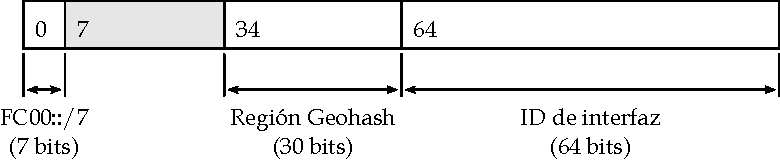
\includegraphics{formato_direccion_unicast_geohash}
\decoRule
\caption[Formato de una dirección \textit{unicast} Geohash]{Formato de una
dirección \textit{unicast} Geohash.}
\label{fig:formato_direccion_unicast_geohash}
\end{figure}

\keyword{Bits 0 - 6} -- Prefijo \code{FC00::/7}, que indica que se trata de
una dirección local única.

\keyword{Bits 7 - 33} -- No se usan; se fijan en 0.

\keyword{Bits 34 - 63} -- Código Geohash de la subred. Cuando un vehículo
conoce su ubicación, calcula el código Geohash, y los primeros 6 símbolos
corresponden al código de la subred. Este código se convierte a una cadena de
30 bits, de acuerdo con la tabla \ref{tab:base32}.

\keyword{Bits 64 - 127} -- Identificador de la interfaz en el formato
EUI-64.

%-----------------------------------
%   FORMATO DE DIRECCIONES IPV6 MULTICAST
%-----------------------------------
\subsection{Formato de direcciones IPv6 \textit{multicast}}

\label{subsec:formato_direcciones_ipv6_multicast}

Además de una dirección \textit{unicast}, cada vehículo necesita unirse a un
grupo \textit{multicast} para poder comunicarse con los demás de su misma
subred. En el protocolo IPv6, una dirección \textit{multicast} se forma por dos
partes: el prefijo \code{FF02::/16}, como se muestra en la figura
\ref{fig:formato_direccion_multicast}.

\begin{figure}[th!]
\centering
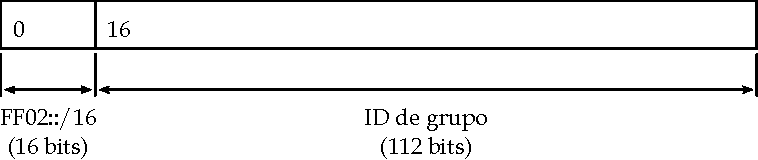
\includegraphics{formato_direccion_multicast}
\decoRule
\caption[Formato de una dirección \textit{multicast}]{Formato de una dirección
\textit{multicast}.}
\label{fig:formato_direccion_multicast}
\end{figure}

La dirección \textit{multicast} de cada subred también incluye el código
Geohash de esta, por lo que las direcciones \textit{mutlicast} se denominan
\keyword{direcciones \textit{multicast} Geohash}. El formato de estas
direcciones se muestra en la figura
\ref{fig:formato_direccion_multicast_geohash}, y se conforma de la siguiente
manera:

\keyword{Bits 0 - 15} -- Prefijo \code{FF02::/16}, que indica que se trata
de una dirección multicast.

\keyword{Bits 16 - 97} -- No se usan; se fijan en 0.

\keyword{Bits 98 - 127} -- Código Geohash de la subred. Cuando un vehículo
conoce su ubicación, calcula el código Geohash, y los primeros 6 símbolos
corresponden al código de la subred. Este código se convierte a una cadena de
30 bits, de acuerdo con la tabla \ref{tab:base32}.

\begin{figure}[th!]
\centering
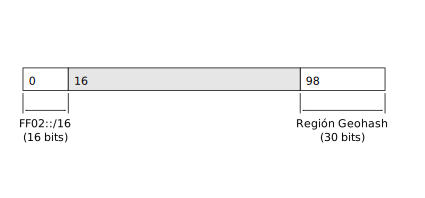
\includegraphics{formato_direccion_multicast_geohash}
\decoRule
\caption[Formato de la dirección \textit{multicast} para cada región]{Formato de
la dirección \textit{multicast} para cada región.}
\label{fig:formato_direccion_multicast_geohash}
\end{figure}

%-----------------------------------
%   CAMBIO DE SUBRED
%-----------------------------------
\section{Cambio de subred}

\label{sec:cambio_subred}

Cuando un vehículo enciende su interfaz de red, lo único que necesita para
autoconfigurarse es conocer su ubicación. Con este dato, podrá obtener su
dirección \textit{unicast} y su dirección \textit{multicast}, como se explicó
en la sección anterior. Sin embargo, se necesita definir cómo llevará a cabo la
autoconfiguración cuando se mueva de una región Geohash a otra.

Si un vehículo, al consultar su ubicación, detecta que se encuentra en una nueva
región Geohash, lo más simple sería eliminar de la configuración de su interfaz
las direcciones \textit{unicast} y \textit{multicast} de la subred anterior, y
configurar las direcciones para unirse a la nueva subred. Pero, de este modo,
las subredes estarían completamente aisladas una de otra, por lo que no se
podría hacer un enrutamiento a través de varias subredes.

En la figura \ref{fig:gateways}, se muestra la frontera entre las subredes
A y B. Durante el enrutamiento, un paquete necesita ser transmitido del vehículo
A$_1$ al vehículo B$_1$. Para esto, A$_1$ primero debe transmitirlo a A$_2$,
que se encuentra en su misma subred. Después, A$_2$ debe retransmitirlo a B$_2$,
a pesar de que pertenecen a redes distintas. Finalmente, B$_2$ lo retransmite
hacia B$_1$, que está en su misma subred. Los vehículos A$_2$ y B$_2$ se
denominan \textbf{\textit{gateways}}.

\begin{figure}[th]
\centering
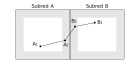
\includegraphics[width=8cm]{gateways}
\decoRule
\caption[Transmisión de paquetes de una subred a otra]{Transmisión de paquetes
de una subred a otra.}
\label{fig:gateways}
\end{figure}

Cuando un vehículo se encuentra dentro de los límites de una región Geohash, y
forma parte de la subred correspondiente a esa región, esta se denomina como
\textbf{subred primaria} del vehículo. La región resaltada de color gris en la
figura \ref{fig:gateways} se denota \textbf{región \textit{gateway}}.
Cuando un vehículo entra a la región \textit{gateway}, se auto-asigna las
direcciones \textit{unicast} y \textit{multicast} correspondientes a la subred
vecina. En el momento en que el vehículo forma parte también de la subred
vecina, esta se llama \textbf{subred secundaria} del vehículo. En la figura
\ref{fig:gateways}, el nodo A$_1$ tiene como subred primaria la subred A, y
no tiene subred secundaria, ya que no se encuentra dentro de la región gateway.
Para el nodo A$_2$, la subred primaria es la subred A, y la subred secundaria es
la B. Para el nodo B$_2$, la subred primaria es la B, y la secundaria es la A; y
para el nodo B$_1$, la subred primaria es la B, y no tiene subred secundaria.

Un \textit{gateway} deben tener la capacidad de recibir y transmitir paquetes
desde y hacia una subred vecina, por lo que debe ser parte de dos subredes a la
vez. Cualquier vehículo puede ser un \textit{gateway} si se encuentra cerca de
la frontera entre dos subredes. En el momento en que un vehículo se encuentre a
cierta distancia de la frontera, éste informa a los demás vehículos que se ha
convertido en un \textit{gateway}. Así, los demás podrán saber que a través de
él pueden transmitir paquetes hacia la subred vecina.

A continuación, se describe el procedimiento que lleva a cabo un vehículo cuando
se mueve de una subred a otra.

\begin{enumerate}
  \item El vehículo se encuentra dentro de una región Geohash, y su subred
  primaria es la correspondiente a la región. En la figura
  \ref{fig:cambio_subred1}, la subred primaria es la A.
  \item El vehículo entra a la región \textit{gateway} de la región Geohash
  donde se encuentra. En este momento, se une a la subred vecina como subred
  secundaria, y sigue siendo parte de la subred primaria. En la figura
  \ref{fig:cambio_subred2}, la subred secundaria es la B.
  \item El vehículo sale de la primera región Geohash y entra a la región
  \textit{gateway} de la nueva región. Aquí, la subred secundaria pasa a ser la
  región primaria --ya que ahora se encuentra físicamente en la nueva región--,
  y la región primaria pasa a ser la región secundaria. Sin embargo, todavía
  forma parte de ambas subredes. En la figura \ref{fig:cambio_subred3}, ahora la
  subred primaria es la B y la subred secundaria es la A.
  \item El vehículo sale de la región \textit{gateway} de la nueva región. A
  partir de aquí, el vehículo deja de pertenecer a la subred secundaria, ya que
  no es \textit{gateway} hacia ninguna otra subred. En la figura
  \ref{fig:cambio_subred4}, la subred primaria del vehículo es la B, y ya no
  tiene subred secundaria.
\end{enumerate}

\begin{figure}[th]
\centering

\begin{subfigure}{\textwidth}
\centering

\includegraphics[width=8cm]{cambio_subred1} 
\caption[Vehículo dentro de la primera región Geohash.]{Vehículo dentro de la
primera región Geohash.}
\label{fig:cambio_subred1}
\end{subfigure}

\vspace{0.5cm}

\begin{subfigure}{\textwidth}
\centering

\includegraphics[width=8cm]{cambio_subred2} 
\caption[El vehículo entra a la región \textit{gateway}.]{El vehículo entra a la
región \textit{gateway}.}
\label{fig:cambio_subred2}
\end{subfigure}

\vspace{0.5cm}

\begin{subfigure}{\textwidth}
\centering

\includegraphics[width=8cm]{cambio_subred3} 
\caption[El vehículo se mueve de una región Geohash a otra.]{El vehículo se
mueve de una región Geohash a otra.}
\label{fig:cambio_subred3}
\end{subfigure}

\vspace{0.5cm}

\begin{subfigure}{\textwidth}
\centering
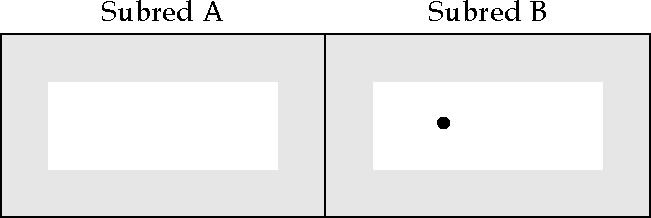
\includegraphics[width=8cm]{cambio_subred4} 
\caption[El vehículo sale de la región \textit{gateway}.]{El vehículo sale de
la región \textit{gateway}.}
\label{fig:cambio_subred4}
\end{subfigure}

\vspace{0.5cm}

\decoRule
\caption[Vehículo cambiando de una subred a otra]{Vehículo cambiando de una
subred a otra.}
\label{fig:cambio_subred}

\end{figure}


%-----------------------------------
%   PROTOCOLO DE ENRUTAMIENTO
%-----------------------------------
\chapter{Protocolo de enrutamiento}

\label{ch:protocolo_de_enrutamiento}

El protocolo de enrutamiento propuesto permite que dispositivos móviles puedan
comunicarse entre sí mediante el servicio de red proporcionado por la VANET.
Existen dos tipos de dispositivos que forman parte de la red. Los
\textit{hosts} son los dispositivos que ejecutan las aplicaicones que requieren
enviar información a otros. Los vehículos son los que se encargan de realizar
el enrutamiento de paquetes de un \textit{host} a otro.

Una vez que los vehículos tienen asignada una dirección IP, pueden comunicarse
entre sí a través de la red. Cuando un vehículo recibe un paquete, necesita
consultar su tabla de enrutamiento para saber hacia dónde lo debe retransmitir
para que llegue a su destino, como se menciona en la sección
\ref{sec:tablas_de_enrutamiento}. Sin embargo, se necesita un protocolo de
enrutamiento que se encargue de llenar la tabla.

Los vehículos tienen que compartir mensajes entre ellos con información que les
ayude a determinar hacia dónde tiene que enviar cada paquete de información. El
protocolo propuesto es basado en la posición, por lo que cada vehículo debe
compartir información, entre otras cosas, sobre su ubicación.

En este capítulo, se describe el funcionamiento del protocolo de enrutamiento
propuesto, es decir, cómo se determinan las rutas y los tipos de mensajes que
los vehículos se compartirán, además de cómo deben procesar estos mensajes para
llenar las tablas de enrutamiento.

%-----------------------------------
%   CRITERIOS GENERALES DE RETRANSMISIÓN DE PAQUETES
%-----------------------------------
\section{Criterios generales de retransmisión de paquetes}

\label{sec:criterios_generales_retransmision_paquetes}

Los protocolos basados en la posición, como se mencionó en la sección
\ref{sec:enrutamiento_basado_en_la_posicion}, consideran la ubicación de los
dispositivos para hacer decisiones sobre el enrutamiento. Por ejemplo, en el
protocolo GPSR, discutido en la sección \ref{subsubsec:retransmision_voraz},
cada nodo únicamente considera su ubicación, la del destinatario y las de los
vecinos, y selecciona el más cercano al destino. Sin embargo, en un ambiente
urbano es frecuente que existan obstáculos, principalmente edificios, que
bloqueen las transmisiones. Este tipo de transmisiones se conocen como
transmisiones sin \textbf{línea de visión}. La figura
\ref{fig:transmision_sin_linea_de_vision} muestra una transmisión en la que un
edificio se encuentra entre los vehículos A y B.

\begin{figure}[th]
\centering
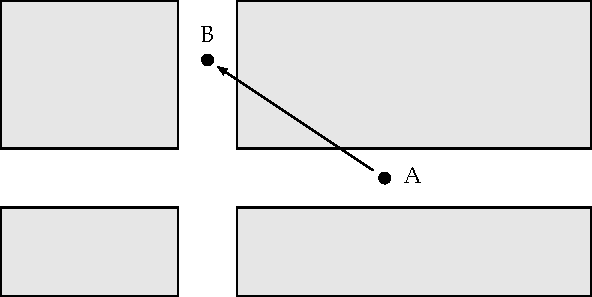
\includegraphics{transmision_sin_linea_de_vision}
\decoRule
\caption[Transmisión sin línea de visión]{Transmisión sin línea de visión.}
\label{fig:transmision_sin_linea_de_vision}
\end{figure}

Una transmisión sin línea de visión tiene más probabilidad de resultar en un
paquete perdido. Cuando un paquete se pierde, en la mayoría de los casos, debe
ser retransmitido. La pérdida de paquetes se debe evitar, ya que, mientras más
paquetes se pierdan y deban ser retransmitidos, el canal de comunicación tiende
a usarse más para retransmitir paquetes perdidos y no para transmitir paquetes
nuevos.

Para reducir la pérdida de paquetes, el protocolo prupuesto busca que las
transmisiones entre los vehículos tengan línea de visión. Por ejemplo, en la
figura \ref{fig:transmision_misma_calle}, el vehículo A tiene un paquete cuya
ruta demanda que pase por el vehículo C. Para esto, hay dos opciones para
seleccionar el siguiente salto: el vehículo B y el vehículo C. Si se selecciona
directamente el vehículo C, la transmisión encontraría un edificio en el
camino. Por esto, se selecciona el vehículo B, que circula sobre la misma
calle, como siguiente salto, y este retransmite el paquete al vehículo C.

\begin{figure}[th]
\centering
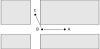
\includegraphics{transmision_misma_calle}
\decoRule
\caption[Transmisiones con línea de visión]{Transmisiones con línea de visión.}
\label{fig:transmision_misma_calle}
\end{figure}

Para lograr esto, cada vehículo debe poder saber qué vehículos se encuentran
circulando sobre su misma calle. Se puede considerar que, de cierta forma, los
paquetes recorren las calles a través de los vehículos. En la figura
\ref{fig:paquete_recorre_calle_1}, se muestra un paquete que es retransmitido
entre varios vehículos. En la figura \ref{fig:paquete_recorre_calle_2}, se
muestra el mismo escenario, pero se interpreta como el paquete recorriendo las
calles para moverse de un cruce vial a otro.

\begin{figure}[th]
\centering
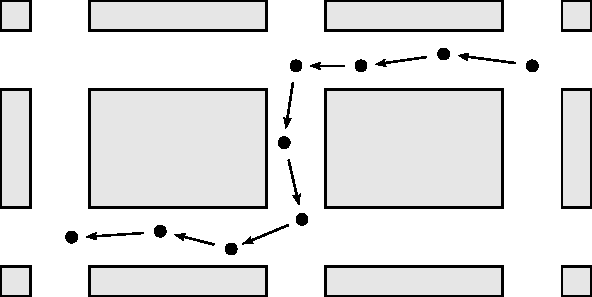
\includegraphics{paquete_recorre_calle_1}
\decoRule
\caption[Paquete siendo retransmitido entr vehículos]{Paquete siendo
retransmitido entre vehículos.}
\label{fig:paquete_recorre_calle_1}
\end{figure}

\begin{figure}[th]
\centering
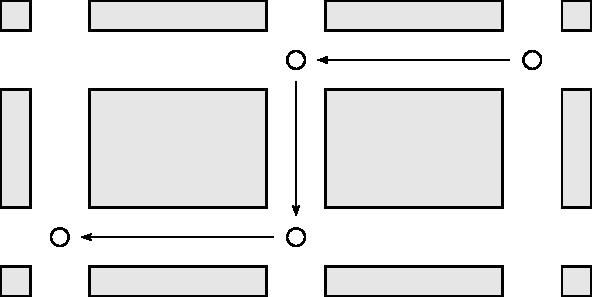
\includegraphics{paquete_recorre_calle_2}
\decoRule
\caption[Paquete recorriendo las calles]{Paquete recorriendo las calles.}
\label{fig:paquete_recorre_calle_2}
\end{figure}

Cuando un paquete llega al final de un segmento de calle y se encuentra en un
cruce vial, el vehículo portador debe determinar hacia qué calle debe seguir el
paquete para llegar a su destino, y seleccionar un vehículo que circule sobre
esa calle. En la figura \ref{fig:decision_cruce}, el vehículo B recibe un
paquete del vehículo A, y puede elegir entre tres calles para retransmitir el
paquete.

\begin{figure}[th!]
\centering
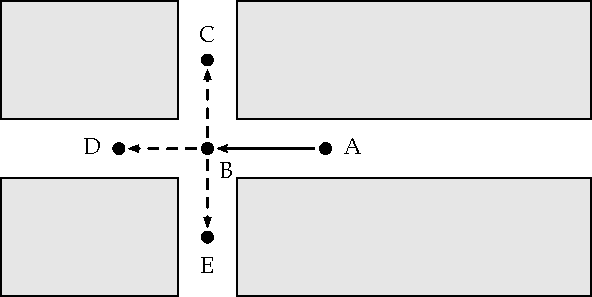
\includegraphics{decision_cruce}
\decoRule
\caption[Decisión de enrutamiento en cruce vial]{Decisión de enrutamiento en
cruce vial.}
\label{fig:decision_cruce}
\end{figure}

Para tomar este tipo de decisiones, se necesita que cada vehículo cuente con
información sobre la topología vial que le ayude a determinar cuál es la mejor
ruta. A continuación, se presenta cómo se estructura esta información y cómo se
utiliza durante el proceso de enrutamiento.

%-----------------------------------
%   GRAFO VIAL
%-----------------------------------
\section{Grafo vial}

\label{sec:grafo_vial}

En el protocolo propuesto, hay dos maneras de analizar el enrutamiento:
enrutamiento de red y enrutamiento vial. En el \keyword{enrutamiento de red},
se consideran los vehículos que conforman la ruta desde el origen hasta el
destino, y forman una \keyword{ruta de red}. En el \keyword{enrutamiento vial},
se consideran las calles que recorre un paquete para llegar a su destino, que
componen una \keyword{ruta vial}.

Para determinar una ruta vial, se define un grafo que represente la topología
vial para cada subred Geohash, denominado \keyword{grafo vial}, o \keyword{red
vial}. Se trata de un grafo no dirigido $\mathbf{G}=(\mathbf{V},\mathbf{E})$,
en el que $\mathbf{V}$ es el conjunto de vértices, que representan los cruces
viales, y $\mathbf{E}$ es el conjunto de aristas, que representan los segmentos
de las calles. La figura \ref{fig:grafo_vial_1} muestra el mapa de una región
Geohash, y su correspondiente grafo vial se muestra en la figura
\ref{fig:grafo_vial_2}.

\begin{figure}[th!]
\centering
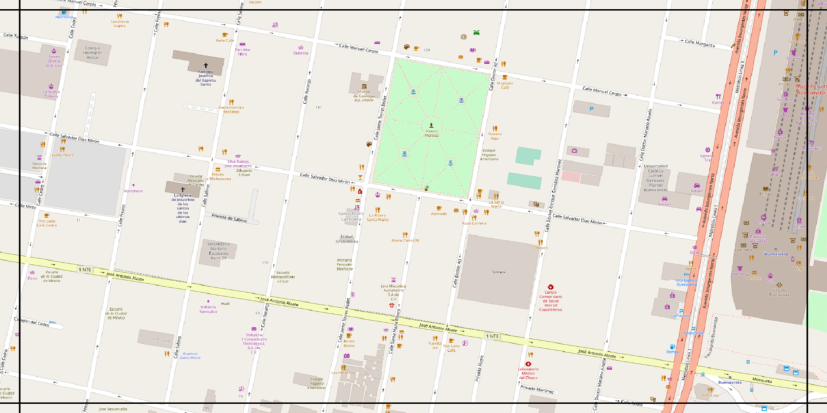
\includegraphics{grafo_vial_1} 
\decoRule
\caption[Región Geohash 9g3qxs]{Región Geohash 9g3qxs.}
\label{fig:grafo_vial_1}
\end{figure}

\begin{figure}[th!]
\centering
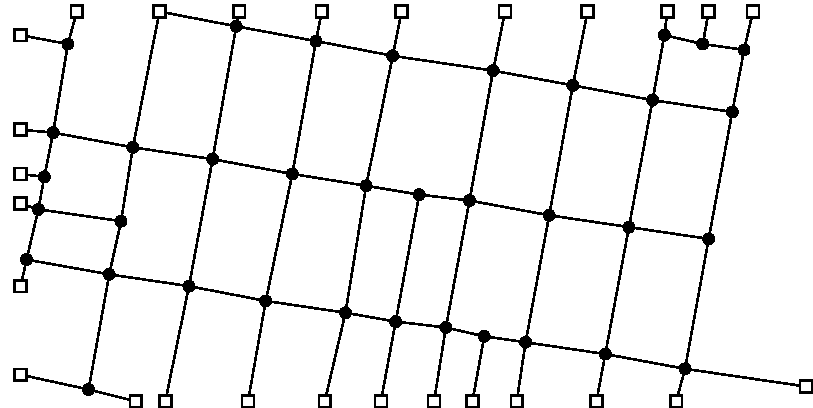
\includegraphics{grafo_vial_2} 
\decoRule
\caption[Grafo vial de la región Geohash 9g3qxs]{Grafo vial de la región
Geohash 9g3qxs.}
\label{fig:grafo_vial_2}
\end{figure}

Un grafo vial no pretende ser una representación fiel de la topología vial,
sino que se usa para determinar una ruta vial. Cada arista representa todos los
carriles que corresponden al segmento de calle que representa. Por otro lado,
cada vértice representa una ubicación en la que un vehículo puede transmitir
con posible línea de visión un paquete hacia los segmentos de calles que ahí
insiden. Por esta razón, los vértices son los puntos en los que los vehículos
toman decisiones de enrutamiento importantes.

En la sección \ref{sec:cambio_subred}, se usó el concepto de región
\textit{gateway} para explicar cómo un vehículo se autocofigura para unirse a
la subred adyacente y compartir paquetes entre ambas subredes. Sin emabargo, en
la realidad se utilizan los vértices del borde de un grafo vial para realizar
esta función, por lo que se denominan \keyword{vértices \textit{gateway}}, y se
muestran como cuadrados en la figura \ref{fig:grafo_vial_2}. De manera
similar, las aristas que tienen un vértice \textit{gateway} se denominan
\keyword{aristas \textit{gateway}}. Cuando un vehículo circula por una arista
\textit{gateway}, este asume que entró a la región \textit{gateway}, y realiza
el procedimiento descrito en la sección \ref{sec:cambio_subred}.

%-----------------------------------
%   ENRUTAMIENTO VIAL
%-----------------------------------
\section{Enrutamiento vial}

\label{sec:enrutamiento_vial}

Una \keyword{ruta vial} indica qué calles recorre un paquete para llegar a su
destino, y los vehículos que permiten que un paquete siga una ruta vial forman
una \keyword{ruta de red}. Debido a que los vehículos están en constante
movimiento, dos paquetes que sigan la misma ruta vial no necesariamente
seguirán la misma ruta de red.

Cuando el remitente y el destinatario se encuentran dentro de la misma región
Geohash, y, por lo tanto, pertenecen a la misma subred, se lleva a cabo lo que
se denomina \keyword{enrutamiento intrarregión}. En este caso, únicamente se
necesita conocer las calles que el paquete debe recorrer, que forman una
\keyword{ruta intrarregión}. Esto se traduce a determinar una ruta entre dos
vértices del grafo vial.

En la figura \ref{fig:enrutamiento_intrarregion}, un paquete debe llegar del
vehículo $V_1$ al vehículo $V_2$. Una ruta intrarregión que le permite al
paquete llegar al vehículo $V_2$ se muestra en la figura, y se forma por la
seuencia de vértices $h \rightarrow g \rightarrow f \rightarrow j$.

\begin{figure}[th!]
\centering
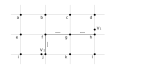
\includegraphics{enrutamiento_intrarregion}
\decoRule
\caption[Enrutamiento intrarregión]{Enrutamiento intrarregión.}
\label{fig:enrutamiento_intrarregion}
\end{figure}

Cuando el remitente y el destinatario se encuentran en regiones Geohash
diferentes, se debe realizar lo que se llama \textbf{enrutamiento interregión}.
Este consiste en determinar de qué subred a qué subred debe viajar un paquete
para llegar a la subred donde se encuentra el destino, lo que se denomina
\textbf{ruta interregión}. Cuando un paquete entra a una subred a través de un
vértice \textit{gateway}, se determina una ruta intrarregión que le permita
llegar a un vértice \textit{gateway} por el que pueda llegar a la siguiente
subred.

La figura \ref{fig:enrutamiento_interregion} muestra una ruta interregión que
indica por qué subredes debe pasar un paquete para llegar del vehículo $V_1$
al vehículo $V_2$. La ruta interregión se forma por las subredes 9g3qxm
$\rightarrow$ 9g3qxt $\rightarrow$ 9g3qxs $\rightarrow$ 9g3qxu.

\begin{figure}[th!]
\centering
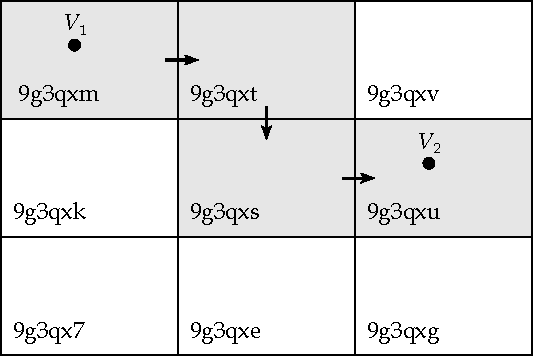
\includegraphics{enrutamiento_interregion}
\decoRule
\caption[Enrutamiento interregión]{Enrutamiento interregión.}
\label{fig:enrutamiento_interregion}
\end{figure}

%-----------------------------------
%   UBICACIÓN VIAL
%-----------------------------------
\section{Ubicación vial}

\label{sec:ubicacion_vial}

Los vehículos pueden conocer su ubicación en coordenadas geográficas (latitud y
longitud), así como la dirección y velocidad de su movimiento. No obstante,
para proporcionar información más útil a sus vecinos, cada vehículo también
necesita conocer su ubicación en el grafo vial de la subred donde se encuentra.
La \keyword{ubicación vial} de un vehículo indica en qué arista circula y su
distancia uno de los vértices de esta.

\begin{figure}[th!]
\centering
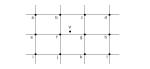
\includegraphics{ubicacion_vial_1} 
\decoRule
\caption[Vehículo en una red vial]{Vehículo en una red vial.}
\label{fig:ubicacion_vial_1}
\end{figure}

Las coordenadas de los vértices son conocidas, pero no se conoce el ancho de
cada calle, sino que se representan como segmentos de recta entre pares de
vértices. Es por esto que la ubicación del vehículo no cae exactamente sobre la
arista, sino en un punto cercano a esta. En la figura
\ref{fig:ubicacion_vial_1}, se muestra una red vial en la que hay un vehículo
en el puntio $V$.

\begin{figure}[th!]
\centering
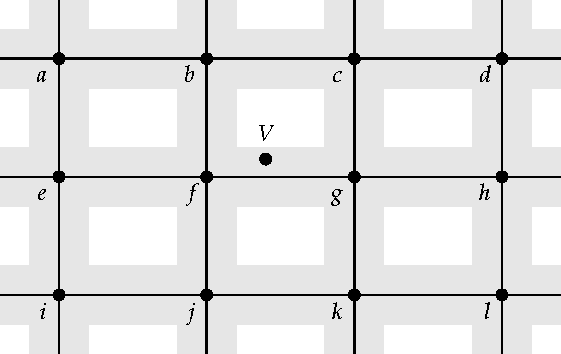
\includegraphics{ubicacion_vial_2} 
\decoRule
\caption[Dominio de las aristas en una red vial]{Dominio de las aristas en una
red vial.}
\label{fig:ubicacion_vial_2}
\end{figure}

La ubicación de un vehículo difícilmente cae exactamente sobre la arista
por donde circula, como se mencionó anteriormente. Por esta razón, se
consideta una región alrededor de la arista, denominada \keyword{dominio de la
arista}.  El dominio de una arista se delimita por dos líneas paralelas a la
arista, una a cada lado. En la figura \ref{fig:ubicacion_vial_2} se muestra el
dominio de cada arista, y se observa que el vehículo se encuentra dentro del
dominio de la arista $\{f,g\}$.

Si un vehículo se encuentra dentro del dominio de una arista, es posible que se
encuentre circulando por esta. Sin embargo, esta no es la única condición que
se debe cumplir para considerar que esto es verdad. Además de esto, la
dirección de su velocidad debe coincidir con la dirección de la arista. Cada
arista tiene dos direcciones, llamadas \keyword{direcciones de la arista}, como
se muestra en la figura \ref{fig:direcciones_arista}. Cada dirección es un
ángulo acimutal que indica hacia dónde se encuentra un vértice de la arista
respecto al otro.

\begin{figure}[th!]
\centering
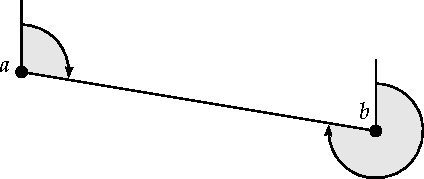
\includegraphics{direcciones_arista}
\decoRule
\caption[Direcciones de una arista]{Direcciones de una arista.}
\label{fig:direcciones_arista}
\end{figure}

Ya que cada vehículo es capaz de conocer la dirección de su movimiento, y las
direcciones de cada arista debido a que conoce la posición de sus vértices, se
puede determinar si estas coinciden. En la figura \ref{fig:ubicacion_vial_3} se
muestra que el vehículo se mueve en la misma dirección que la dirección del
vértice $g$ respecto al vértice $f$, y se encuentra dentro del dominio de la
arista $\{f,g\}$, por lo que se considera que está circulando sobre esa arista.

\begin{figure}[th!]
\centering
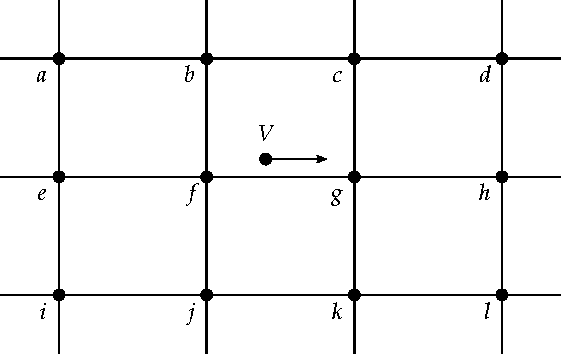
\includegraphics{ubicacion_vial_3} 
\decoRule
\caption[Dirección del movimiento de un vehículo en una red vial]{Dirección del
movimiento de un vehículo en una red vial.}
\label{fig:ubicacion_vial_3}
\end{figure}

Además de conocer en qué arista se encuentra circulando un vehículo, se
necesita saber en qué posición se encuentra circulando en dicha arista. Para
esto, se obtiene la proyección de la ubicación del vehículo en la arista y se
calcula su distancia a uno de los dos vértices, como se muestra en la figura
\ref{fig:ubicacion_vial_4}, donde se muestra la distancia al vértice $f$.

\begin{figure}[th!]
\centering
\includegraphics{ubicacion_vial_4} 
\decoRule
\caption[Posición de un vehículo en una red vial]{Posición de un vehículo en
una arista.}
\label{fig:ubicacion_vial_4}
\end{figure}

La ubicación vial de un vehículo consiste en los dos vértices de la arista
por la que circula y su posición en esta arista, es decir la distancia de su
proyección en la arista al primer vértice. Además, si su distancia a alguno de
los dos vértices de la arista es menor a un límite, cuyo valor se define por el
parámero RADIO\_CERCANIA\_VERTICE, se considera que \keyword{el vehículo se
encuentra en el vértice}.

%-----------------------------------
%   CABECERAS DE OPCIONDES DE SALTO POR SALTO
%-----------------------------------
\section{Cabecera de opciones de salto por salto}

\label{sec:cabecera_opciones}

Los paquetes deben incluir información que permita a los vehículos tomar
decisiones de enrutamiento. Las cabeceras de extensión sirven para incluir
información opcional adicional en un datagrama. La función de la
\keyword{cabecera de opciones de salto por salto} es contener información que
toods los enrutadores (vehículos en este caso) puedan revisar. Por esta razón,
esta cabecera se usa para incluir la información de enrutamiento en el paquete.
La figura \ref{fig:formato_datagrama_ipv6_cabecera} muestra la estructura del
datagrama IPv6 con la cabecera de opciones de salto por salto, y el formato de
esta cabecera se muestra en la figura
\ref{fig:formato_cabecera_salto_por_salto} \cite{RFC2460}.

\begin{figure}[th!]
\centering
\includegraphics{formato_datagrama_ipv6_cabecera} 
\decoRule
\caption[Datagrama IPv6 con la cabecera de opciones de salto por
salto]{Datagrama IPv6 con la cabecera de opciones de salto por salto.}
\label{fig:formato_datagrama_ipv6_cabecera}
\end{figure}

\begin{figure}[th!]
\centering
\includegraphics{formato_cabecera_salto_por_salto}
\decoRule
\caption[Formato de la cabecera de salto por salto]{Formato de la cabecera de
salto por salto.}
\label{fig:formato_cabecera_salto_por_salto}
\end{figure}

Los campos de la cabecera de opciones de salto por salto son los siguientes:

\keyword{Siguiente cabecera (8 bits)} -- Identifica el tipo de cabecera que
sigue después.

\keyword{Longitud de la cabecera (8 bits)} -- Longitud, en unidades de 8
octetos, de la cabecera de salto por salto, sin incluir los primeros 8 bytes.

\keyword{Opciones (longitud variable)} -- Secuencia de opciones que se procesan
en cada enrutador. Su longitud debe ser tal que la longitud total de la
cabecera de salto por salto sea un múltiplo entero de 8 octetos.

Las opciones se codifican con el formato tipo-longitud-valor (TLV), que se
muestra en la figura \ref{fig:formato_tlv}. Los campos de cada opción son los
siguientes \cite{RFC2460}:

\begin{figure}[th!]
\centering
\includegraphics{formato_tlv}
\decoRule
\caption[Formato TLV]{Formato TLV.}
\label{fig:formato_tlv}
\end{figure}

\keyword{Tipo (8 bits)} -- Identificador del tipo de opción.

\keyword{Longitud del valor (8 bits)} -- Longitud en octetos del campo del
valor del dato.

\keyword{Valor (longitud variable)} -- Valor de la opción.

En el tipo de opción, los dos primeros bits indican qué hacer si la opción no
es reconocida, y el tercer bit indica si el valor del dato puede cambiar o no a
lo largo de la ruta.

%-----------------------------------
%   OPCIÓN DE UBICACIÓN DEL DESTINO
%-----------------------------------
\subsection{Opción de ubicación del destino}

\label{subsec:opcion_de_ubicacion_del_destino}

Para poder enrutar un paquete, el \textit{host} que lo origina agrega la
\keyword{opción de ubicación del destino} a la cabecera de opciones de salto
por salto. El formato de la opción de ubicación del destino se muestra en la
figura \ref{fig:formato_opcion_ubicacion_destino}, y contiene los siguientes
campos:

\begin{figure}[th!]
\centering
\includegraphics{formato_opcion_ubicacion_destino}
\decoRule
\caption[Formato de la opción de ubicación del destino]{Formato de la opción de
ubicación del destino.}
\label{fig:formato_opcion_ubicacion_destino}
\end{figure}

\keyword{Tipo (8 bits)} -- El tipo de la opción es 88, donde los primeros dos
bits indican que el paquete debe ser descartado si no se reconoce el tipo de
opción, y el tercer bit indica que el valor de la opción no cambia a lo largo
de la ruta.

\keyword{Longitud del valor (8 bits)} -- La longitud del valor es de 8 octetos.

\keyword{Ubicación Geohash (64 bits)} -- Ubicación Geohash de longitud 12 del
\textit{host} de destino.

%-----------------------------------
%   OPCIÓN DE UBICACIÓN VIAL DEL DESTINO
%-----------------------------------
\subsection{Opción de ubicación vial del destino}

\label{subsec:opcion_de_ubicacion_vial_del_destino}

Cuando un vehículo recibe un paquete, puede revisar la opción de ubicación del
destino para saber la ubicación geográfica a donde este tiene que llegar. Sin
embargo, para calcular una ruta vial, también se debe conocer la ubicación vial
destino.

Si un vehículo recibe un paquete cuyo destino se encuentra en la misma subred,
debe calcular la ubicación vial del destino y agregarla a la cabecera de
opciones con la \keyword{opción de ubicación vial del destino}. El formato de
este tipo de opción se muestra en la figura
\ref{fig:formato_opcion_ubicacion_vial_destino}, y contiene los siguientes
campos:

\begin{figure}[th!]
\centering
\includegraphics{formato_opcion_ubicacion_vial_destino}
\decoRule
\caption[Formato de la opción de ubicación vial del destino]{Formato de la
opción de ubicación vial del destino.}
\label{fig:formato_opcion_ubicacion_vial_destino}
\end{figure}

\keyword{Tipo (8 bits)} -- El tipo de la opción es 25, donde los primeros dos
bits indican que la opción se ignora si no se reconoce el tipo de opción, y el
tercer bit indica que el valor no cambia a lo largo de la ruta.

\keyword{Longitud del valor (8 bits)} -- La longitud del valor es de 6 octetos.

\keyword{Vértice 1 (16 bits)} -- Vértice 1 de la arista donde se ecuentra el
destino.

\keyword{Vértice 2 (16 bits)} -- Vértice 2 de la arista donde se ecuentra el
destino.

\keyword{Distancia 1 (16 bits)} -- Valor entero de la distancia en metros al
vértice 1.

Si un el destino un paquete se encuentra en una subred diferente a la subred en
la que se encuentra, no necesita llevar esta opción, ya que primero se debe
enrutar entre las subredes hasta llegar a la correspondiente. El primer
vehículo que recibe el paquete y se encuentra en la misma subred que el destino
se encarga de agregar esta opción.

%-----------------------------------
%   OPCIÓN DE VÉRTICES VISITADOS
%-----------------------------------
\subsection{Opción de vértices visitados}

\label{subsec:opcion_de_vertices_visitados}

Para evitar que un paquete pase más de una vez por el mismo vértice, debe
llevar un registro de los vértices por los que ha pasado. Estos se indican en
la \keyword{opción de vértices visitados}. El formato de esta opción se indica
en la figura \ref{fig:formato_opcion_vertices_visitados}, y contiene los
siguientes campos:

\begin{figure}[th!]
\centering
\includegraphics{formato_opcion_vertices_visitados}
\decoRule
\caption[Formato de la opción de vértices visitados]{Formato de la opción de
vértices visitados.}
\label{fig:formato_opcion_vertices_visitados}
\end{figure}

\keyword{Tipo (8 bits)} -- El tipo de la opción es 58, donde los primeros dos
bits indican que la opción se ignora si no se reconoce el tipo de opción, y el
tercer bit indica que el valor puede cambiar a lo largo de la ruta.

\keyword{Longitud del valor (8 bits)} -- La longitud del valor es variable.

\keyword{Vértices visitados (longitud variable)} -- Lista de vértices por los
que el paquete ha pasado. Cada vértice ocupa 2 octetos.

La opción de vértices visitados sólo es válida dentro de una subred. Cuando un
paquete pasa de una subred a otra, se elimina la opción de vértices visitados
de la cabecera y se agrega una nueva para los vértices de la siguiente subred.

%-----------------------------------
%   FORMATO DE LOS MENSAJES
%-----------------------------------
\section{Formato de los mensajes}

\label{sec:formato_mensajes}

Los tipos de mensajes que define el protocolo propuesto son
anuncio-\textit{host} (ANC-HOST), anuncio-vehículo (ANC-VEHIC),
\textit{ping}-vértice (PING), \textit{pong}-vértice (PONG) Estos mensajes se
transmiten mediante el protocolo UDP, y no requieren ningún tipo de
procesamiento especificado en alguna cabecera IPv6.

Los vehículos necesitan anunciar su presencia y su ubicación ante sus vecinos
mediante la transmisión de mensajes ANC-VEHIC periódicamente. Esto sirve para
que los vecinos sepan que sigue activo el enlace hacia este. Si pasa cierta
cantidad de tiempo desde la última vez que se recibió un mensaje ANC-VEHIC de
un vehículo, se asume que el enlace se perdió.

Los mensajes ANC-HOST son transmitidos por los \textit{hosts} para anunciar su
presencia ante los vehículos vecinos. Cuando un vehículo debe entregar un
paquete a un \textit{host}, y éste recibió recientemente un mensaje ANC-HOST de
este \textit{host}, le envía el paquete directamente en lugar de enrutarlo
hacia otro vehículo.

Las rutas que determina este protocolo indican qué aristas debe recorrer un
paquete para llegar a su destino. Sin embargo, encontrar una ruta vial no
garantiza que a lo largo de toda la ruta haya vehículos por los que pueda pasar
el paquete desde el inicio hasta el final. Para saber si un paquete puede
atravesar una arista, se lleva a cabo una operación denominada
\keyword{ping-pong}. Esta consiste en enviar un mensaje PING desde un vértice
de una arista y verificar que llegue al otro vértice. Si este mensaje puede
llegar, se responde enviando un mensaje PONG de regreso. De esta manera, se
verifica si un paquete puede atravesar dicha arista.

En las siguientes secciones, se describe el formato de cada uno de los tipos de
mensajes.

%-----------------------------------
%   MENSAJE ANUNCIO-VEHÍCULO
%-----------------------------------
\subsection{Anuncio-vehículo (ANC-VEHIC)}

\label{subsec:mensaje_anc_vehic}

El formato del mensaje anuncio se muestra en la figura
\ref{fig:formato_anc_vehic}, y contiene los siguientes campos:

\begin{figure}[th!]
\centering
\includegraphics{formato_anc_vehic}
\decoRule
\caption[Formato del mensaje ANC-VEHIC]{Formato del mensaje ANC-VEHIC.}
\label{fig:formato_anc_vehic}
\end{figure}

\keyword{Tipo (8 bits)} -- Su valor es \code{1} para indicar que se trata de un
mensaje ANC-VEHIC.

\keyword{P (1 bit)} -- Indica si el mensaje anuncia el resultado de una
operación ping-pong.

\keyword{E (1 bit)} -- Si vale 1, indica que hubo un error en la operación
ping-pong, lo que significa que la arista que se anuncia está inactiva.
Únicamente se considera si la bandera \keyword{P} vale 1.

\keyword{V (1 bit)} -- Si vale 0, el campo \keyword{vértice 1} indica el
vértice donde se inició la operación ping-pong. Si vale 1, se trata del campo
\keyword{vértice 2}. Únicamente se considera si la bandera \keyword{P} vale 1.

\keyword{Dirección (16 bits)} -- Ángulo acimutal de la dirección del movimiento
del vehículo en grados.

\keyword{Velocidad (16 bits)} -- Velocidad del vehículo en m/s.

\keyword{Vértice 1 (16 bits)} -- Vértice 1 de la arista por la que
circula el vehículo. Es el vértice hacia el que se dirige el vehículo.

\keyword{Vértice 2 (16 bits)} -- Vértice 2 de la arista por la que
circula el vehículo.

\keyword{Distancia 1 (16 bits)} -- Valor entero de la distancia en metros del
vehículo al vértice 1.

\keyword{Dirección IPv6 (128 bits)} -- Dirección del vehículo que emite el
mensaje.

\keyword{Ubicación Geohash (64 bits)} -- Ubicación Geohash de longitud 12 al
momento de emitir el mensaje.

%-----------------------------------
%   MENSAJE ANUNCIO-HOST
%-----------------------------------
\subsection{Anuncio-\textit{host} (ANC-HOST)}

\label{subsec:mensaje_anuncio_host}

El formato del mensaje ANC-HOST se muestra en la figura
\ref{fig:formato_anc_host}, y contiene los siguientes campos:

\begin{figure}[th!]
\centering
\includegraphics{formato_anc_host}
\decoRule
\caption[Formato del mensaje ANC-HOST]{Formato del mensaje ANC-HOST.}
\label{fig:formato_anc_host}
\end{figure}

\keyword{Tipo (8 bits)} -- Su valor es \code{2} para indicar que se trata de un
mensaje ANC-HOST.

\keyword{Dirección IPv6 (128 bits)} -- Dirección del \textit{host} que emite el
mensaje.

\keyword{Ubicación Geohash (65 bits)} -- Ubicación del \textit{host} al momento
de emitir el mensaje.

%-----------------------------------
%   MENSAJE PING
%-----------------------------------
\subsection{Ping (PING)}

\label{subsec:mensaje_ping}

El formato del mensaje PING se muestra en la figura \ref{fig:formato_ping}, y
contiene los siguientes campos:

\begin{figure}[th!]
\centering
\includegraphics{formato_ping}
\decoRule
\caption[Formato del mensaje PING]{Formato del mensaje PING.}
\label{fig:formato_ping}
\end{figure}

\keyword{Tipo (8 bits)} -- Su valor es \code{3} para indicar que se trata de un
mensaje PING.

\keyword{Vértice 1 (16 bits)} -- Vértice de origen.

\keyword{Vértice 2 (16 bits)} -- Vértice de destino.

\keyword{Dirección IPv6 (128 bits)} -- Dirección del vehículo que originó el
mensaje.

%-----------------------------------
%   MENSAJE PONG
%-----------------------------------
\subsection{Pong (PONG)}

\label{subsec:mensaje_pong}

El formato del mensaje PONG se muestra en la figura \ref{fig:formato_pong}, y
contiene los siguientes campos:

\begin{figure}[th!]
\centering
\includegraphics{formato_pong}
\decoRule
\caption[Formato del mensaje PONG]{Formato del mensaje PONG.}
\label{fig:formato_pong}
\end{figure}

\keyword{Tipo (8 bits)} -- Su valor es \code{4} para indicar que se trata de un
mensaje PONG.

\keyword{E (1 bit)} -- Bandera de error. Si vale \code{1}, indica que hubo un
error en la operación ping-pong.

\keyword{Vigencia (16 bits)} -- Tiempo de vigencia, en milisegundos, restante
del último mensaje PONG recibido.

\keyword{Vértice 1 (16 bits)} -- Vértice de origen del mensaje PING que
responde.

\keyword{Vértice 2 (16 bits)} -- Vértice de destino del mensaje PING que
responde.

\keyword{Dirección IPv6 (128 bits)} -- Dirección del vehículo que originó el
mensaje PING que responde.

%-----------------------------------
%   DIRECTORIO DE VEHÍCULOS VECINOS
%-----------------------------------
\section{Directorio de vehículos vecinos}

\label{sec:directiorio_vehiculos_vecinos}

\begin{sloppypar}
Los vehículos informan sobre su disponibilidad por medio de mensajes
\mbox{ANC-VEHIC}, en los que se incluye información sobre su ubicación vial. La
frecuencia con la que los vehículos transmiten estos mensajes se determina con
el parámetro \mbox{INTERVALO\_ANC\_VEHIC}. Para que todos los vehículos puedan
recibir estos mensaje, éste se dirige a la dirección \textit{multicast} de la
subred.
\end{sloppypar}

Cada vehículo tiene un \keyword{directorio de vehículos vecinos}, que le
permite mantener un registro de los vehículos que se encuentran cerca. Esta
información le ayuda a determinar el siguiente salto al enrutar un paquete.
Cada registro en el directorio de vehículos vecinos contiene los siguientes
campos:

\begin{center}
\begin{tabular}{ r l }
Dirección IP: & Tiempo de expiración \\
& Ubicación \\
& Velocidad \\
& Dirección de movimiento \\
& Vértice A \\
& Vértice B \\
& Distancia a A \\
& Distancia a B
\end{tabular}
\end{center}

Cada registro se identifica con la dirección IP del vehículo, y los campos de
cada registro son los siguientes:

\keyword{Tiempo de exporación} -- Tiempo hasta el que el registro es válido.

\keyword{Ubicación Geohash} -- Ubicación del vehículo.

\keyword{Velocidad} -- Velocidad del vehículo en m/s.

\keyword{Dirección del movimiento} -- Ángulo acimutal de la dirección del
movimiento del vehículo en grados.

\keyword{Vértice A} -- Primer vértice de la arista por la que
circula el vehículo. Es el vértice hacia el que se dirige el vehículo.

\keyword{Vértice B} -- Segundo vértice de la arista por la que
circula el vehículo.

\keyword{Distancia A} -- Distancia al vértice A.

\keyword{Distancia B} -- Distancia al vértice B.

\begin{sloppypar}
Cuando un vehículo recibe un mensaje ANC-VEHIC, obtiene la ubicación vial del
vecino. Si no hay un registro con la dirección IP, se crea uno nuevo, y si ya
existe, se actualiza el registro. El tiempo de expiración se obtiene a partir
del valor del parámetro VIGENCIA\_VEHICULO\_VECINO, y se actualiza cada vez que
llega un mensaje del vehículo correspondiente.
\end{sloppypar}

Si un vehículo deja de recibir mensajes ANC-VEHIC de otro, el tiempo de
expiración del registro deja de actualizarse, y cuando se cumple este tiempo,
se asume que el enlace hacia tal vehículo se terminó y se elimina el registro.

%-----------------------------------
%   DIRECTORIO DE HOSTS VECINOS
%-----------------------------------
\section{Directorio de \textit{hosts} vecinos}

\label{sec:directorio_hosts_vecinos}

De manera similar, los \textit{hosts} que necesiten comunicarse a través de
la VANET se anuncian ante los vehículos vecinos. Esto lo hacen enviando su
dirección IP y su ubicación en mensajes ANC-HOST a la dirección
\textit{multicast}. La frecuencia con la que un \textit{host} transmite estos
mensajes se especifica con el parámetro INTERVALO\_ANC\_HOST

Únicamente los vehículos pueden procesar los mensajes ANC-HOST, y tienen un
\keyword{directorio de hosts vecinos}, donde registran los \textit{hosts} de
los que han recibido algún mensaje ANC-VEHIC recientemente. Cada registro
contiene los siguientes datos:

\begin{center}
\begin{tabular}{ r l }
Dirección IP: & Tiempo de expiración \\
& Ubicación \\
\end{tabular}
\end{center}

Los campos de cada registro del directorio son los siguientes:

\keyword{Tiempo de exporación} -- Tiempo hasta el que el registro es válido.

\keyword{Ubicación} -- Ubicación del \textit{host}.

Al igual que en el directorio de vehículos vecinos, cada registro tiene un
tiempo de validez, que se define con el parámetro VIGENCIA\_HOST\_VECINO, y se
actualiza cada vez que se recibe un mensaje ANC-HOST. Si se cumple el tiempo de
expiración de un registro, este se elimina.

%-----------------------------------
%   PING-PONG
%-----------------------------------
\section{Operación ping-pong}

\label{sec:operacion_ping_pong}

Tener una ruta vial no significa que existan vehículos en todas la aristas a
lo largo de la ruta. Por lo tanto, es importante verificar si en una arista hay
vehículos que puedan retransmitir un paquete para que llegue al otro extremo de
esta. La operación ping-pong sirve para verificar si se cumple esta condición
en una arista.

Una operación ping-pong comienza cuando un vehículo que se encuentra en un
vértice origina un mensaje PING, el cual retransmite hacia algún vehículo
vecino que se encuentra en la arista de interés, si es que hay. En este
mensaje, el campo \keyword{vértice 1} indica el vértice donde se inicia la
operación, y el vértice al que debe llegar se indica en el campo
\keyword{vértice 2}. El mensaje también lleva la dirección IP del vehículo que
lo originó. La figura \ref{fig:recorrido_ping} muestra el recorrido de un
mensaje PING para llegar de un vértice al otro.

\begin{figure}[th!]
\centering
\includegraphics{recorrido_ping}
\decoRule
\caption[Recorrido de un mensaje PING]{Recorrido de un mensaje PING.}
\label{fig:recorrido_ping}
\end{figure}

El mensaje PING se retransmite entre los vehículos hasta llegar a alguno que se
encuentre en el otro vértice de la arista. Este vehículo responde con un
mensaje PONG, que se retransmite de regreso hasta llegar al vehículo que inició
la operación. En este mensaje, la bandera \keyword{E} tiene un valor de 0, para
indicar que el mensaje PING llegó al vértice. El campo \keyword{vértice 1}
indica el vértice donde se originó el mensaje PING, y el campo \keyword{vértice
2} indica el vértice al que tenía que llegar. En la figura
\ref{fig:recorrido_pong} se muestra el recorrido de un mensaje PONG para llegar
al vehículo que inició la operación.

\begin{figure}[th!]
\centering
\includegraphics{recorrido_pong}
\decoRule
\caption[Recorrido de un mensaje PONG]{Recorrido de un mensaje PONG.}
\label{fig:recorrido_pong}
\end{figure}

Si un vehículo recibe un mensaje PING pero no encuentra un vecino al que
retransmitirlo, éste responde con un mensaje PONG, asignando el valor 1 a la
bandera \keyword{E} para indicar que no se completó la operación, lo que
significa que el vértice de destino no se puede alcanzar.

Cuando un vehículo que inició la operación recibe el mensaje PONG de respuesta,
y la bandera de error \keyword{E} tiene un valor de 0, se dice que la arista es
una \keyword{arista activa}. En este caso, el vehículo transmite un mensaje
ANC-VEHIC, en el que la bandera \keyword{P} tiene el valor 1 para anunciar el
resultado de una operación ping-pong, el vértice de destino de la operación se
indica en el campo \keyword{vértice ping-pong}, y la bandera \keyword{E} tiene
valor de 0 para decir que la arista está activa. Este mensaje también incluye
la ubicación vial del vehículo, igual que los mensajes ANC-VEHIC que se
transmiten periódicamente.

El vehículo que inicia una operación ping-pong establece un tiempo de espera,
definido por el parámetro ESPERA\_PONG. Si el tiempo de espera se agota, o si
recibe un mensaje PONG de respuesta con el valor 1 en la bandera de error
\keyword{E}, se transmite un mensaje ANC-VEHIC, pero con la bandera \keyword{E}
con el mismo valor para anunciar que la arista está inactiva.

Cuando el mensaje PING logra atravesar la arista y llega a un vehículo en el
vértice deseado, después de responder con el mensaje PONG, este vehículo
también anuncia, con un mensaje ANC-VEHIC, que la arista está activa.

%-----------------------------------
%   ARISTAS ACTIVAS E INACTIVAS
%-----------------------------------
\subsection{Aristas activas e inactivas}

\label{subsec:aristas_activas_e_inactivas}

Con la operación ping-pong es posible saber si hay vehículos que puedan
retransmitir paquetes de un vértice a otro. Esto es importante a la hora del
cálculo de las rutas viales, por lo que cada vehículo tiene un registro de
aristas activas y otro de aristas inactivas.

Cuando se recibe un mensaje ANC-VEHIC que indica el resultado de una operación
ping-pong, se revisa el campo \keyword{vértice ping-pong} y la bandera
\keyword{V} para saber de qué arista se trata, y se agrega al \keyword{registro
de aristas activas}, junto con su tiempo de validez determinado por el
parámetro VIGENCIA\_ARISTA\_ACTIVA. Si la arista ya está registrada, se
actualiza el tiempo de validez. Se asume que la arista está activa hasta que
se agota el tiempo de validez. Una vez que se agota, se elimina del registro y
se desconoce el estado de la arista, hasta la siguiente actualización.

Si se recibe un mensaje ANC-VEHIC una arista inactiva, se revisa para saber de
qué arista se trata, y se agrega al \keyword{registro de aristas inactivas}
junto con un tiempo de validez definido por el parámetro
VIGENCIA\_ARISTA\_INACTIVA. Si ya la arista vértice ya existe en el registro,
se actualiza el tiempo de validez. Si este tiempo se agota, se elimina del
registro.

%-----------------------------------
%   ENRUTAMIENTO
%-----------------------------------
\section{Enrutamiento}

\label{sec:enrutamiento}

En las siguientes secciones, se presenta el proceso que lleva a cabo un vehículo
cuando recibe un paquete para enrutar.

%-----------------------------------
%   CÓMPUTO DE RUTAS VIALES
%-----------------------------------
\subsection{Cómputo de rutas viales}

\label{subsec:computo_rutas_viales}

Para tratar de evitar pérdida de paquetes por obstrucciones de edificios, se
busca que las rutas incluyan la menor cantidad de giros en esquinas posible.
En la figura \ref{fig:ruta_mala} se muestra una ruta del vértice $d$ al vértice
$i$ en la que hay giros en cuatro esquinas. Si un paquete siguiera esa ruta, en
cada uno de los giros habría posibilidad de chocar con el edificio de la
esquina.

\begin{figure}[th!]
\centering
\includegraphics{ruta_mala}
\decoRule
\caption[Ruta con muchos giros en esquinas]{Ruta con muchos giros en
esquinas.}
\label{fig:ruta_mala}
\end{figure}

En cambio, en la figura \ref{fig:ruta_buena} se muestra otra ruta que une los
mismos vértices, pero esta únicamente incluye un giro. Si un paquete siguiera
esta ruta, sólo correría el riesgo de chocar con algún edificio en un giro. Por
esta razón, la busqueda de rutas viales debe considerar tramos rectos lo más
largos que sea posible.

\begin{figure}[th!]
\centering
\includegraphics{ruta_buena}
\decoRule
\caption[Ruta con un giro en una esquinas]{Ruta con un giro en una
esquinas.}
\label{fig:ruta_buena}
\end{figure}

Para utilizar un algoritmo para determinar las rutas en el grafo vial, es
necesario asignar un peso a cada una de las aristas. Sin embargo, para generar
rutas con el criterio descrito anteriormente, el peso de cada arista depende de
la arista anterior. Por ejemplo, en la ruta de la figura \ref{fig:ruta_mala},
para ir de la arista $\{d,c\}$ a la arista $\{c,g\}$, hay un giro de ángulo
considerable, mientras que en la ruta de la figura \ref{fig:ruta_buena}, para
ir de la arista $\{d,c\}$ a la arista $\{c,b\}$, el tramo es recto, por lo que
la arista $c,b\}$ tendrá un peso menor que la arista $d,g\}$ respecto a la
arista $\{d,c\}$.

Existen algoritmos para grafos que calculan la ruta más corta desde un vértice
inicial al resto de los vértices, como el algoritmo de Dijkstra
\cite{cormen2001}. Sin embargo, este algoritmo asume que las aristas tienen un
peso fijo previamente asignado. Por este motivo, se propone un algoritmo
inspirado en el algoritmo de Dijkstra, pero que hace la búsqueda de las rutas a
partir de los dos vértices de una arista inicial. Además, el peso de cada
arista se calcula conforme el algoritmo progresa, y descarta un conjunto de
aristas inactivas y los vértices por los que el paquete ya ha pasado.

En la figura \ref{fig:angulos_aristas}, la flecha indica la dirección de la
arista $\{a,b\}$, y se muestran los ángulos que forma esta con la dirección de
cada una de las demás aristas. Estos ángulos van a funcionar como el peso de su
respectiva arista. Debido a que $\{b,d\}$ forma el menor ángulo con la
dirección de $\{a,b\}$, ésta tiene el menor peso, y $\{b,c\}$ tendrá el mayor
peso, ya que su ángulo es el mayor. De este modo, la ruta contendrá la menor
cantidad de giros pronunciados en los cruces viales.

\begin{figure}[th!]
\centering
\includegraphics{angulos_aristas}
\decoRule
\caption[Determinación del peso de las aristas con sus ángulos de
dirección]{Determinación del peso de las aristas con sus ángulos de dirección.}
\label{fig:angulos_aristas}
\end{figure}

\begin{algorithm}[th!]
\small
\caption{Cálculo de la ruta más corta}
\label{alg:ruta_mas_corta}
\DontPrintSemicolon
\LinesNumbered
    \KwData{$\{a,b\}$: Arista inicial, $\mathbf{G}$: Grafo vial, $VV$: Conjunto
    de vértices visitados, $AE$: Conjunto de aristas activas}
    \Begin{
        \ForEach{$v \in \mathbf{G}.\mathbf{V}$} {
            $distancias[v] \gets \infty$ \;
        }
        $distancias[a] \gets 0$ \;
        $distancias[b] \gets 0$ \;
        $S \gets \mathbf{G.V} \setminus \{a,b\}$ \;
        \ForEach{$v \in \mathbf{G}.\mathbf{V}$ adyacente a $a$}{
            \If{$v \neq b$}{
                \eIf{$v \notin VV$ y $\{a,v\} \in AE$}{
                    $distancias[v] \gets calcularPeso(\{a,v\}, \{a,b\})$ \;
                    $predecesores[v] \gets a$ \;
                }{
                    $S \gets S \setminus \{v\}$ \;
                }
            }
        }
        \ForEach{$v \in \mathbf{G}.\mathbf{V}$ adyacente a $b$}{
            \If{$v \neq a$}{
                \eIf{$v \notin VV$ y $\{b,v\} \in AE$}{
                    $peso \gets calcularPeso(\{b,v\}, \{a,b\}$) \;
                    \If{$peso < distancias[v]$}{
                        $distancias[v] \gets peso$ \;
                        $predecesores[v] \gets b$ \;
                    }
                }{
                    $S \gets S \setminus \{v\}$ \;
                }
            }
        }
        \While{$S \neq \emptyset$}{
            $v \gets$ vértice en $S$ con menor distancia \;
            $u \gets predecesores[v]$ \;
            \ForEach{$w \in \mathbf{G}.\mathbf{V}$ adyacente a $v$}{
                \If{$w \neq u$}{
                    \eIf{$w \notin VV$}{
                        $peso \gets calcularPeso(\{v,w\}, \{u,v\})$ \;
                        \If{$distancias[w] > distancias[v] + peso$}{
                            $distancias[w] \gets distancias[v] + peso$ \;
                            $predecesores[w] \gets v$ \;
                        }
                    }{
                        $S \gets S \setminus \{w\}$ \;
                    }
                }
            }
            $S \gets S \setminus \{v\}$ \;
        }
        \Return{predecesores, distancias}
    }
\end{algorithm}

El algoritmo \ref{alg:ruta_mas_corta} es el algoritmo propuesto, donde se
definen dos vectores cuyo tamaño es igual al número de vértices en el grafo. El
vector $predecesores$ indica cuál es el vértice predecesor de cada uno en la
ruta. El vector $distancias$ indica la distancia desde la arista de inicia
hacia cada vértice. En este contexto, se entiende como distancia a la suma de
los pesos de todas las aristas que forman una ruta, por lo que se denomina
\keyword{distancia de ruta}, para evitar confusión. También se define un
conjunto llamado $S$, que contiene los vértices cuya ruta falta obtener.

El algoritmo recibe la arista inicial $\{a,b\}$, el grafo vial $\mathbf{G}$,
el conjunto de vértices no disponibles $NV$ y el conjunto de aristas inactivas
$NE$. En las líneas 3-6, se establece la distancia de ruta a cada vértice como
$\infty$, excepto para los vértices iniciales, cuya distancia de ruta es 0. En
la línea 7 se agregan todos los vértices a $S$, excepto los dos iniciales.

En las líneas 8-12, se calcula y actualiza la distancia de ruta a los vértices
adyacentes a $a$, excepto los vétices no disponibles. En las líneas 13-19, se
hace el mismo procedimiento, pero para los vértices adyacentes a $b$, y después
se procede a procesar el resto de los vértices. Debido a que la distancia de
ruta de los vértices no disponibles nunca deja de ser $\infty$, en la línea 21
se verifica si existe un vértice $u$ en $S$ cuya distancia de ruta ya se haya
calculado anteriormente, es decir, que se puede alcanzar mediante un vértice ya
procesado. Si no hay, se termina el algoritmo, pero si sí hay, se calcula la
distancia de ruta hacia cada uno de sus vértices adyacentes, y se actualiza si
es una distancia de ruta menor a la que ya tenía, en cuyo caso, se asigna $u$
como su predecesor.

El resultado final son los vectores $predecesores$ y $distancias$. Con el
vector $predecesores$, para determinar la ruta hacia un vértice $u$, se busca
su predecesor $v$. Después, se busca $v$ y se obtiene su predecesor $w$, y esto
se repite hasta llegar a alguno de los dos vértices iniciales. Con el vector
$distancias$ se puede saber si se encontró alguna ruta hacia cierto vértice. Si
su distancia de ruta es $\infty$, significa que no se encontró.

%-----------------------------------
%   VERIFICACIÓN DE LA CABECERA DE OPCIONES DE SALTO POR SALTO
%-----------------------------------
\subsection{Verificación de la cabecera de opciones de salto por salto}

\label{subsec:verificacion_cabecera_opciones_salto_por_salto}

Cuando un vehículo recibe un paquete, primero debe verificar si este contiene
la cabecera de opciones de salto por salto. De ser así, verifica si esta
cabecera tiene la opción de ubicación del destino. Si no la tiene, se descarta
el paquete, ya que no hay manera de saber hacia dónde tiene que llegar.
Después, se verifica si el destino del paquete se encuentra en la misma subred,
en cuyo caso, se revisa si la cabecera tiene la opción de ubicación vial del
destino. Si no la tiene, esta se calcula y se agrega a la cabecera. Del mismo
modo, se verifica si la cabecera tiene la opción de vértices visitados, y si no
es así, se agrega. El algoritmo \ref{alg:validar_cabeceras_paquete} muestra
este procedimiento de validación de la cabecera de los paquetes.

\begin{algorithm}[th!]
\caption{Validar cabecera de opciones de salto por salto de paquete}
\label{alg:validar_cabeceras_paquete}
\DontPrintSemicolon
\LinesNumbered
    \KwData{$paquete$: Paquete a enrutar}
    \Begin{
        \If{$paquete$ no contiene cabecera de opciones de salto por salto}{
            \Return{$Falso$}
        }
        $cabecera \gets$ cabecera de opciones de salto por salto de $paquete$ \;
        \If{$cabecera$ no contiene opción de ubiación de destino}{
            \Return{$Falso$}
        }
        $ubicVehic \gets$ ubicación del vehículo \;
        $ubicDest \gets$ ubicación del \textit{host} destino en $cabecera$ \;
        \If{$ubicVehic$ y $ubicDest$ están en la misma región Geohash }{
            \If{$cabecera$ no contiene opción de ubicación vial de destino}{
                $ubicVialDest \gets CalcularUbicacionVial(ubicDest)$ \;
                agregar $ubicVialDest$ a $cabecera$ \;
           }
        }
        \If{$cabecera$ no contiene opción de vértices visitados}{
            agregar opción de vértices visitados vacía a $cabecera$ \;
        }
        \Return{$Verdadero$}
    }
\end{algorithm}

%-----------------------------------
%   VÉRTICE DESTINO LOCAL
%-----------------------------------
\subsection{Vértice destino local}

\label{subsec:vertice_destino_local}

Después de revisar la cabecera, se debe seleccionar el \keyword{vértice destino
local} dentro de la subred. Se dice que es local porque es el último vértice,
\keyword{dentro de la red vial local}, al que el paquete debe llegar para
seguir su camino hacia al \textit{host} destino. Si el \textit{host} destino
está en la misma subred, el vértice destino local será uno de los dos vértices
de la ubicación vial de este. Si el \textit{host} destino se encuentra en otra
subred, el vértice destino local será un vértice \textit{gateway} que le
permita llegar a la siguiente subred en la ruta interregión enrutamiento.

El algoritmo \ref{alg:vertice_destino_local} describe cómo se determina el
vértice destino local. Primero, se calcula la ruta más corta con el algoritmo
\ref{alg:ruta_mas_corta} desde la ubicación vial del vehículo al resto de los
vértices (línea 8). Si el \textit{host} destino está en la misma subred, se
obtienen los dos vértices de su ubicación vial, y el vértice destino local será
el que tenga una menor distancia de ruta (líneas 11-17).

Si el \textit{host} destino está en otra subred, se lleva a cabo un
enrutamiento interregión. Esto sifgnifica que el paquete debe pasar a otra
subred que lo acerque a la subred de destino. Para esto, se debe conocer en qué
dirección se encuentra la subred de destino respecto a la subred local, tanto
en latitud como en longitud. Las subredes vecinas que se encuentran a cada
dirección se denominan \keyword{siguientes subredes tentativas}, ya que aún no
se conoce cuál será la siguiente subred en la ruta interregión. Se define el
conjunto $verticesGateway$, que va a contener los vértices a través de los
cuales el vértice puede llegar a alguna de las siguientes subredes tentativas.
Si la subred destino se encuentra al norte, se agregan al conjunto
$verticesGateway$ los vértices \textit{gateway} al norte del grafo vial local
(líneas 22-23). Si se encuentra al sur, se agregan los vértices
\textit{gateway} al sur del grafo vial local (líneas 24-26). Por otro lado, si
la subred destino se encuentra al este, se agregan los vértices
\textit{gateway} al este (líneas 27-28), y si se encuentra al oeste, se agregan
los vértices \textit{gateway} al oeste (líneas 29-31). Finalmente, se busca en
$verticesGateway$ el vértice cuya distancia de ruta sea la menor, y ese se
seleciona como vértice destino local (línea 32).

\begin{figure}[th!]
\centering
\includegraphics{siguiente_subred_tentativa}
\decoRule
\caption[Siguientes subredes tentativas]{Siguientes subredes tentativas.}
\label{fig:siguiente_subred_tentativa}
\end{figure}

\begin{algorithm}[th!]
\caption{Obtener vétice de destino local}
\label{alg:vertice_destino_local}
\DontPrintSemicolon
\LinesNumbered
    \KwData{$paquete$: Paquete a enrutar}
    \Begin{
        $cabecera \gets$ cabecera de opciones de salto por salto de $paquete$ \;
        $ubicVialVehic \gets$ ubicación vial del vehículo \;
        $NV \gets$ vértices visitados en $cabecera$ \;
        $NE \gets$ aristas inactivas \;
        $\mathbf{G} \gets$ grafo vial de la subred \;
        $pred, dist \gets
            RutaMasCorta(ubicVialVehic.arista, \mathbf{G}, NV, NE)$ \;
        $ubicVehic \gets$ ubicación del vehículo \;
        $ubicDest \gets$ ubicación del \textit{host} destino en $cabecera$ \;
        \eIf{$ubicVehic$ y $ubicHost$ están en la misma región Geohash}{
            $ubicVialHost \gets$ ubicación vial del \textit{host} destino en
            $cabecera$ \;
            $\{a,b\} \gets ubicVialHost.arista$ \;
            \eIf{$dist[a] < dist[b]$}{
                $verticeDestino \gets a$ \;
            }{
                $verticeDestino \gets b$ \; 
                
            }
        }{
            $regionLocal \gets$ región Geohash local \;
            $regionDest \gets$ región Geohash de destino \;
            $verticesGateway \gets \emptyset$ \;
            \eIf{$regionDest$ está al norte de $regionLocal$}{
                $verticesGateway \gets verticesGateway \cup$ vértices
                    \textit{gateway} en $\mathbf{G}$ al norte \;
            }{
                \If{$regionDest$ está al sur de $regionLocal$}{
                    $verticesGateway \gets verticesGateway \cup$ vértices
                        \textit{gateway} en $\mathbf{G}$ al sur \;
                }
            }
            \eIf{$regionDest$ está al este de $regionLocal$}{
                $verticesGateway \gets verticesGateway \cup$ vértices
                    \textit{gateway} en $\mathbf{G}$ al este \;
            }{
                \If{$regionDest$ está al oeste de $regionLocal$}{
                $verticesGateway \gets verticesGateway \cup$ vértices
                    \textit{gateway} en $\mathbf{G}$ al oeste \;
                }
            }
            $verticeDestino \gets$ vértice en $verticesGateway$ cuya distancia
                de ruta en $dist$ sea la menor \; }
        \Return{$verticeDestino$}
    }
\end{algorithm}

En la figura \ref{fig:siguiente_subred_tentativa}, hay un paquete en la subred
9g3qxu cuyo destino está en la subred 9g3qxm. La subred destino se encuentra al
noroeste de la subred local, por lo que hay dos \keyword{siguientes subredes
tentativas}, la que se encuentra al norte y la que se encuentra al oeste, que
son 9g3qxv y 9g3qxs, respectivamente. Para determinar cuál de estas dos será la
siguiente subred, primero se obtienen los vértices \textit{gateway} de la red
vial local que llevan a estas dos subredes, es decir, los del norte y los del
oeste. Después, se selecciona el vértice cuya distancia de ruta sea la menor, y
este será el vértice de destino local.

%-----------------------------------
%   SELECCIÓN DEL SIGUIENTE SALTO
%-----------------------------------
\subsection{Selección del siguiente salto}

\label{subsec:seleccion_siguiente_salto}

Una vez que se conoce el vértice destino local, se debe seleccionar un vehículo
vecino para retransmtir el paquete. Se busca que el paquete haga el mayor
avance posible con cada retransmisión, por lo que se debe seleccionar un vecino
que se encuentre lejos, pero con el que se tenga línea de visión. Las
distancias de ruta de cada vértice ayudan a determinar con qué vecinos es
probable que haya línea de visión. En la figura
\ref{fig:ruta_siguiente_salto_1}, el vehículo $V_1$ circula por la arista
$\{h,g\}$, y debe enrutar un paquete cuyo último vértice de destino es $i$.
Después de calcular la ruta más corta, obtiene la ruta $h \rightarrow g
\rightarrow f \rightarrow e \rightarrow i$. Como $g$ y $h$ son los vértices de
la arista inicial en la ruta, su distancia de ruta es 0, como se explicó en la
sección \ref{subsec:computo_rutas_viales}. El ángulo que forma la arista
$\{g,f\}$ con la dirección de la arista $\{h,g\}$ es 0\si{\degree}, por lo que su
peso $f$ será 0. El ángulo que forma la arista $\{f,e\}$ con la arista
$\{g,f\}$ también es 0, por lo que su peso también es 0. El peso de la arista
$\{e,i\}$ es 90, ya que esta forma un ángulo de 90\si{\degree} con la arista
anterior. Con estos pesos, la distancia de ruta de los vértices $f$, $e$ e $i$
son 0, 0 y 90, respectivamente. Con lo que se puede deducir que $e$ es el
último vértice con el que es probale tener una línea de visión desde la arista
inicial.

\begin{figure}[th!]
\centering
\includegraphics{ruta_siguiente_salto_1}
\decoRule
\caption[Ruta con secuencia de varias aristas con línea de visión]{Ruta con
secuencia de varias de aristas con línea de visión.}
\label{fig:ruta_siguiente_salto_1}
\end{figure}

En la figura \ref{fig:ruta_siguiente_salto_2} se muestra la misma ruta, pero
con los vehículos $V_2$ y $V_3$ circulando en las arista $\{g,f\}$, y $V_4$ en
$\{f,e\}$. Se indica que la arista $\{f,g\}$está activa para $V_1$,
pero no la arista $\{f,e\}$. Por esta razón, a pesar de que $V_1$ tiene línea
de visión con $e$, se descartan como siguiente salto los vehículos circulando
por $\{f,e\}$. El último vértice alcanzable en la ruta, y con el que se tiene
línea de visión, es $f$, por lo que sí se consideran los vehículos circulando
en $\{g,f\}$ para seleccinar el siguiente salto. Los vehículos vecinos que
circulan en esa arista son $V_2$ y $V_3$, pero para que el paquete avance lo
más posible, se selecciona como siguiente salto el más cercano a $f$, que es
$V_3$.
% Una vez seleccionado el siguiente salto, $V_1$ agrega una ruta nueva a
% su tabla de enrutamiento, en la que el destino es la dirección IP de destino
% del paquete, y el siguiente salto la dirección IP de $V_2$. Además, se
% establece un tiempo de validez de la ruta, definido por el parámetro
% VIGENCIA\_RUTA.

\begin{figure}[th!]
\centering
\includegraphics{ruta_siguiente_salto_2}
\decoRule
\caption[Selección del siguiente salto en ruta con secuencia de varias de
aristas con línea de visión]{Selección del siguiente salto en ruta con
secuencia de varias de aristas con línea de visión.}
\label{fig:ruta_siguiente_salto_2}
\end{figure}

Otra ruta se muestra en la figura \ref{fig:ruta_siguiente_salto_3}, la cual
inicia en la arista $\{d,c\}$, donde circula el vehículo $V_1$ y tiene como
destino el vértice $k$. En este caso, el siguiente vértice en la ruta es $g$, y
tiene una distancia de ruta de 90, debido a que el ángulo que forma la arista
$\{c,g\}$ con la dirección de la arista $\{d,c\}$ es de 90\si{\degree}. En esta ruta, la
única arista donde $V_1$ tiene línea de visión es la arista inicial $\{d,c\}$,
por lo que únicamente podría transitir los paquetes a vehículos vecinos en la
misma arista.

\begin{figure}[th!]
\centering
\includegraphics{ruta_siguiente_salto_3}
\decoRule
\caption[Ruta sin secuencia de varias aristas con línea de visión]{Ruta sin
secuencia de varias aristas con línea de visión.}
\label{fig:ruta_siguiente_salto_3}
\end{figure}

En la figura \ref{fig:ruta_siguiente_salto_4}, se muestra la misma ruta, además
de los vehículos $V_1$ y $V_2$ circulando en la arista $\{d,c\}$, $V_3$
circulando en $\{c,g\}$, y $V_4$ circulando en $\{g,k\}$. El vehículo $V_1$
tiene un paquete que tiene que seguir la ruta, pero este sólo tiene línea de
visión con los vehículos en la arista $\{d,c\}$. En este escenario, el último
vértice alcanzable con línea de visión en la ruta es $c$, por lo que $V_1$ debe
seleccionar como siguiente salto un vehículo que acerque el paquete  a este
vértices; en este caso, se trata de $V_2$. El vértice $V_2$ se encuentra en el
vértice $c$, y, desde su ubicación, el último vértice alcanzable con línea de
visión es $k$. Por este motivo, busca el vehículo vecino más cercano al vértice
$k$, que en este caso es $V_4$, y lo selecciona como siguiente salto.

\begin{figure}[th!]
\centering
\includegraphics{ruta_siguiente_salto_4}
\decoRule
\caption[Selección del siguiente salto en ruta sin secuencia de varias aristas
con línea de visión]{Selección del siguiente salto en ruta sin secuencia de
varias aristas con línea de visión.}
\label{fig:ruta_siguiente_salto_4}
\end{figure}

Otro escenario es cuando un mensaje tiene que pasar de una subred a otra. En la
figura \ref{fig:siguiente_salto_cambio_subred} se muestra el grafo vial de dos
subredes vecinas. Los vehículos $V_1$ y $V_2$ forman parte de la subred 1, y
los vehículos $V_3$ y $V_4$ de la subred 2. El vehículo $V_1$ tiene un paquete
que debe retransmitir a la subred 2. Como el vértice $h$ es un vértice
\textit{gateway}, las aristas $\{i,h\}$ y $\{h,g\}$ son aristas
\textit{gateway}. Los vehículos que circulan por estas forman parte de ambas
subredes en ese momento, como se explicó en la sección \ref{sec:cambio_subred}.
En este caso, el vehículo $V_1$ selecciona aleatoriamente como siguiente salto
un vehículo vecino que se encuentre en la subred 2, que es el vehículo $V_3$ en
el ejemplo. Una vez que el vehículo $V_3$ recibe el paquete, comienza un
proceso de enrutamiento intrarregión dentro de la subred 2, en el que el paquete
debe llegar a su destino, si este se encuentra en la misma subred, o a la
siguiente subred.

\begin{figure}[th!]
\centering
\includegraphics{siguiente_salto_cambio_subred}
\decoRule
\caption[Selección del siguiente salto en ruta sin secuencia de varias aristas
con línea de visión]{Selección del siguiente salto en ruta sin secuencia de
varias aristas con línea de visión.}
\label{fig:siguiente_salto_cambio_subred}
\end{figure}

\begin{algorithm}[th!]
\caption{Selección del siguiente salto}
\label{alg:seleccion_siguiente_salto}
\DontPrintSemicolon
\LinesNumbered
    \KwData{$paquete$: Paquete a enrutar}
    \Begin{
        
    }
\end{algorithm}

\begin{algorithm}[th!]
\caption{Enrutamiento de paquetes}
\label{alg:enrutar_paquete}
\DontPrintSemicolon
\LinesNumbered
    \KwData{$paquete$: Paquete a enrutar}
    \Begin{
        \If{$ValidarCabeceraPaquete(paquete) = Falso$}{
            descartar $paquete$ \;
        }
        $verticeDestinoLocal \gets ObtenerVerticeDestinoLocal(paquete)$ \;
    }
\end{algorithm}

%-----------------------------------
%   PARÁMETROS DE CONFIGURACIÓN
%-----------------------------------
\section{Parámetros de configuración}

\label{sec:parametros_configuracion}

\keyword{INTERVALO\_ANC\_VEHIC} --

\keyword{VIGENCIA\_VEHICULO\_VECINO} --

\keyword{INTERVALO\_ANC\_HOST} --

\keyword{VIGENCIA\_HOST\_VECINO} --

\keyword{ESPERA\_PONG} --

\keyword{VIGENCIA\_ARISTA\_ACTIVA} --

\keyword{VIGENCIA\_ARISTA\_INACTIVA} --

\keyword{VIGENCIA\_RUTA} --

\keyword{RADIO\_CERCANIA\_VERTICE} --

\chapter{Simulaciones}
%-----------------------------------
%   SIMULACIONES
%-----------------------------------
\label{ch:simulaciones}

Debido a que no es factible implementar una red vehicular para poner a prueba el
protocolo de enrutamiento propuesto, la evaluación se hizo mediante
simulaciones. Se recurrió a la herramienta SUMO para modelar y simular el flujo
de vehículos por las calles \cite{SUMO}. Para simular la comunicación entre
vehículos y \textit{hosts}, se usó OMNET++, un simulador de eventos discretos
con el que se pueden evaluar protocolos de comunicaciones \cite{OMNeT}. Este se
utilizó en conjunto con el \textit{framework} INET, que proporciona modelos de
simulación de muchos protocolos estándar, como los protocolos de la pila TCP/IP
\cite{INET}. Para simular la red vehicular, se utilizó el \textit{framework}
Veins, que permite la interacción entre la simulación de los vehículos de SUMO y
la simulación de comunicaciones de OMNeT++ \cite{Veins}. Otras herramientas que
se utilizaron fueron el programa JOSM, para descargar y acondicionar mapas de
OpenStreetMap para realizar de las simulaciones de SUMO \cite{OpenStreetMap}
\cite{JOSM}, y QGIS, para la creación de la base de datos de redes viales.

En este capítulo, se explica cómo se utilizaron estas herramientas para el
desarrollo de las simulaciones que se llevaron a cabo para evaluar el desempeño
del protocolo propuesto. El código fuente, scripts y otros recursos se  pueden
consultar en el siguiente repositorio:

\begin{center}
\href{https://gitlab.com/Comecacahuates/simulacion-protocolo-erutamiento}
{https://gitlab.com/Comecacahuates/simulacion-protocolo-erutamiento}
\end{center}

\section{Instalación de las herramientas}
%-----------------------------------
%	INSTALACIÓN DE LAS HERRAMIENTAS
%-----------------------------------
\label{sec:instalacion_herramientas}

En esta sección, se explica cómo instalar las herramientas utilizadas para
realizar las simulaciones en el sistema operativo Debian Buster, que se utilizó
para el desarrollo del proyecto.

\subsection{Instalación de SUMO}
%-----------------------------------
%   INSTALACIÓN DE SUMO
%-----------------------------------
\label{subsec:instalacion_sumo}

Primero, se descarga el
\href{https://sourceforge.net/projects/sumo/files/sumo/}{código fuente de SUMO
1.8.0}, y se descomprime el directorio {\lstinline[language=bash]!sumo-1.8.0!}
dentro del directorio {\lstinline[language=bash]!~/src!}. Después, se instalan
los paquetes requeridos con el siguiente comando:

\begin{lstlisting}[language=bash]
$ sudo apt-get install ccmake python g++ libxerces-c-dev libfox-1.6-dev \
    libgdal-dev libproj-dev libgl2ps-dev
\end{lstlisting}

El código fuente se compila ejecutando los siguientes comandos:

\begin{lstlisting}[language=bash]
$ cd ~/src/sumo-1.8.0
$ export SUMO_HOME=$HOME/src/sumo-1.8.0
$ mkdir build/cmake-build
$ cd build/cmake-build
$ cmake ../..
$ make -j $(nproc)
\end{lstlisting}

Para que SUMO y las herramientas que incluye estén disponible en la variable de
entorno {\lstinline[language=bash]!PATH!} permanentemente, se agregan las
siguientes líneas al archivo {\lstinline[language=bash]!~/.bashrc!}:

\begin{lstlisting}[language=bash]
export SUMO_HOME=$HOME/src/sumo-1.8.0
export PATH=$SUMO_HOME/bin:$PATH
export PATH=$SUMO_HOME/tools:$PATH
\end{lstlisting}

Las instrucciones de compilación detalladas se pueden consultar en
\cite{CompilacionSUMO}.

% TODO: Escribir la evaluación de protocolos de enrutamiento: \cite{Nishat2011}.

\subsection{Instalación de OMNeT++}
%-----------------------------------
%	INSTALACIÓN DE OMNET++
%-----------------------------------
\label{subsec:instalacion_omnet}

Primero, se descarga el \href{https://omnetpp.org/download/}{código fuente de
OMNeT++ 6.0}, y se descomprime el directorio
{\lstinline[language=bash]!omnetpp-6.0pre10!} dentro del disrectorio
{\lstinline[language=bash]!~/src!}. Después, se instalan los paquetes
requeridos con el siguiente comando:

\begin{lstlisting}[language=bash]
$ sudo apt-get install build-essential clang lld gdb bison flex perl \
    python3 python3-pip qt5-default libqt5opengl5-dev libxml2-dev \
    zlib1g-dev doxygen graphviz libwebkit2gtk-4.0-37 \
    openmpi-bin libopenmpi-dev
$ python3 -m pip install --user --upgrade numpy pandas matplotlib \
    scipy seaborn posix_ipc
\end{lstlisting}

El código fuente se compila ejecutando los siguientes comandos:

\begin{lstlisting}[language=bash]
$ cd ~/src/omnetpp-6.0pre10
$ source setenv
$ ./configure WITH_OSG=no WITH_OSGEARTH=no
$ make
\end{lstlisting}

Para que OMNeT++ esté disponible en la variable de entorno
{\lstinline[language=bash]!PATH!} permanentemente, se agrega la siguiente línea
al archivo {\lstinline[language=bash]!~/.bashrc!}:

\begin{lstlisting}[language=bash]
export PATH=$HOME/src/omnetpp-6.0pre10:$PATH
\end{lstlisting}

Las instrucciones de compilación detalladas se pueden consultar en
\cite{CompilacionOMNeT}.

\subsection{Instalación de QGIS}
%-----------------------------------
%   INSTALACIÓN DE QGIS
%-----------------------------------
\label{subsec:instalacion_qgis}

Para instalar QGIS 3.10, se ejecutan los siguientes comandos:

\begin{lstlisting}[language=bash]
$ sudo apt-get install qgis qgis-plugin-grass
\end{lstlisting}

Se pueden consultar más detalles sobre la instalación en
\cite{InstalacionQGIS}.

\subsection{Instalación de JOSM}
%-----------------------------------
%	INSTALACIÓN DE JOSM
%-----------------------------------
\label{subsec:instalacion_josm}

JOSM es una aplicación Java, por lo que primero se debe instalar la máquina
virtual de Java con el siguiente comando:

\begin{lstlisting}[language=bash]
$ sudo apt-get install openjdk-11-jdk
\end{lstlisting}

Después, se descarga el archivo
\href{https://josm.openstreetmap.de/wiki/Download}{\code{josm-tested.jar}}, y
la aplicación se ejecuta con el siguiente comando:

\begin{lstlisting}[language=bash]
$ java -jar josm-tested.jar
\end{lstlisting}

Se pueden consultar más detalles en \cite{DescargaJOSM}.

\section{Base de datos de redes viales}
%-----------------------------------
%   BASE DE DATOS DE REDES VIALES
%-----------------------------------
\label{sec:creacion_base_de_la_datos_de_redes_viales}

Para cada red vial, se utilizó QGIS para crear un par de archivos Shapefile, uno
llamado \code{vertices.shp} para los vértices, y otro llamado \code{edges.shp}
para las aristas. Cada archivo \code{vertices.shp} tiene un campo llamado
\code{ADJACENCY}, que especifica la adyacencia de los vértices \textit{gateway}
(-1: ninguna, 0: norte, 1, este, 2: sur, 3: oeste). Estos archivos se crearon
utilizando como referencia una capa de OpenStreetMap, como se muestra en la
figura \ref{fig:qgis_grafo_vial}. Estos archivos se organizan de la siguiente
manera:

\dirtree{%
.1
\href{https://gitlab.com/Comecacahuates/simulacion-protocolo-erutamiento/-/tree/main/roadnetwork-database}{roadnetwork-database}.
  .2
  \href{https://gitlab.com/Comecacahuates/simulacion-protocolo-erutamiento/-/tree/main/roadnetwork-database/shapefile}{shapefile}.
    .3
    \href{https://gitlab.com/Comecacahuates/simulacion-protocolo-erutamiento/-/tree/main/roadnetwork-database/shapefile/9g3qxk}{9g3qxk}.
      .4 vertices.shp.
      .4 edges.shp.
    .3
    \href{https://gitlab.com/Comecacahuates/simulacion-protocolo-erutamiento/-/tree/main/roadnetwork-database/shapefile/9g3qxm}{9g3qxm}.
      .4 vertices.shp.
      .4 edges.shp.
    .3
    \href{https://gitlab.com/Comecacahuates/simulacion-protocolo-erutamiento/-/tree/main/roadnetwork-database/shapefile/9g3qxq}{9g3qxq}.
    .4 vertices.shp.
      .4 edges.shp.
    .3 \ldots.
}

\begin{figure}[th!]
\centering
\includegraphics[width=1\textwidth]{qgis_grafo_vial}
\decoRule
\caption[Grafo vial en QGIS]{Grafo vial en QGIS.}
\label{fig:qgis_grafo_vial}
\end{figure}

Después, se creó el script
\href{https://gitlab.com/Comecacahuates/simulacion-protocolo-erutamiento/-/blob/main/scripts/shp2xml.py}{shp2xml.py}
para convertir cada par de archivos Shapefile en un archivo XML que contiene la
información de los vértices y las aristas de la red vial. Este script se
encuentra en el repositorio, y recibe como argumentos el directorio donde están
los archivos Shapefile, y el directorio donde se guardan los archivos XML, como
se muestra a continuación:

\begin{lstlisting}[language=bash]
$ scripts/shp2xml.py roadnetwork-database/shapefile \
    roadnetwork-database/xml
\end{lstlisting}

Los archivos XML se encuentran dentro del directorio
\code{roadnetwork-database/xml}, como se muestra a continuación:

\newpage

\dirtree{%
.1
\href{https://gitlab.com/Comecacahuates/simulacion-protocolo-erutamiento/-/tree/main/roadnetwork-database}{roadnetwork-database}.
  .2
  \href{https://gitlab.com/Comecacahuates/simulacion-protocolo-erutamiento/-/tree/main/roadnetwork-database/xml}{xml}.
    .3
    \href{https://gitlab.com/Comecacahuates/simulacion-protocolo-erutamiento/-/blob/main/roadnetwork-database/xml/9g3qxk.xml}{9g3qxk.xml}.
    .3
    \href{https://gitlab.com/Comecacahuates/simulacion-protocolo-erutamiento/-/blob/main/roadnetwork-database/xml/9g3qxm.xml}{9g3qxm.xml}.
    .3 
    \href{https://gitlab.com/Comecacahuates/simulacion-protocolo-erutamiento/-/blob/main/roadnetwork-database/xml/9g3qxq.xml}{9g3qxq.xml}.
    .3 \ldots.
}

El formato de los archivos XML de la base de datos es el siguiente:

\begin{lstlisting}[language=XML]
<?xml version="1.0" ?>
<roadnetwork>
  <vertices count="81">
    <vertex adjacency="3" id="0" lat="19.446251335" lon="-99.173579100"/>
    <vertex adjacency="2" id="1" lat="19.445807039" lon="-99.172773654"/>
    <vertex adjacency="-1" id="2" lat="19.446136882" lon="-99.172725752"/>
    ...
  </vertices>
  <edges count="105">
    <edge vertex-a="79" vertex-b="80"/>
    <edge vertex-a="80" vertex-b="78"/>
    <edge vertex-a="78" vertex-b="57"/>
    ...
  </edges>
</roadnetwork>
\end{lstlisting}

\section{Simulaciones de SUMO}
%-----------------------------------
%   SIMULACIÓNES DE SUMO
%-----------------------------------
\label{sec:simulaciones_sumo}

Para hacer una simulación del movimiento de los vehículos, primero se necesita
definir una red vial de SUMO por la que los vehículos puedan circular. Para
esto, primero se utilizó JOSM para descargar desde OpenStreetMap un archivo OSM
que contiene el mapa de la región de interés. Para descargar un mapa, se debe
que indicar la región delimitadora. En la figura
\ref{fig:josm_descargar_region}, se muestra cómo descargar la región Geohash
9g3qxs, cuyos límites en latitud son 19.4458007812 y 19.4512939453, y
en longitud son -99.1625976562 y -99.1516113281.

\begin{figure}[th!]
\centering
\includegraphics[width=1\textwidth]{josm_descargar_region}
\decoRule
\caption[Descargar mapa de la región Geohash 9g3qxs en JOSM]{Descargar mapa de
la región Geohash 9g3qxs en JOSM.}
\label{fig:josm_descargar_region}
\end{figure}

El mapa descargado incluye elementos fuera de la región de interés, como se
muestra en la figura \ref{fig:josm_mapa_descargado}. Es por esto que, se
utilizan las herramientas de JOSM para eliminar los elementos que son
innecesarios y recortar los segmentos de las vialidades que se encuentran fuera
de la región, así como corregir la cantidad de carriles de las calles. La
figura \ref{fig:josm_mapa_acondicionado} muestra el mapa después de realizar
este procedimiento, que se guarda con el nombre \code{9g3qxs.osm}.

\begin{figure}[th!]
\centering
\includegraphics[width=1\textwidth]{josm_mapa_descargado} 
\decoRule
\caption[Mapa de la región Geohash 9g3qxs descargado con JOSM]{Mapa de la
región Geohash 9g3qxs descargado con JOSM.}
\label{fig:josm_mapa_descargado}
\end{figure}

\begin{figure}[th!]
\centering
\includegraphics[width=1\textwidth]{josm_mapa_acondicionado}
\decoRule
\caption[Mapa de la región Geohash 9g3qxs acondicionado para la
simulación]{Mapa de la región Geohash 9g3qxs acondicionado para la simulación.}
\label{fig:josm_mapa_acondicionado}
\end{figure}

SUMO define su propio formato para representar las redes viales con archivos
XML (no confundir con los archivos XML de la base de datos de redes viales), y
cuenta con una herramienta llamada \code{netconvert}, cuyo objetivo es convertir
redes viales de diferentes formatos a redes viales de SUMO. Para obtener la red
de SUMO \code{9g3qxs.net.xml} a partir del mapa \code{9g3qxs.osm}, se ejecuta el
siguiente comando:

\begin{lstlisting}[language=bash]
$ netconvert --osm-files 9g3qxs.osm -o 9g3qxs.net.xml
\end{lstlisting}

Una vez que se cuenta con la red vial de SUMO, se necesita el modelo del tráfico
vehicular. SUMO proporciona diferentes herramientas y métodos para generar
estos modelos, y se pueden consultar en \cite{SUMOTrafico}. Teniendo el modelo
del tráfico en el archivo \code{9g3qxs.rou.xml}, se escribe el archivo de
configuración \code{9g3qxs.sumocfg.xml}, en el que se indica el archivo de la
red vial, el archivo del modelo del tráfico, los tiempos de inicio y final, y
demás parámetros de la simulación, como se muestra a continuación:

\begin{lstlisting}[language=XML]
<?xml version="1.0" ?>
<configuration>
    <input>
        <net-file value="9g3qxs.net.xml"/>
        <route-files value="9g3qxs.rou.xml"/>
    </input>
    <time>
        <begin value="0"/>
        <end value="60"/>
        <step-length value="0.1"/>
    </time>
</configuration>
\end{lstlisting}

Con el siguiente comando se ejecuta la simulación en modo gráfico:

\begin{lstlisting}[language=bash]
$ sumo-gui -c 9g3qxs.sumocfg
\end{lstlisting}

Al ejecutar la simulación, se muestra la red vial y una animación del
movimiento de los vehículos en el tiempo en una ventana como la que se muestra
en la figura \ref{fig:sumo_simulacion}. Este procedimiento se repite para
realizar todas las imulaciones necesarias, y estas se puede utilizar dentro de
la simulación de OMNeT++ mediante el uso de Veins.

\begin{figure}[th!]
\centering
\includegraphics[width=1\textwidth]{sumo_simulacion}
\decoRule
\caption[Simulación de SUMO]{Simulación de SUMO.}
\label{fig:sumo_simulacion}
\end{figure}

\section{Proyecto de OMNeT++}
%-----------------------------------
%   PROYECTO DE OMNET++
%-----------------------------------
\label{sec:proyecto_omnet}

Para crear el proyecto de OMNeT++, primero se descarga
\href{https://inet.omnetpp.org/Download.html}{INET 4.3.1} y
\href{https://veins.car2x.org/download/}{Veins 5.1}, y se importan en OMNeT++.
Después, se crea el proyecto de OMNeT++ y se seleccionan los proyectos de INET y
Veins como dependencias.

Los proyectos en OMNeT++ se componen de módulos simples y compuestos, y estos
interactúan entre sí a lo largo del tiempo de simulación. Los módulos se definen
en un lenguaje llamado NED, que permite especificar sus parámetros para
modificar su comportamiento, además de compuertas mediante las cuales cada
módulo se comunica con otros. Los \keyword{módulos simples} se definen con un
archivo NED, y una clase de C++, donde se describe su comportamiento. Los
\keyword{módulos compuestos} se definen únicamente por un archivo NED, donde se
indica los módulos que lo componen y cómo se conectan entre ellos para
comunicarse.

A continuación, se explica la estructura del proyecto y cuáles son módulos más
importantes que lo componen. Las rutas de los directorios y archivos son
relativas a la raíz del repositorio. Por conveniencia, se utilizó una
nomenclatura similar a la que se utiliza en INET y Veins para los nombres de
los archivos y el código fuente.

\subsection{Base de datos de redes viales}
%-----------------------------------
%   BASE DE DATOS DE REDES VIALES
%-----------------------------------
\label{subsec:base_de_datos_de_redes_viales}

Como se mencionó en el capítulo \ref{ch:protocolo_de_enrutamiento_propuesto},
cada vehículo debe contar con una base de datos de redes viales. Sin embargo,
para optimizar los recursos de cómputo durante la simulación, únicamente hay un
módulo de base de datos de redes viales al que todos los vehículos tienen
acceso. Este módulo se define en los siguientes archivos:

\dirtree{%
.1
\href{https://gitlab.com/Comecacahuates/simulacion-protocolo-erutamiento/-/tree/main/src}{src}.
  .2
  \href{https://gitlab.com/Comecacahuates/simulacion-protocolo-erutamiento/-/tree/main/src/veins_proj}{veins\_proj}.
    .3
    \href{https://gitlab.com/Comecacahuates/simulacion-protocolo-erutamiento/-/tree/main/src/veins_proj/roadnetwork}{roadnetwork}.
      .4
      \href{https://gitlab.com/Comecacahuates/simulacion-protocolo-erutamiento/-/blob/main/src/veins_proj/roadnetwork/RoadNetworkGraph.h}{RoadNetworkGraph.h}.
      .4
      \href{https://gitlab.com/Comecacahuates/simulacion-protocolo-erutamiento/-/blob/main/src/veins_proj/roadnetwork/RoadNetworkGraph.cc}{RoadNetworkGraph.cc}.
      .4
      \href{https://gitlab.com/Comecacahuates/simulacion-protocolo-erutamiento/-/blob/main/src/veins_proj/roadnetwork/RoadNetwork.h}{RoadNetwork.h}.
      .4
      \href{https://gitlab.com/Comecacahuates/simulacion-protocolo-erutamiento/-/blob/main/src/veins_proj/roadnetwork/RoadNetwork.cc}{RoadNetwork.cc}.
      .4
      \href{https://gitlab.com/Comecacahuates/simulacion-protocolo-erutamiento/-/blob/main/src/veins_proj/roadnetwork/RoadNetworkDatabase.ned}{RoadNetworkDatabase.ned}.
      .4
      \href{https://gitlab.com/Comecacahuates/simulacion-protocolo-erutamiento/-/blob/main/src/veins_proj/roadnetwork/RoadNetworkDatabase.h}{RoadNetworkDatabase.h}.
      .4
      \href{https://gitlab.com/Comecacahuates/simulacion-protocolo-erutamiento/-/blob/main/src/veins_proj/roadnetwork/RoadNetworkDatabase.cc}{RoadNetworkDatabase.cc}.
}

En \code{RoadNetworkGraph.h}, se declaran los tipos de datos para la creación de
los grafos, además de algunas funciones útiles relacionadas con estos. Para la
implementación de los grafos, se utilizó la biblioteca Boost \cite{Boost}.

En \code{RoadNetwork.h} y \code{RoadNetwork.cc}, se define la clase
\code{RoadNetwork}, que se encarga de crear un grafo a partir de un archivo XML
de la base de datos de grafos viales. Además incluye métodos para calcular la
ubicación vial de los vehículos, calcular el peso de una arista y calcular la
ruta más corta.

\begin{sloppypar}
El módulo \code{RoadNetworkDatabase} es global, y lee los archivos XML de la
base de datos de redes viales, y crea un objeto de la clase \code{RoadNetwork} a
partir de cada archivo. Su comportamiento se describe en
\code{RoadNetworkDatabase.h} y \code{RoadNetworkDatabase.cc}.
\end{sloppypar}

\subsection{Movilidad de los nodos}
%-----------------------------------
%   MOVILIDAD DE LOS NODOS
%-----------------------------------
\label{subsec:movilidad_de_los_nodos}

Cada nodo de la red necesita tener un módulo de movilidad, que permita, entre
otras cosas, conocer su ubicación. Es por esto, que se creó un módulo de
movilidad para los vehículos y uno para los \textit{hosts}. Estos se definen en
los siguiente archivos:

\dirtree{%
.1
\href{https://gitlab.com/Comecacahuates/simulacion-protocolo-erutamiento/-/tree/main/src}{src}.
  .2
  \href{https://gitlab.com/Comecacahuates/simulacion-protocolo-erutamiento/-/tree/main/src/veins_proj}{veins\_proj}.
    .3
    \href{https://gitlab.com/Comecacahuates/simulacion-protocolo-erutamiento/-/tree/main/src/veins_proj/mobility}{mobility}.
      .4
      \href{https://gitlab.com/Comecacahuates/simulacion-protocolo-erutamiento/-/blob/main/src/veins_proj/mobility/StaticHostMobility.ned}{StaticHostMobility.ned}.
      .4
      \href{https://gitlab.com/Comecacahuates/simulacion-protocolo-erutamiento/-/blob/main/src/veins_proj/mobility/StaticHostMobility.h}{StaticHostMobility.h}.
      .4
      \href{https://gitlab.com/Comecacahuates/simulacion-protocolo-erutamiento/-/blob/main/src/veins_proj/mobility/StaticHostMobility.cc}{StaticHostMobility.cc}.
      .4
      \href{https://gitlab.com/Comecacahuates/simulacion-protocolo-erutamiento/-/blob/main/src/veins_proj/mobility/CarMobility.ned}{CarMobility.ned}.
      .4
      \href{https://gitlab.com/Comecacahuates/simulacion-protocolo-erutamiento/-/blob/main/src/veins_proj/mobility/CarMobility.h}{CarMobility.h}.
      .4
      \href{https://gitlab.com/Comecacahuates/simulacion-protocolo-erutamiento/-/blob/main/src/veins_proj/mobility/CarMobility.cc}{CarMobility.cc}.
}

\begin{sloppypar}
Debido a que los \textit{hosts} son estáticos, su módulo de movilidad
\code{StaticHostMobility} hereda del módulo
\href{https://doc.omnetpp.org/inet/api-current/neddoc/inet.mobility.static.StationaryMobility.html}{\code{StationaryMobility}}
de INET. Este módulo establece la ubicación geográfica inicial del
\textit{host}, y permite acceder a esta.
\end{sloppypar}

\begin{sloppypar}
Por otro lado, la ubicación de los vehículos cambia de acuerdo a la simulación
de SUMO. Es por esto que se creó el módulo \code{CarMobility}, que hereda del
módulo
\href{https://veins.car2x.org/documentation/modules/#veins_inet}{\code{VeinsInetMobility}},
proporcionado por Veins, para obtener información del estatus del vehículo. El
módulo \code{CarMobility} permite acceder a la ubicación geográfica, velocidad y
dirección de movimiento de un vehículo, así como la red vial en la que se
encuentra y su ubicación vial dentro de esta.
\end{sloppypar}

\subsection{Servicio de localización}
%-----------------------------------
%   SERVICIO DE LOCALIZACIÓN
%-----------------------------------
\label{subsec:servicio_de_localizacion_sim}

Desarrollar un servicio de localización está fuera del alcance de este trabajo.
Sin embargo, cada \textit{host} necesita conocer la ubicación de todos los demás
para poder comunicarse con ellos. Por este motivo, se implementó un servicio de
localización muy simple con el único propósito de cubrir esta necesidad en la
simulación. Este se define en los siguientes archivos:

\dirtree{%
.1
\href{https://gitlab.com/Comecacahuates/simulacion-protocolo-erutamiento/-/tree/main/src}{src}.
  .2
  \href{https://gitlab.com/Comecacahuates/simulacion-protocolo-erutamiento/-/tree/main/src/veins_proj}{veins\_proj}.
    .3
  \href{https://gitlab.com/Comecacahuates/simulacion-protocolo-erutamiento/-/tree/main/src/veins_proj/locationservice}{locationservice}.
      .4
      \href{https://gitlab.com/Comecacahuates/simulacion-protocolo-erutamiento/-/blob/main/src/veins_proj/locationservice/HostsLocationTable.ned}{HostsLocationTable.ned}.
      .4
      \href{https://gitlab.com/Comecacahuates/simulacion-protocolo-erutamiento/-/blob/main/src/veins_proj/locationservice/HostsLocationTable.h}{HostsLocationTable.h}.
      .4
      \href{https://gitlab.com/Comecacahuates/simulacion-protocolo-erutamiento/-/blob/main/src/veins_proj/locationservice/HostsLocationTable.cc}{HostsLocationTable.cc}.
}

\begin{sloppypar}
El módulo \code{HostsLocationTable} es un módulo global que contiene la
dirección IP \textit{unicast} de cada \textit{host} y su ubicación. Cuando el
módulo \code{StaticHostConfigurator} de un \textit{host} realiza la
configuración de la interfaz, también registra su dirección \textit{unicast} y
su ubicación en el módulo \code{HostsLocationTable}. Cuando un \textit{host}
necesita conocer la ubicación de otro para enviarle un paquete, la obtiene del
módulo \code{HostsLocationTable}.
\end{sloppypar}

\subsection{Autoconfiguración de direcciones}
%-----------------------------------
%   AUTOCONFIGURACIÓN DE DIRECCIONES
%-----------------------------------
\label{subsec:autoconfiguracion_de_direcciones_sim}

Para implementar el protocolo de autoconfiguración de direcciones, se crearos
dos módulos, uno para los vehículos y uno para los \textit{hosts}. Estos se
definen en los siguientes archivos:

\dirtree{%
.1
\href{https://gitlab.com/Comecacahuates/simulacion-protocolo-erutamiento/-/tree/main/src}{src}.
  .2
  \href{https://gitlab.com/Comecacahuates/simulacion-protocolo-erutamiento/-/tree/main/src/veins_proj}{veins\_proj}.
    .3
    \href{https://gitlab.com/Comecacahuates/simulacion-protocolo-erutamiento/-/tree/main/src/veins_proj/networklayer}{networklayer}.
      .4
    \href{https://gitlab.com/Comecacahuates/simulacion-protocolo-erutamiento/-/tree/main/src/veins_proj/networklayer/ipv6}{ipv6}.
        .5
      \href{https://gitlab.com/Comecacahuates/simulacion-protocolo-erutamiento/-/blob/main/src/veins_proj/networklayer/ipv6/Ipv6GeohashAddress.h}{Ipv6GeohashAddress.h}.
        .5
      \href{https://gitlab.com/Comecacahuates/simulacion-protocolo-erutamiento/-/blob/main/src/veins_proj/networklayer/ipv6/Ipv6GeohashAddress.cc}{Ipv6GeohashAddress.cc}.
      .4
    \href{https://gitlab.com/Comecacahuates/simulacion-protocolo-erutamiento/-/tree/main/src/veins_proj/networklayer/configurator}{configurator}.
        .5
      \href{https://gitlab.com/Comecacahuates/simulacion-protocolo-erutamiento/-/blob/main/src/veins_proj/networklayer/configurator/StaticHostConfigurator.ned}{StaticHostConfigurator.ned}.
        .5
      \href{https://gitlab.com/Comecacahuates/simulacion-protocolo-erutamiento/-/blob/main/src/veins_proj/networklayer/configurator/StaticHostConfigurator.h}{StaticHostConfigurator.h}.
        .5
      \href{https://gitlab.com/Comecacahuates/simulacion-protocolo-erutamiento/-/blob/main/src/veins_proj/networklayer/configurator/StaticHostConfigurator.cc}{StaticHostConfigurator.cc}.
        .5
      \href{https://gitlab.com/Comecacahuates/simulacion-protocolo-erutamiento/-/blob/main/src/veins_proj/networklayer/configurator/CarConfigurator.ned}{CarConfigurator.ned}.
        .5
      \href{https://gitlab.com/Comecacahuates/simulacion-protocolo-erutamiento/-/blob/main/src/veins_proj/networklayer/configurator/CarConfigurator.h}{CarConfigurator.h}.
        .5
      \href{https://gitlab.com/Comecacahuates/simulacion-protocolo-erutamiento/-/blob/main/src/veins_proj/networklayer/configurator/CarConfigurator.cc}{CarConfigurator.cc}.
}

En \code{Ipv6GeohashAddress.h} e \code{Ipv6GeohashAddress.cc} se incluyen
funciones que generan direcciones IPv6 \textit{unicast} y \textit{multicast}
a partir de códigos Geohash (sección \ref{sec:formato_direcciones_ipv6}).

Para la autoconfiguración de \textit{hosts}, se creó el módulo
\code{StaticHostConfigurator}, que obtiene la ubicación del \textit{host}
mediante el módulo \code{StaticHostMobility}, y crea las direcciones
\textit{unicast} y \textit{multicast} y las asigna a la interfaz. Debido a que
los \textit{hosts} no se mueven, este procedimiento se realiza sólo una vez para
cada uno.

Para el caso de los vehículos, se creó el módulo \code{CarConfigurator}. Este
solicita periódicamente la ubicación del vehículo al módulo \code{CarMobility},
y, si es necesario, crea las direcciones \textit{unicast} y \textit{multicast} y
asignarlas a la interfaz. Además, este módulo se encarga de realizar el
procedimiento de cambio de subred (sección \ref{sec:cambio_subred}).

\subsection{Protocolo de enrutamiento}
%-----------------------------------
%   PROTOCOLO DE ENRUTAMIENTO
%-----------------------------------
\label{subsec:protocolo_de_enrutamiento_sim}

Los vehículos y \textit{hosts} tienen un módulo que se encarga de realizar el
proceso de enrutamiento del protocolo propuesto (capítulo
\ref{ch:protocolo_de_enrutamiento_propuesto}). Estos se definen en los
siguientes archivos:

\dirtree{%
.1
\href{https://gitlab.com/Comecacahuates/simulacion-protocolo-erutamiento/-/tree/main/src}{src}.
  .2
  \href{https://gitlab.com/Comecacahuates/simulacion-protocolo-erutamiento/-/tree/main/src/veins_proj}{veins\_proj}.
    .3
    \href{https://gitlab.com/Comecacahuates/simulacion-protocolo-erutamiento/-/tree/main/src/veins_proj/routing}{routing}.
      .4
      \href{https://gitlab.com/Comecacahuates/simulacion-protocolo-erutamiento/-/blob/main/src/veins_proj/routing/Routing.msg}{Routing.msg}.
      .4
      \href{https://gitlab.com/Comecacahuates/simulacion-protocolo-erutamiento/-/blob/main/src/veins_proj/routing/RoutingProtocolBase.ned}{RoutingProtocolBase.ned}.
      .4
      \href{https://gitlab.com/Comecacahuates/simulacion-protocolo-erutamiento/-/blob/main/src/veins_proj/routing/RoutingProtocolBase.h}{RoutingProtocolBase.h}.
      .4
      \href{https://gitlab.com/Comecacahuates/simulacion-protocolo-erutamiento/-/blob/main/src/veins_proj/routing/RoutingProtocolBase.cc}{RoutingProtocolBase.cc}.
      .4
      \href{https://gitlab.com/Comecacahuates/simulacion-protocolo-erutamiento/-/blob/main/src/veins_proj/routing/StaticHostRoutingProtocol.ned}{StaticHostRoutingProtocol.ned}.
      .4
      \href{https://gitlab.com/Comecacahuates/simulacion-protocolo-erutamiento/-/blob/main/src/veins_proj/routing/StaticHostRoutingProtocol.h}{StaticHostRoutingProtocol.h}.
      .4
      \href{https://gitlab.com/Comecacahuates/simulacion-protocolo-erutamiento/-/blob/main/src/veins_proj/routing/StaticHostRoutingProtocol.cc}{StaticHostRoutingProtocol.cc}.
      .4
      \href{https://gitlab.com/Comecacahuates/simulacion-protocolo-erutamiento/-/blob/main/src/veins_proj/routing/CarRoutingProtocol.ned}{CarRoutingProtocol.ned}.
      .4
      \href{https://gitlab.com/Comecacahuates/simulacion-protocolo-erutamiento/-/blob/main/src/veins_proj/routing/CarRoutingProtocol.h}{CarRoutingProtocol.h}.
      .4
      \href{https://gitlab.com/Comecacahuates/simulacion-protocolo-erutamiento/-/blob/main/src/veins_proj/routing/CarRoutingProtocol.cc}{CarRoutingProtocol.cc}.
}

Los mensajes de enrutamiento (sección \ref{sec:mensajes_de_enrutamiento})
y las opciones de la cabecera de opciones de salto (sección
\ref{sec:cabecera_opciones}) se definen en \code{Routing.msg}.

Los \textit{hosts} y los vehículos no realizan exactamente las mismas
operaciones durante el enrutamiento. Es por esto que se definió el módulo
\code{RoutingProtocolBase}, que implementa las operaciones de enrutamiento
comunes para los dos tipos de nodos, como el directorio de vehículos vecinos
(sección \ref{sec:directiorio_vehiculos_vecinos}) y la depuración de las rutas
expiradas. Este módulo también define los parámetros de configuración del
protocolo (sección \ref{sec:lista_de_parametros_de_configuracion}).

\begin{sloppypar}
El módulo \code{StaticHostRoutingProtocol} hereda del módulo
\code{RoutingProtocolBase}, e implementa la transmisión de mensajes
\mbox{HOLA\_HOST} (sección \ref{subsec:mensaje_hola_host}), así como seleccionar
el vehículo más cercano como siguiente salto para cada paquete.
\end{sloppypar}

\begin{sloppypar}
El módulo \code{CarRoutingProtocol} hereda del módulo
\code{RoutingProtocolBase}, e implementa la transmisión de mensajes
\mbox{HOLA\_VEHIC} (sección \ref{subsec:mensaje_hola_vehic}) y el directorio de \textit{hosts}
vecinos (sección \ref{sec:directorio_hosts_vecinos}).
Además, este módulo se encarga del cálculo de rutas viales, determinar el vértice de destino
local y seleccionar el siguiente salto para cada paquete (secciones
\ref{sec:enrutamiento_vial}, \ref{sec:computo_rutas_viales} y
\ref{sec:seleccion_siguiente_salto}).
\end{sloppypar}

\subsection{Nodos de la red}
%-----------------------------------
%   NODOS DE LA RED
%-----------------------------------
\label{subsec:nodos_de_la_red_sim}

INET proporciona modelos base para nodos de una red, como el módulo
\href{https://doc.omnetpp.org/inet/api-current/neddoc/inet.node.inet.AdhocHost.html}{\code{AdhocHost}},
que incluyen módulos como protocolos de comunicación, tablas de enrutamiento,
tablas de interfaces, movilidad, etc. Para representar los vehiculos y
\textit{hosts} de la VANET, se crearon dos módulos a partir de este, que se
definen en los siguientes archivos:

\dirtree{%
.1
\href{https://gitlab.com/Comecacahuates/simulacion-protocolo-erutamiento/-/tree/main/src}{src}.
  .2
  \href{https://gitlab.com/Comecacahuates/simulacion-protocolo-erutamiento/-/tree/main/src/veins_proj}{veins\_proj}.
    .3
    \href{https://gitlab.com/Comecacahuates/simulacion-protocolo-erutamiento/-/tree/main/src/veins_proj/node}{node}.
      .4
      \href{https://gitlab.com/Comecacahuates/simulacion-protocolo-erutamiento/-/blob/main/src/veins_proj/node/StaticHost.ned}{StaticHost.ned}.
      .4
      \href{https://gitlab.com/Comecacahuates/simulacion-protocolo-erutamiento/-/blob/main/src/veins_proj/node/Car.ned}{Car.ned}.
}

\begin{sloppypar}
El módulo \code{StaticHost} incluye los módulos \code{StaticHostMobility},
\code{StaticHostConfigurator} y \code{RoutingProtocolStaticHost}, y su
estructura se muestra en la figura \ref{fig:static_host}. De manera similar, el
módulo \code{Car} incluye los módulos \code{CarMobility}, \code{CarConfigurator}
y \code{RoutingProtocolCar}, y su estructura se muestra en la figura
\ref{fig:car}.
\end{sloppypar}

\begin{figure}[th!]
\centering
\includegraphics[width=1\textwidth]{static_host}
\decoRule
\caption[Estructura del módulo \code{StaticHost}]{Estructura del módulo
\code{StaticHost}.}
\label{fig:static_host}
\end{figure}

\begin{figure}[th!]
\centering
\includegraphics[width=1\textwidth]{car}
\decoRule
\caption[Estructura del módulo \code{Car}]{Estructura del módulo \code{Car}.}
\label{fig:car}
\end{figure}

%-----------------------------------
%   Conclusiones
%-----------------------------------
\chapter{Resultados}

\label{cap:resultados}

\section{Main Section 1}
%-----------------------------------
%	SECTION 1
%-----------------------------------
\label{sec:ev}

Lorem ipsum dolor sit amet, consectetur adipiscing elit. Aliquam ultricies lacinia euismod. Nam tempus risus in dolor rhoncus in interdum enim tincidunt. Donec vel nunc neque. In condimentum ullamcorper quam non consequat. Fusce sagittis tempor feugiat. Fusce magna erat, molestie eu convallis ut, tempus sed arcu. Quisque molestie, ante a tincidunt ullamcorper, sapien enim dignissim lacus, in semper nibh erat lobortis purus. Integer dapibus ligula ac risus convallis pellentesque.

%-----------------------------------
%	SUBSECTION 1
%-----------------------------------
\subsection{Subsection 1}

Nunc posuere quam at lectus tristique eu ultrices augue venenatis. Vestibulum ante ipsum primis in faucibus orci luctus et ultrices posuere cubilia Curae; Aliquam erat volutpat. Vivamus sodales tortor eget quam adipiscing in vulputate ante ullamcorper. Sed eros ante, lacinia et sollicitudin et, aliquam sit amet augue. In hac habitasse platea dictumst.

%-----------------------------------
%	SUBSECTION 2
%-----------------------------------

\subsection{Subsection 2}
Morbi rutrum odio eget arcu adipiscing sodales. Aenean et purus a est pulvinar pellentesque. Cras in elit neque, quis varius elit. Phasellus fringilla, nibh eu tempus venenatis, dolor elit posuere quam, quis adipiscing urna leo nec orci. Sed nec nulla auctor odio aliquet consequat. Ut nec nulla in ante ullamcorper aliquam at sed dolor. Phasellus fermentum magna in augue gravida cursus. Cras sed pretium lorem. Pellentesque eget ornare odio. Proin accumsan, massa viverra cursus pharetra, ipsum nisi lobortis velit, a malesuada dolor lorem eu neque.

%----------------------------------------------------------------------------------------
%	SECTION 2
%----------------------------------------------------------------------------------------

\section{Main Section 2}

Sed ullamcorper quam eu nisl interdum at interdum enim egestas. Aliquam placerat justo sed lectus lobortis ut porta nisl porttitor. Vestibulum mi dolor, lacinia molestie gravida at, tempus vitae ligula. Donec eget quam sapien, in viverra eros. Donec pellentesque justo a massa fringilla non vestibulum metus vestibulum. Vestibulum in orci quis felis tempor lacinia. Vivamus ornare ultrices facilisis. Ut hendrerit volutpat vulputate. Morbi condimentum venenatis augue, id porta ipsum vulputate in. Curabitur luctus tempus justo. Vestibulum risus lectus, adipiscing nec condimentum quis, condimentum nec nisl. Aliquam dictum sagittis velit sed iaculis. Morbi tristique augue sit amet nulla pulvinar id facilisis ligula mollis. Nam elit libero, tincidunt ut aliquam at, molestie in quam. Aenean rhoncus vehicula hendrerit.

%----------------------------------------------------------------------------------------
%   THESIS CONTENT - APPENDICES
%----------------------------------------------------------------------------------------

\appendix % Cue to tell LaTeX that the following "chapters" are Appendices

% Include the appendices of the thesis as separate files from the Appendices folder
% Uncomment the lines as you write the Appendices

%-----------------------------------
%   APÉNDICE 1
%-----------------------------------
\chapter{Apéndice} % Main appendix title

\label{app:a} % For referencing this appendix elsewhere, use \ref{AppendixA}

% \section{How do I change the colors of links?}
% 
% The color of links can be changed to your liking using:
% 
% {\small\verb!\hypersetup{urlcolor=red}!}, or
% 
% {\small\verb!\hypersetup{citecolor=green}!}, or
% 
% {\small\verb!\hypersetup{allcolor=blue}!}.
% 
% \noindent If you want to completely hide the links, you can use:
% 
% {\small\verb!\hypersetup{allcolors=.}!}, or even better: 
% 
% {\small\verb!\hypersetup{hidelinks}!}.
% 
% \noindent If you want to have obvious links in the PDF but not the printed text, use:
% 
% {\small\verb!\hypersetup{colorlinks=false}!}.

%-----------------------------------
%   APÉNDICE 1
%-----------------------------------
\chapter{Apéndice} % Main appendix title

\label{app:b} % For referencing this appendix elsewhere, use \ref{AppendixA}

% \section{How do I change the colors of links?}
% 
% The color of links can be changed to your liking using:
% 
% {\small\verb!\hypersetup{urlcolor=red}!}, or
% 
% {\small\verb!\hypersetup{citecolor=green}!}, or
% 
% {\small\verb!\hypersetup{allcolor=blue}!}.
% 
% \noindent If you want to completely hide the links, you can use:
% 
% {\small\verb!\hypersetup{allcolors=.}!}, or even better: 
% 
% {\small\verb!\hypersetup{hidelinks}!}.
% 
% \noindent If you want to have obvious links in the PDF but not the printed text, use:
% 
% {\small\verb!\hypersetup{colorlinks=false}!}.

%\include{Appendices/AppendixC}

%----------------------------------------------------------------------------------------
%   BIBLIOGRAPHY
%----------------------------------------------------------------------------------------

\printbibliography[heading=bibintoc]

%----------------------------------------------------------------------------------------

\end{document}  
